\chapter{HiSPARC as a Space Weather Detector}\label{chap:HiSPARC}

%%%%%%%%%%%%%%%%%%%%%%%%%%%%%%%%%%%%%%%%%%%%%%%%%%%%%%%%%%%%%%%%%%%%%
%%%%%%%%%%%%%%%%%%%%%%%%%%%%%%%%%%%%%%%%%%%%%%%%%%%%%%%%%%%%%%%%%%%%%
\section{Introduction}\label{sec:HS_intro}

%%%%%%%%%%%%%%%%%%%%%%%%%%%%%%%%%%%%%%%%%%%%%%%%%%%%%%%%%%%%%%%%%%%%%
\subsection{HiSPARC Project}

%%%%%%%%%%%%%%%%%%%%%%%%%%%%%%%%%%%%%%%%%%%%%%%%%%%%%%%%%%%%%%%%%%%%%
\subsection{HiSPARC Detector}
 - design
 
 - scintillators
 
 - typical layouts (i.e. 2d or 4d)
 
 - trigger conditions


%%%%%%%%%%%%%%%%%%%%%%%%%%%%%%%%%%%%%%%%%%%%%%%%%%%%%%%%%%%%%%%%%%%%%
%%%%%%%%%%%%%%%%%%%%%%%%%%%%%%%%%%%%%%%%%%%%%%%%%%%%%%%%%%%%%%%%%%%%%
\section{Aims}\label{sec:HS_aims}
The HiSPARC project was set up with the detection philosophy of observing extended air showers (EAS), which are typically associated with PCRs with energy of $\sim10^{14}$~eV and above, that produce large footprints observable with many HiSPARC stations simultaneously. For PCRs with energy below $\sim10^{14}$~eV the air shower is small, with almost no observable footprint, and for PCRs with energy below $\sim10^{11}$~eV, there are typically less than one or two muons that reach the ground, making their observation difficult. 

The HiSPARC detectors are capable of observing any muons that reach them, therefore the project was motivated by the existing network of muon detectors which may have the capability of observing the cosmic rays associated with space weather events.

The principle aim of the project was to determine whether the existing HiSPARC network is capable of observing space weather events. This was initially achieved by investigating the data during periods of space weather activity to search for the associated signatures. In addition, simulations of air showers initiated by CRs were conducted to understand the expected muon flux at ground level.


%%%%%%%%%%%%%%%%%%%%%%%%%%%%%%%%%%%%%%%%%%%%%%%%%%%%%%%%%%%%%%%%%%%%%
%%%%%%%%%%%%%%%%%%%%%%%%%%%%%%%%%%%%%%%%%%%%%%%%%%%%%%%%%%%%%%%%%%%%%
\section{HiSPARC Properties}\label{sec:HS_properties}
 - Locations of stations
 - Rigidities
 - Asymptotic viewing directions
 
 
\begin{figure}[ht]
	\centering
	\subfloat[ Azimuth variation with fixed zenith at  $20^\circ$ ]{
		{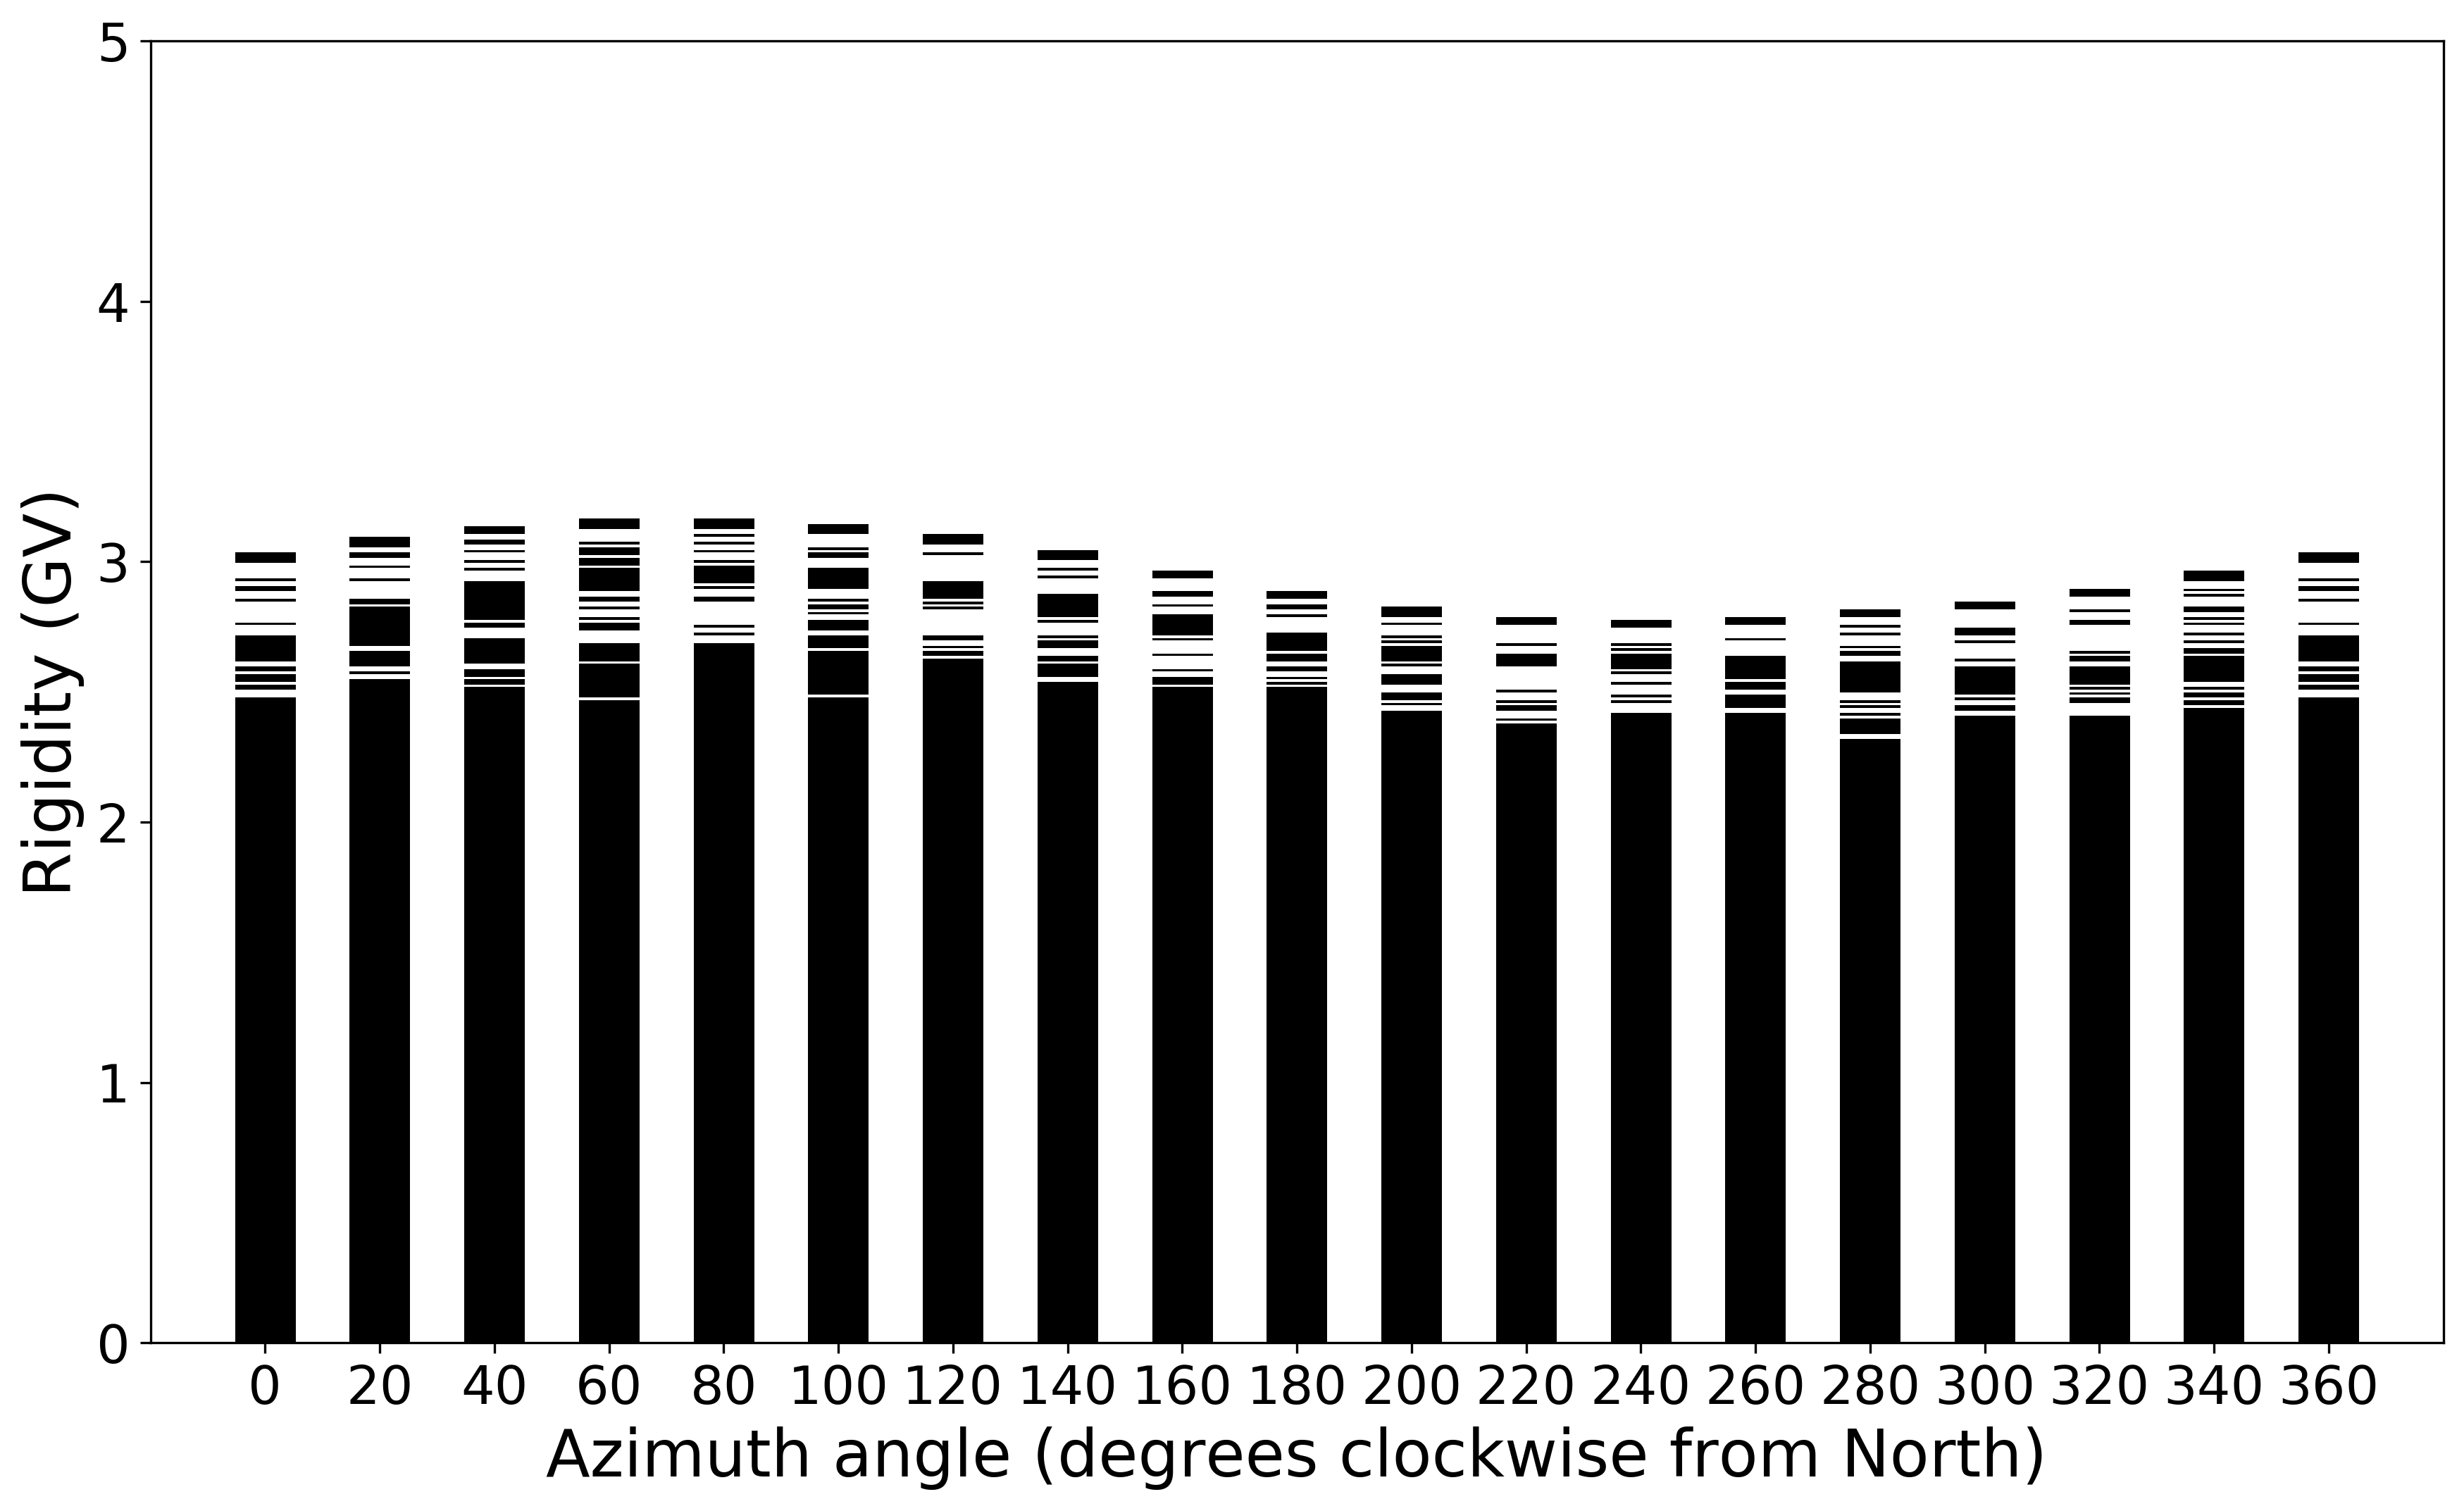
\includegraphics[width=0.46\columnwidth]{azm.png} }}
	
	\qquad
	
	\subfloat[ Zenith variation with fixed azimuth at  $0^\circ$ ]{
		{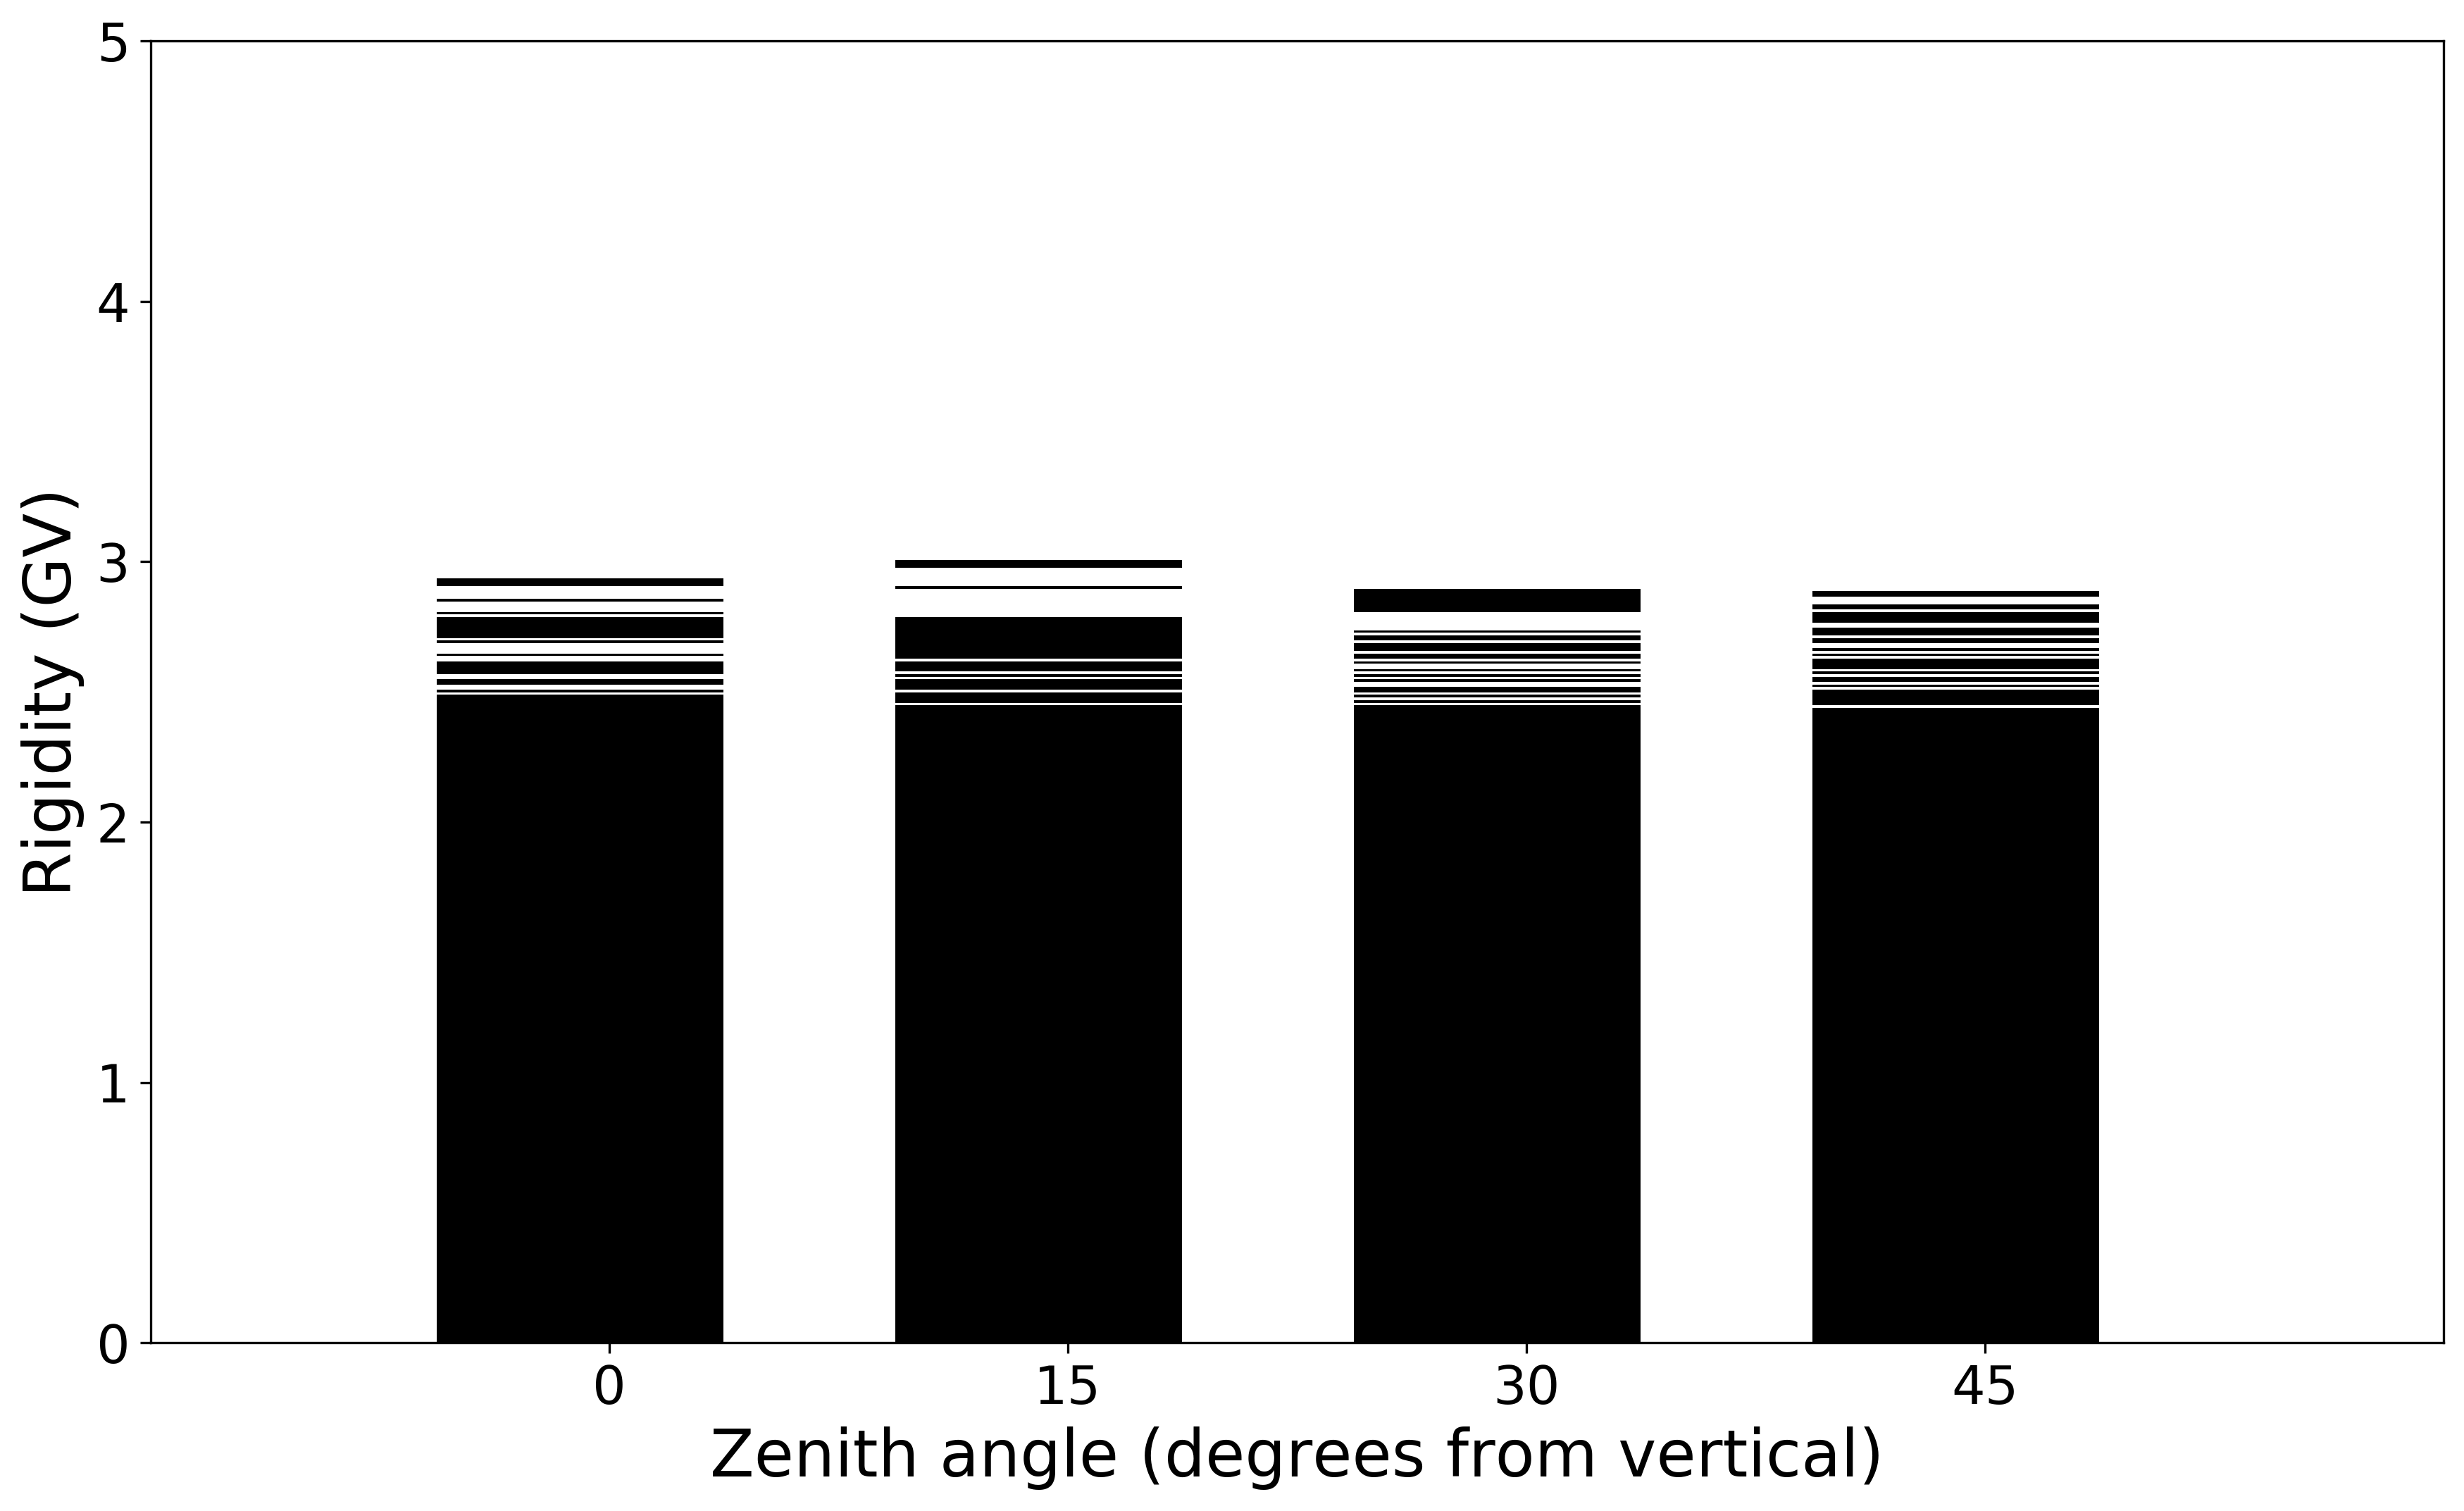
\includegraphics[width=0.46\columnwidth]{zen.png} }}
	
	\caption{ Azimuthal and zenth variations in the allowed and forbidden trajectories for HiSPARC station 501 on January 20th 2005 }
	\label{fig:R_C}
\end{figure}


From the results of the PLANETOCOSMICS simulations it was possible to calculate the rigidity cut-off for each HiSPARC station using equation~(\ref{eq:cut_off}). The cut-off rigidity calculated for the six HiSPARC stations for a vertical incidence upon the atmosphere (i.e. $0^\circ$ zenith angle) are shown in Table~\ref{tab:HS_stns} which show that there is little variation in $R_C$ between the HiSPARC stations and that they observe protons with rigidities in excess of $\sim 3$ GV. 


\begin{table}
	\begin{center}
		\caption{Properties of some of the HiSPARC stations: geographic longitude ($\lambda$), geographic latitude ($\phi$), altitude ($h$), and the geomagnetic vertical cut-off rigidity ($R_C$) calculated from the PLANETOCOSMICS simulations.}
		\label{tab:HS_stns}
		\begin{tabular}{l c c c c c}
			\hline
			& $R_C$  & $\lambda$ & $\phi$  & $h$  & No. Detectors\\
			Station Name/ID & [GV] & [deg] & [deg] & [m]  & \\
			\hline
			Nikhef/501 & 3.19 & 4.95 E & 52.36 N & 56.18 & 4 \\
			College Hageveld/203 & 3.18 & 4.63 E  & 52.35 N & 53.71  & 2 \\
			Leiden/3001 & 3.23 & 4.45 E & 52.17 N & 54.08 & 2 \\
			Eindhoven/8001  & 3.44 & 5.49 E & 51.45 N & 70.12 & 2 \\
			Birmingham University/14001  & 3.06 & 1.93 W & 52.45 N & 204.14 & 4  \\
			%20003 & 2.30 & 10.20 E & 56.17 N & 84.38 & 2 \\
			\hline
		\end{tabular}
	\end{center}
\end{table}

The small variation between HiSPARC stations is due to their close proximity in geographic latitude and longitude. The values of $R_C$ calculated for the HiSPARC stations suggest that they should be able to observe higher energy SCRs, but may not be as susceptible as the higher latitude NMs where the effects of GLEs are highly observable.



 

%%%%%%%%%%%%%%%%%%%%%%%%%%%%%%%%%%%%%%%%%%%%%%%%%%%%%%%%%%%%%%%%%%%%%
%%%%%%%%%%%%%%%%%%%%%%%%%%%%%%%%%%%%%%%%%%%%%%%%%%%%%%%%%%%%%%%%%%%%%
\section{HiSPARC Observations}\label{sec:HS_obs}


[discuss preliminary observation of space weather FDs and GLEs for the events and singles data...]

[end with discussion on unknown PCRs observable and the effect of atmospheric weather conditions that need to be accounted for]

The effects of space weather on CRs has been outlined in [REF intro]. It was highlighted during communication with the UK Met Office that observations of GLEs are of more interest and importance to space weather forecasts and nowcasts. FDs are of lower interest and importance, however they were still searched for within the HiSPARC data. The events that were looked for within the HiSPARC data are outlined in Table~\ref{tab:space_weather_events}.

\begin{table}
	\begin{center}
		\caption{Space weather events investigated within the HiSPARC data. The percentage change column provides a reference of how much the CR counts observed by the NM station at Oulu (R$_c$=0.81~GV) increased of decreased by, due to the space weather event.}
		\label{tab:space_weather_events}
		\begin{tabular}{c c c | c c}
		\hline
		{\bf GLE Onset} & {\bf GLE} & {\bf \% Change (Oulu)} & {\bf FD Onset} & {\bf \% Change (Oulu)}\\
		\hline
		{13/12/2006} & {70} & {$\sim 100\%$} & {08/03/2012} & {$\sim 5\%$}  \\
		{17/05/2012} & {71} & {$\sim 15\%$} & {14/07/2012} & {$\sim 3\%$} \\
		{10/09/2017} & {72} & {$\sim 5\%$} & {21/12/2014} & {$\sim 5\%$} \\
		{} & {} & {} & {06/09/2017} & {$\sim 2\%$} \\
		{} & {} & {} & {07/09/2017} & {$\sim 8\%$} \\
		\hline
		\end{tabular}
	\end{center}
\end{table}



%%%%%%%%%%%%%%%%%%%%%%%%%%%%%%%%%%%%%%%%%%%%%%%%%%%%%%%%%%%%%%%%%%%%%
\subsection{HiSPARC Observations of Ground Level Enhancements}

Initial searches for evidence of GLEs within the HiSPARC data were conducted for GLE 70, 71, and 72, as they arethe only GLEs that span the operational epoch of the HiSPARC network.

Figure~\ref{fig:GLE_70}...

\begin{figure}[h]
	\centering
	\subfloat[HS 501 (Nikhef)]{
		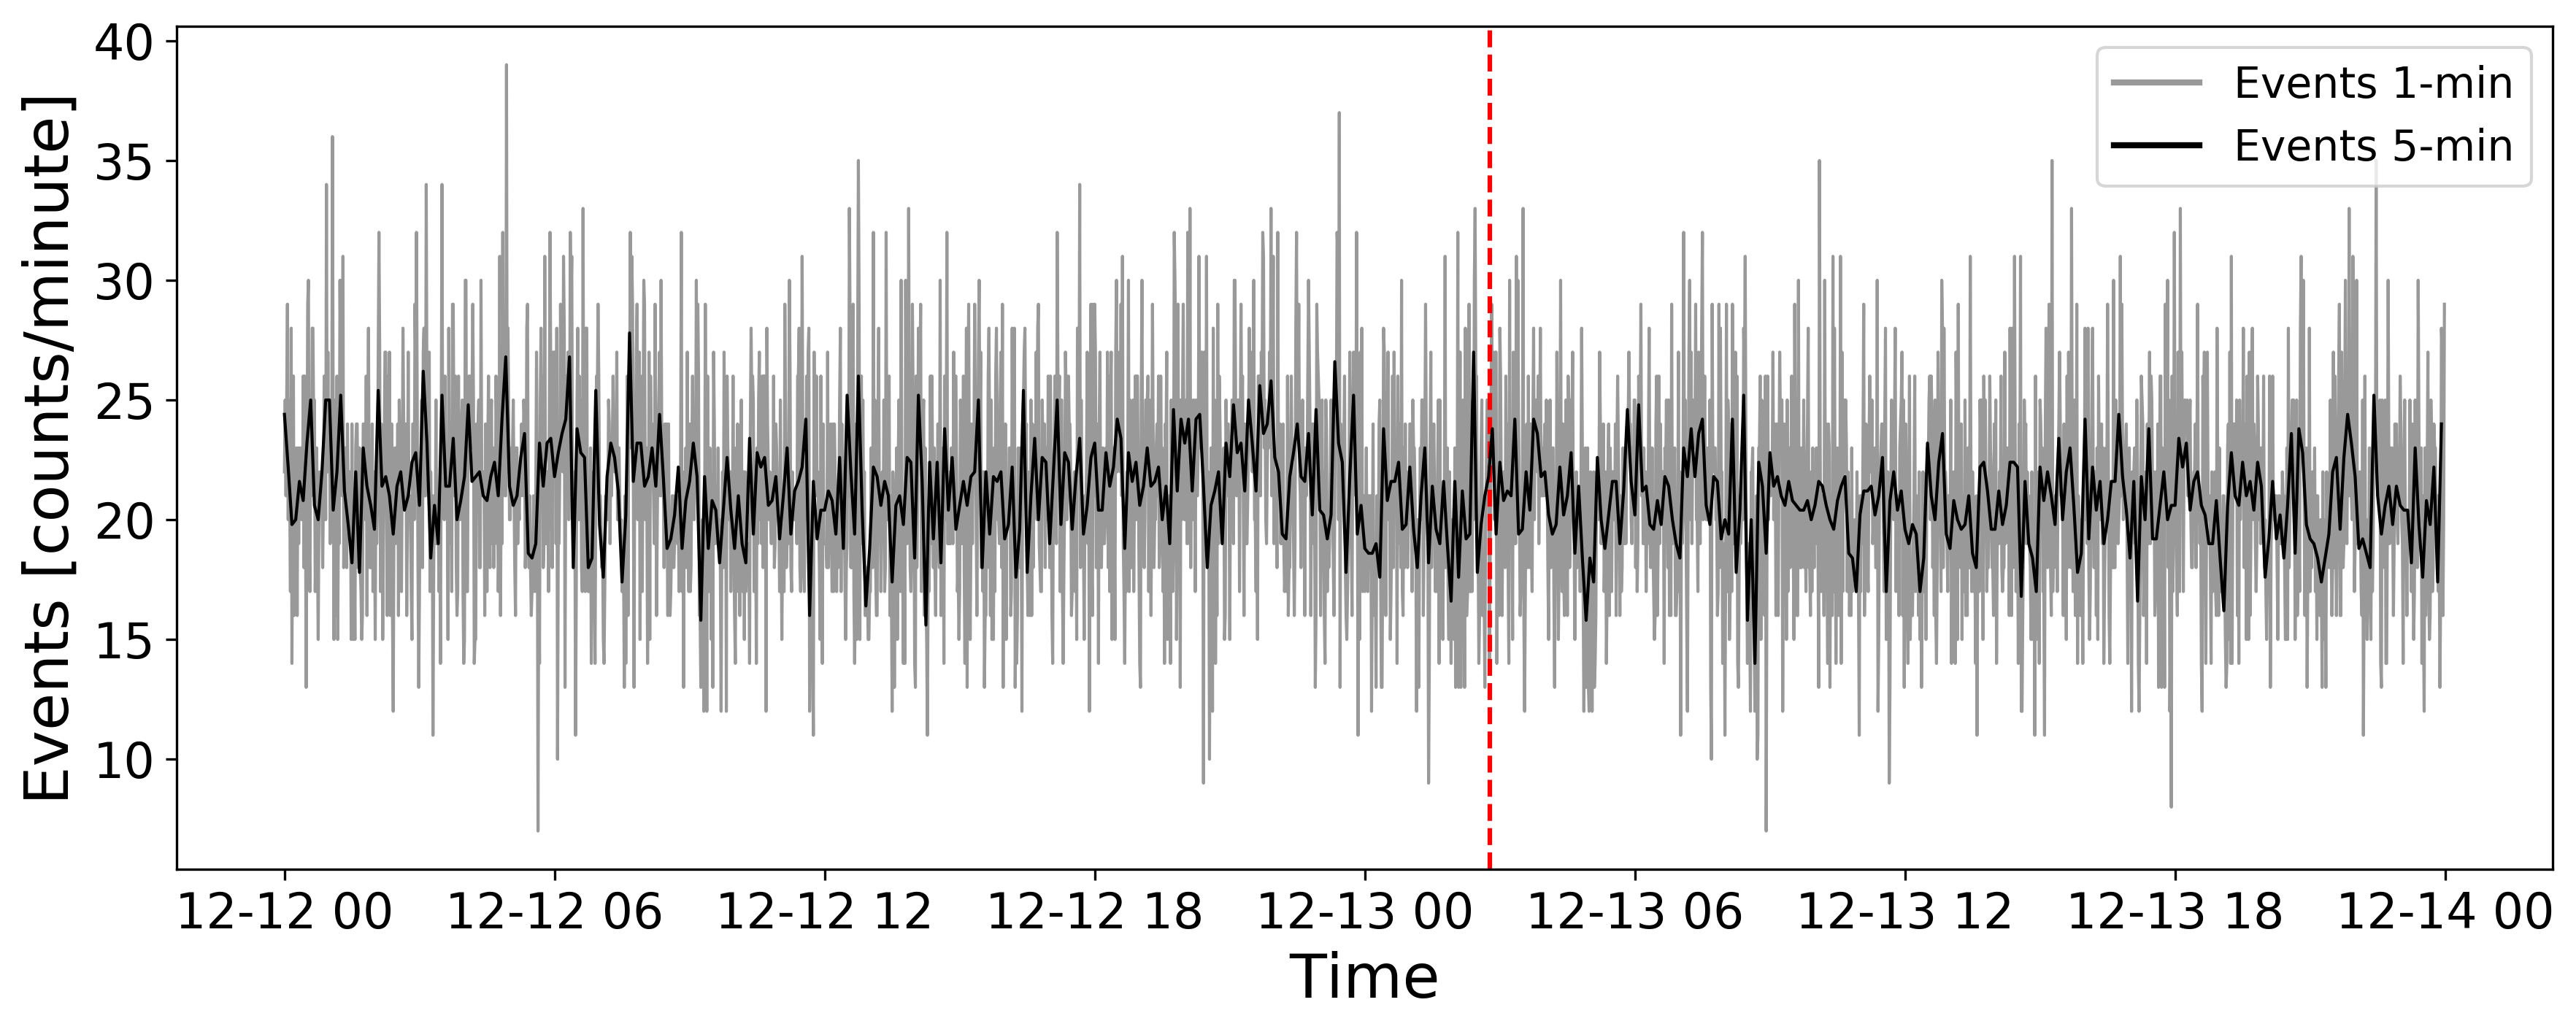
\includegraphics[width=0.48\columnwidth]{GLE70_501.png}
		\label{fig:GLE70_501}}
	%\qquad
	\subfloat[HS 3001 (Universiteit Leiden)]{
		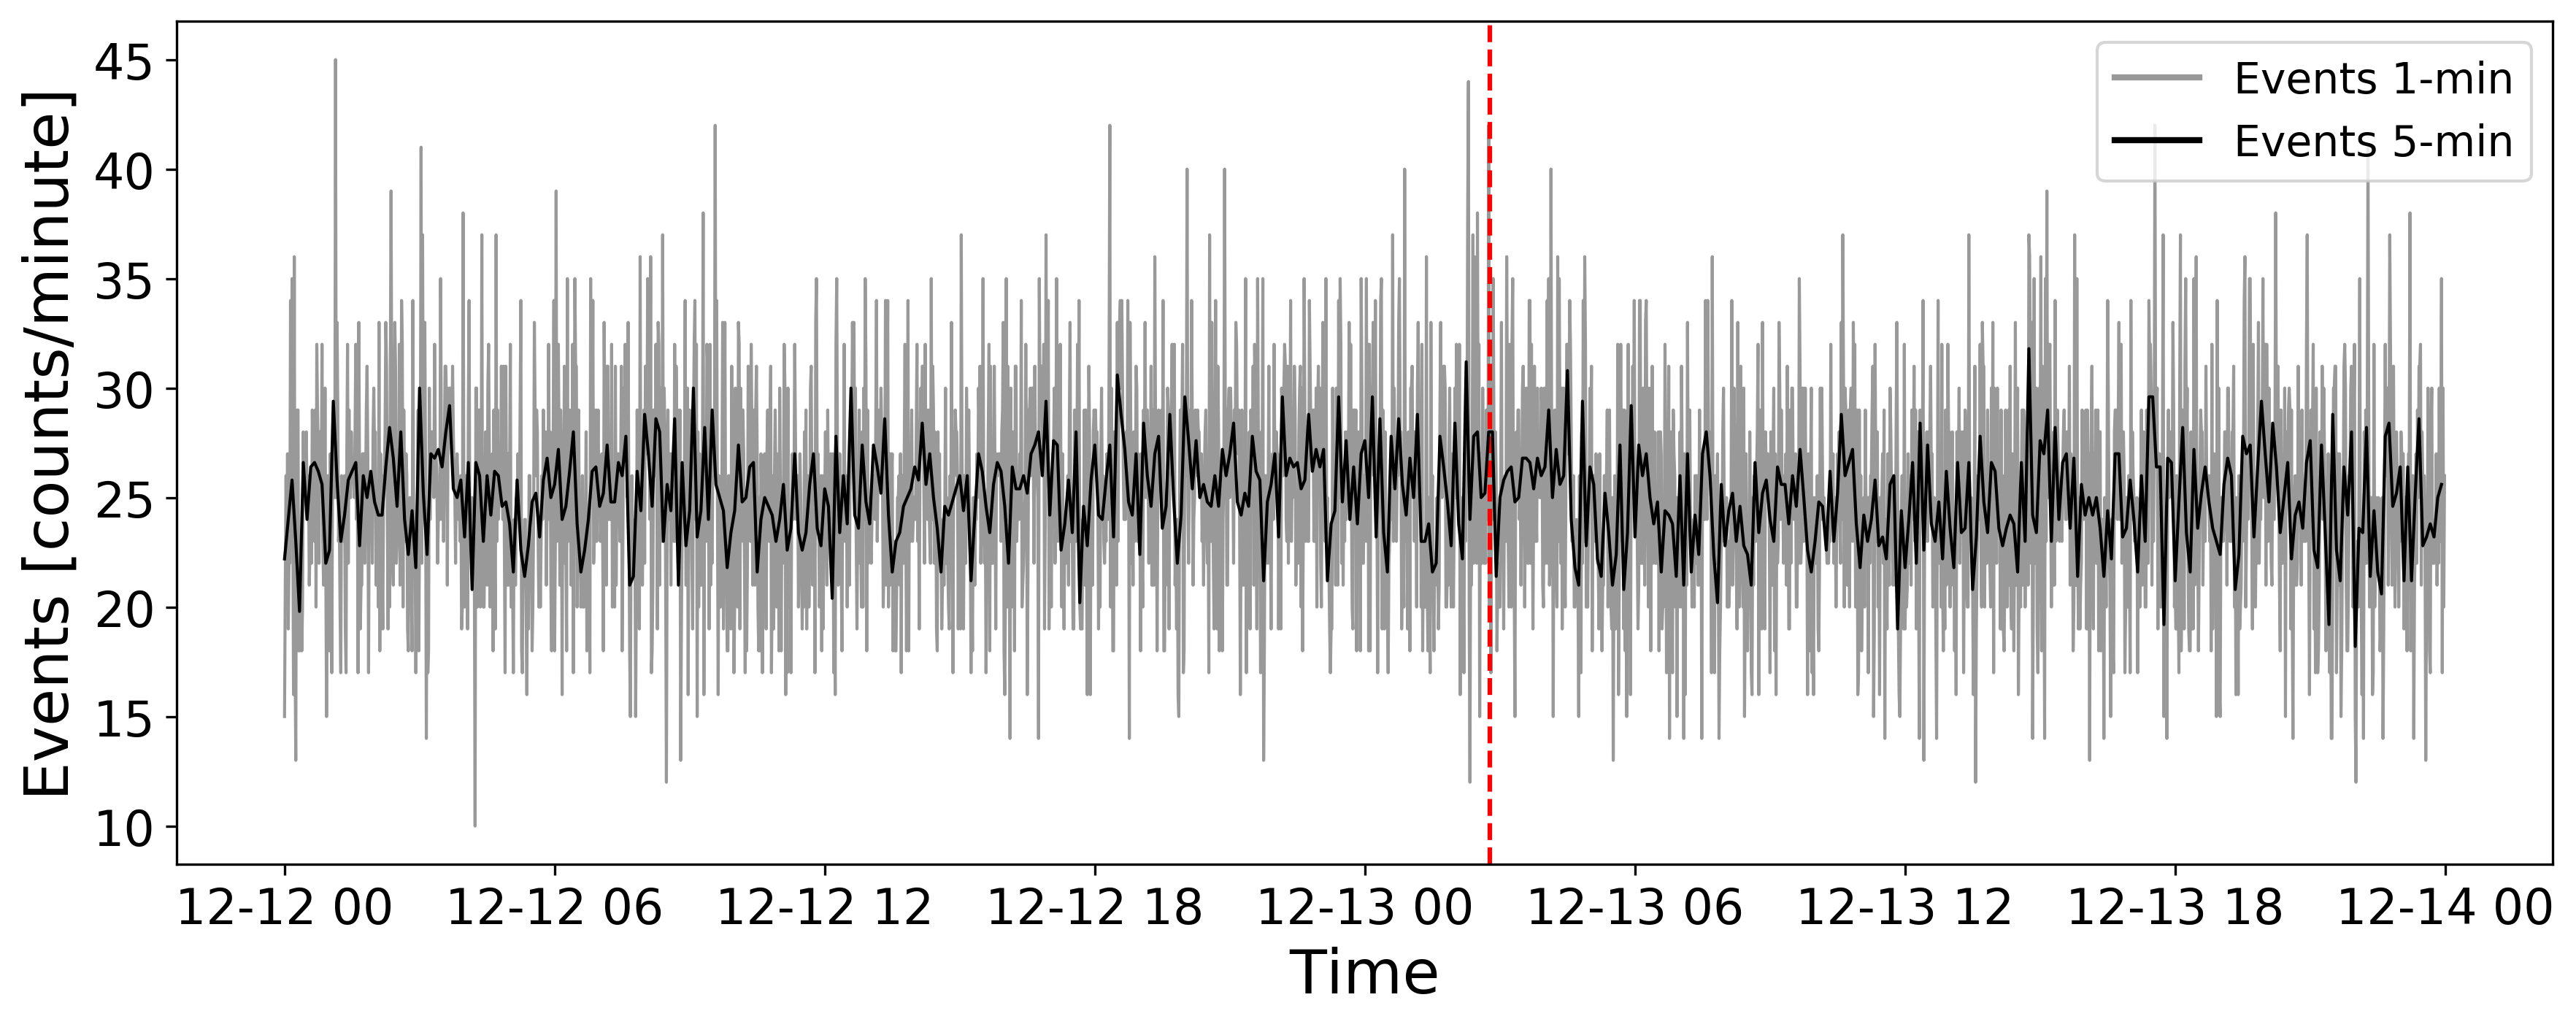
\includegraphics[width=0.48\columnwidth]{GLE70_3001.png}
		\label{fig:GLE70_3001}}
	
	\caption{HiSPARC data for stations 501 and 3001 around the epoch of GLE 70. The plot shows the minute-averaged and 5-minute-averaged trigger events between detectors within the station. The vertical red, dashed line depicts the approximate onset time of the GLE.}
	\label{fig:GLE_70}
\end{figure}


Figure~\ref{fig:GLE_71}...

\begin{figure}[h]
	\centering
	\subfloat[HS 8001 (Eindhoven)]{
		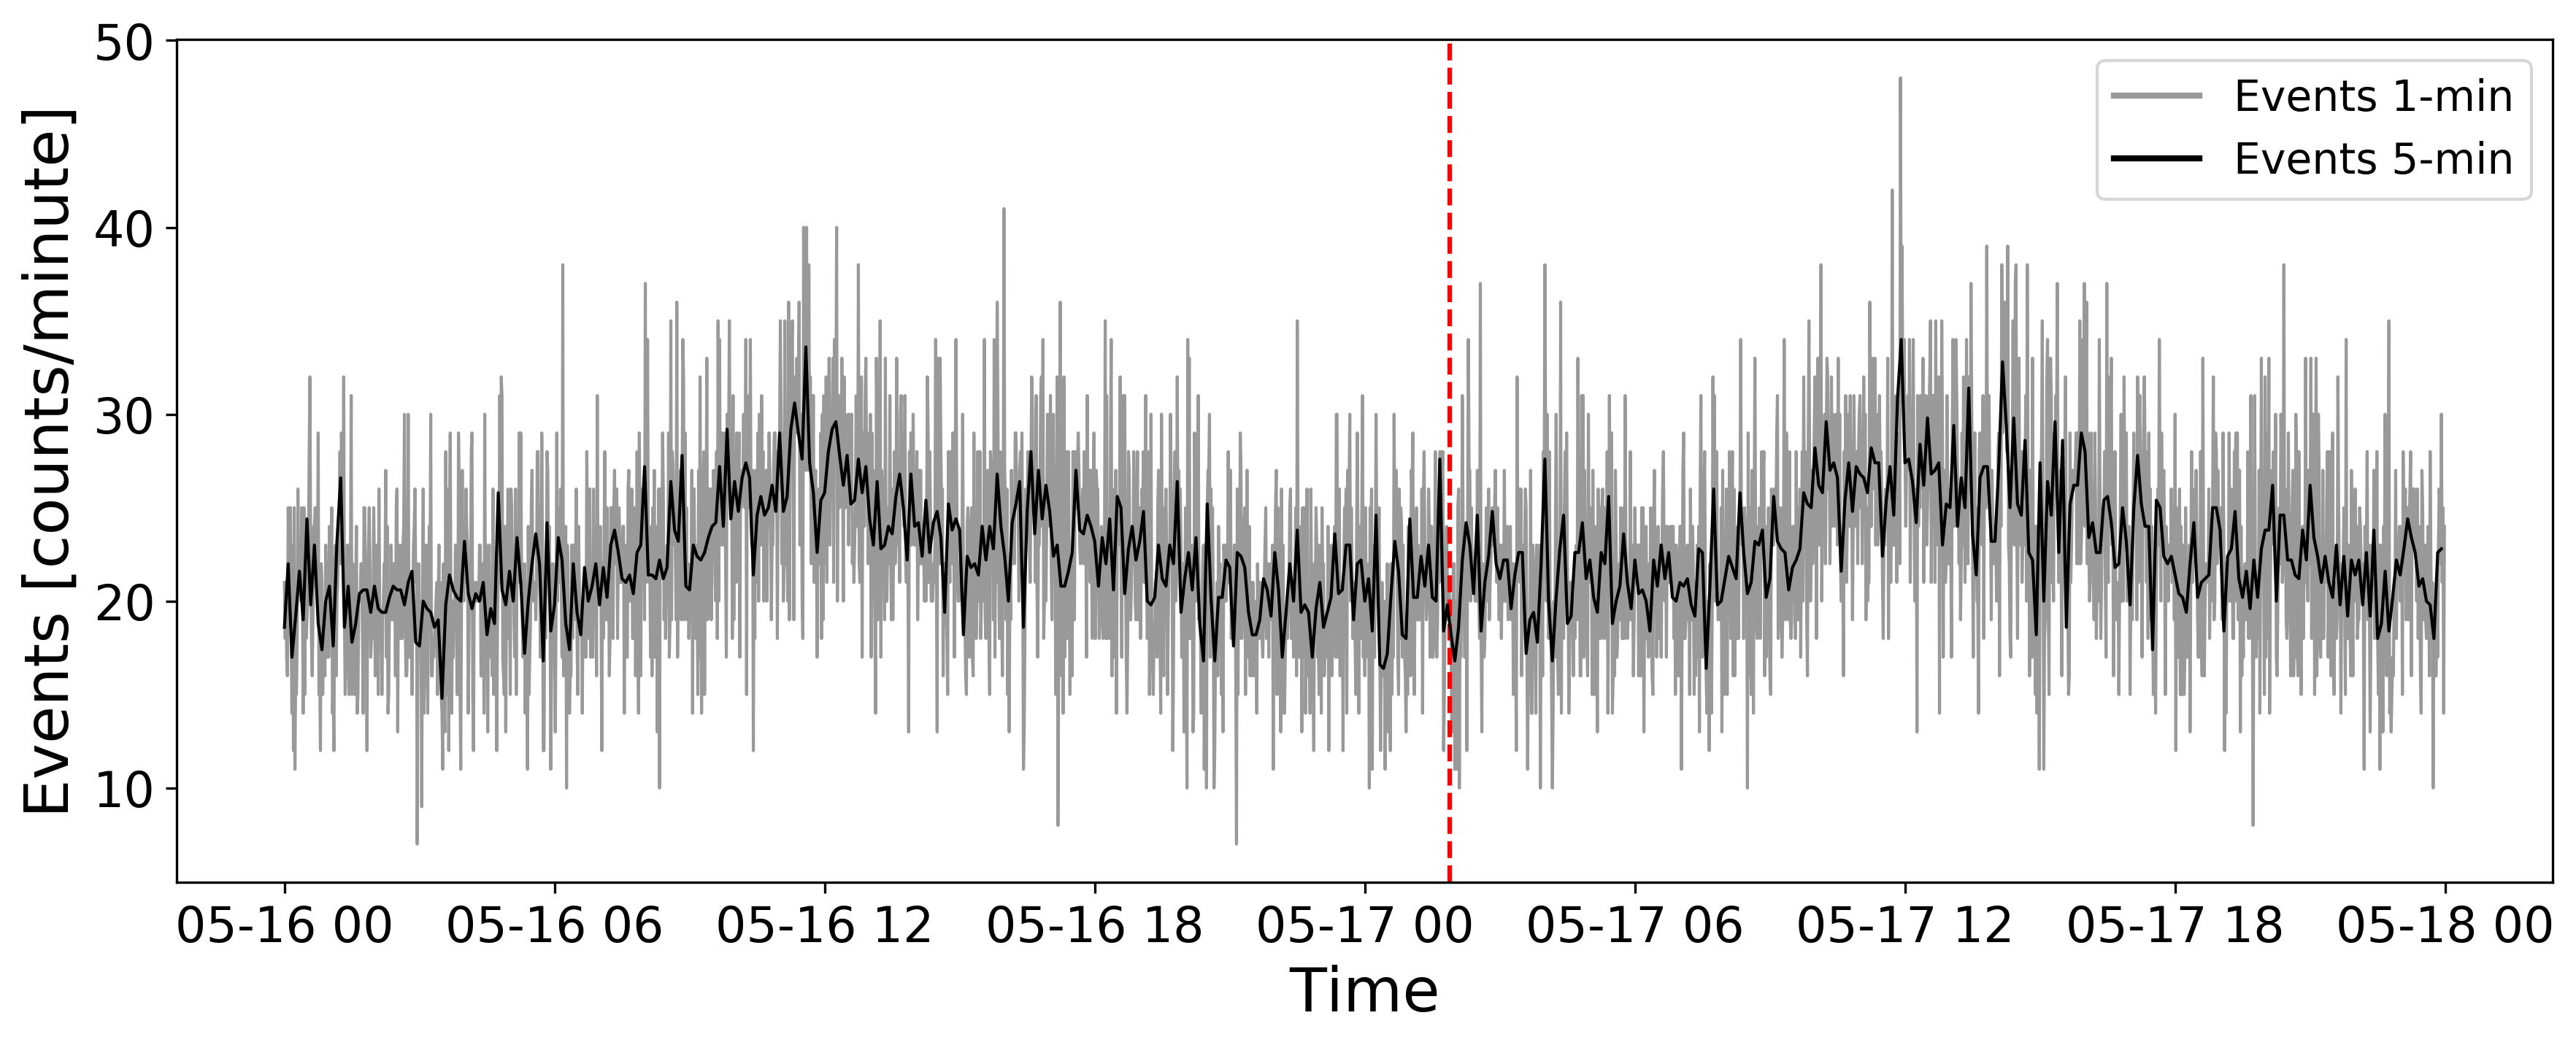
\includegraphics[width=0.48\columnwidth]{GLE71_8001.png}
		\label{fig:GLE71_8001}}
	%\qquad
	\subfloat[HS 3001 (Universiteit Leiden)]{
		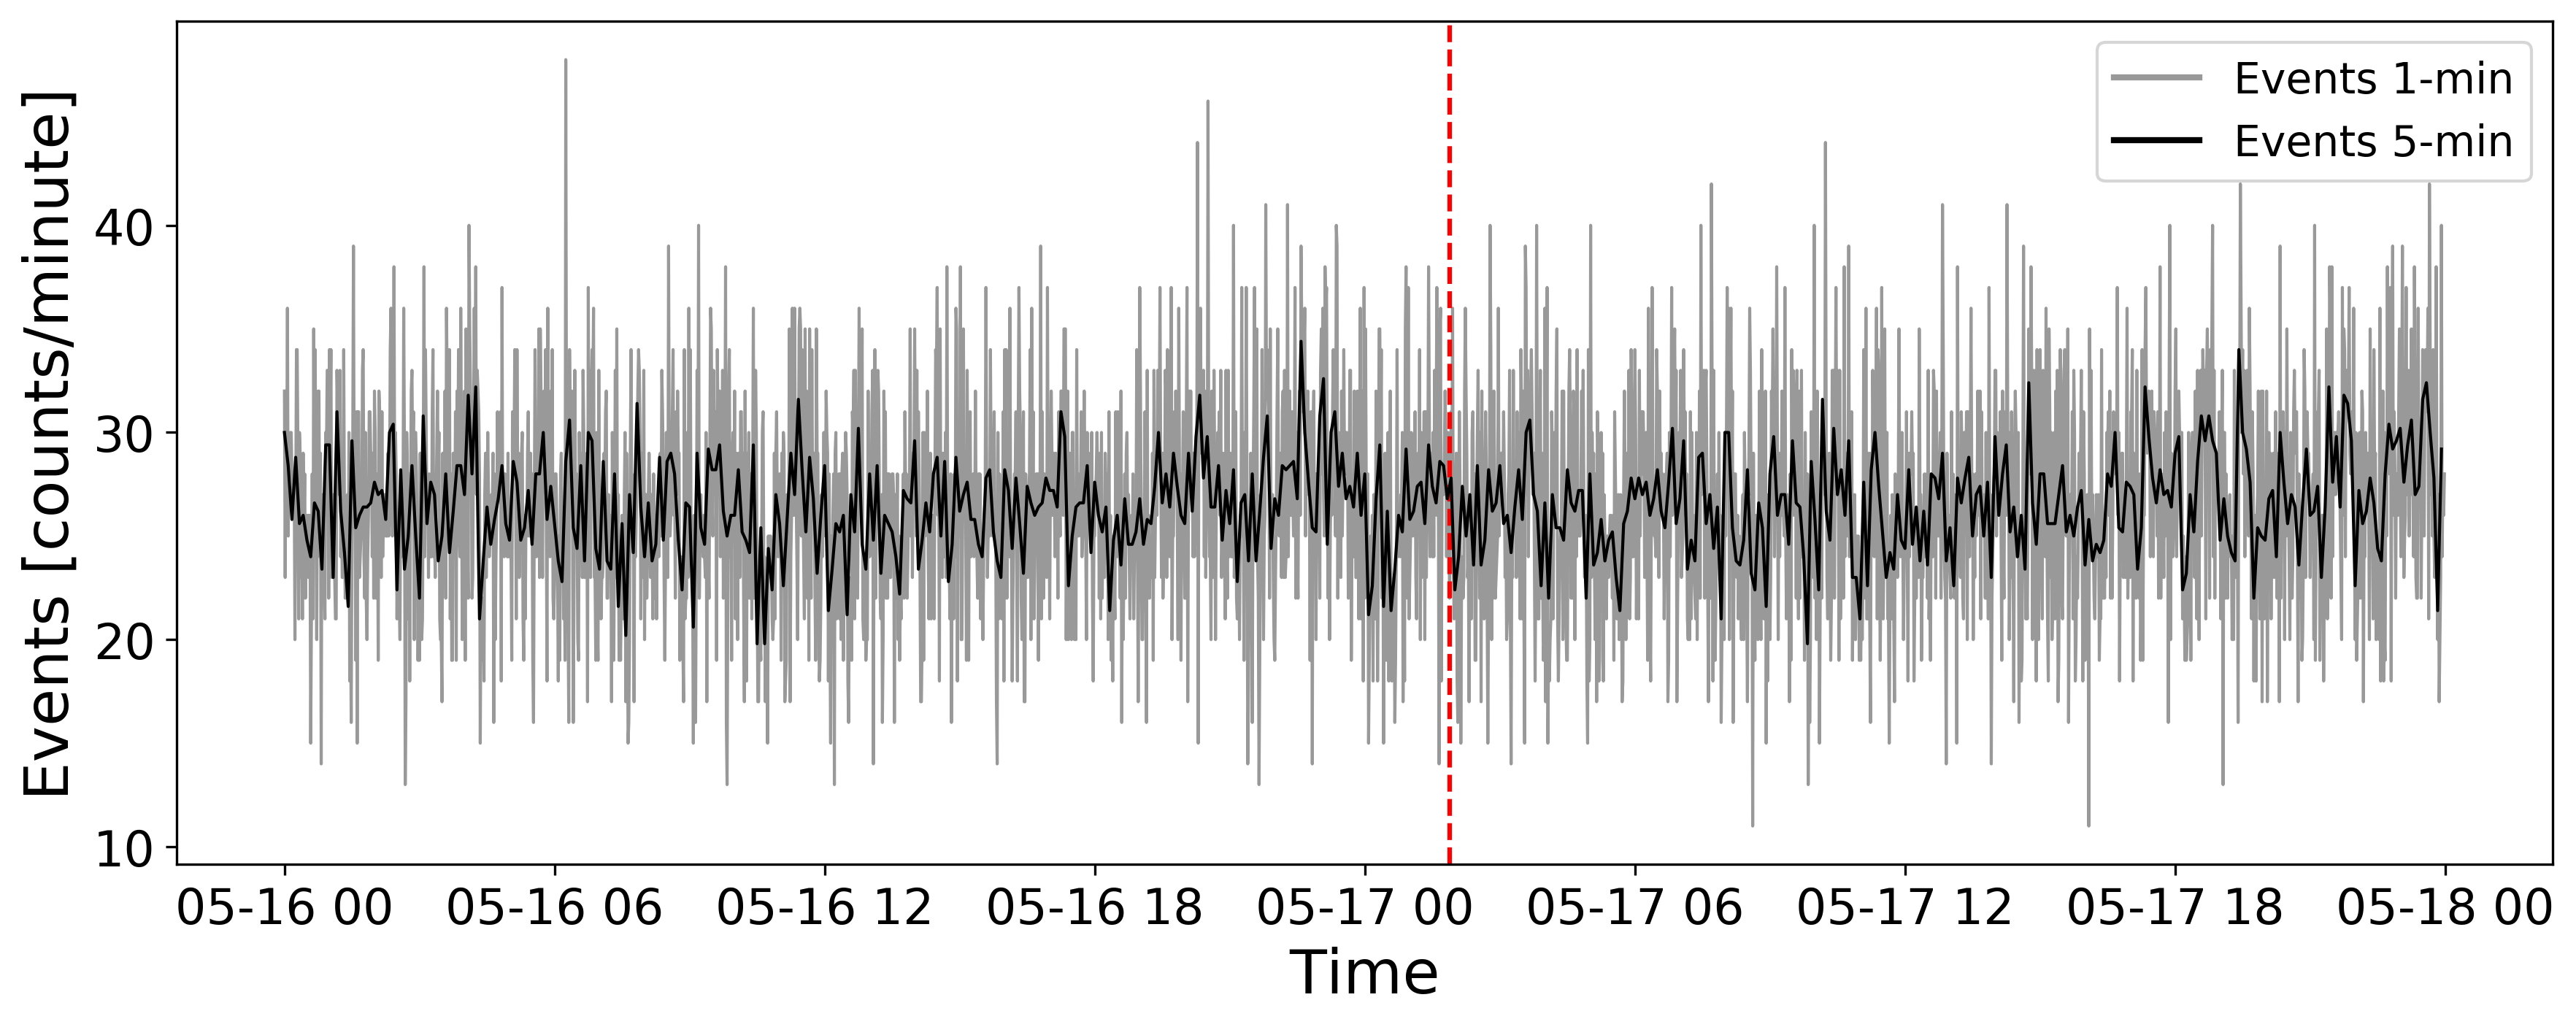
\includegraphics[width=0.48\columnwidth]{GLE71_3001.png}
		\label{fig:GLE71_3001}}
	
	\caption{HiSPARC data for stations 8001 and 3001 around the epoch of GLE 71. The plot shows the minute-averaged and 5-minute-averaged trigger events between detectors within the station. The vertical red, dashed line depicts the approximate onset time of the GLE.}
	\label{fig:GLE_71}
\end{figure}


Figure~\ref{fig:GLE_72}...

\begin{figure}[ht]
	\centering
	\subfloat[HS 501 (Nikhef)]{
		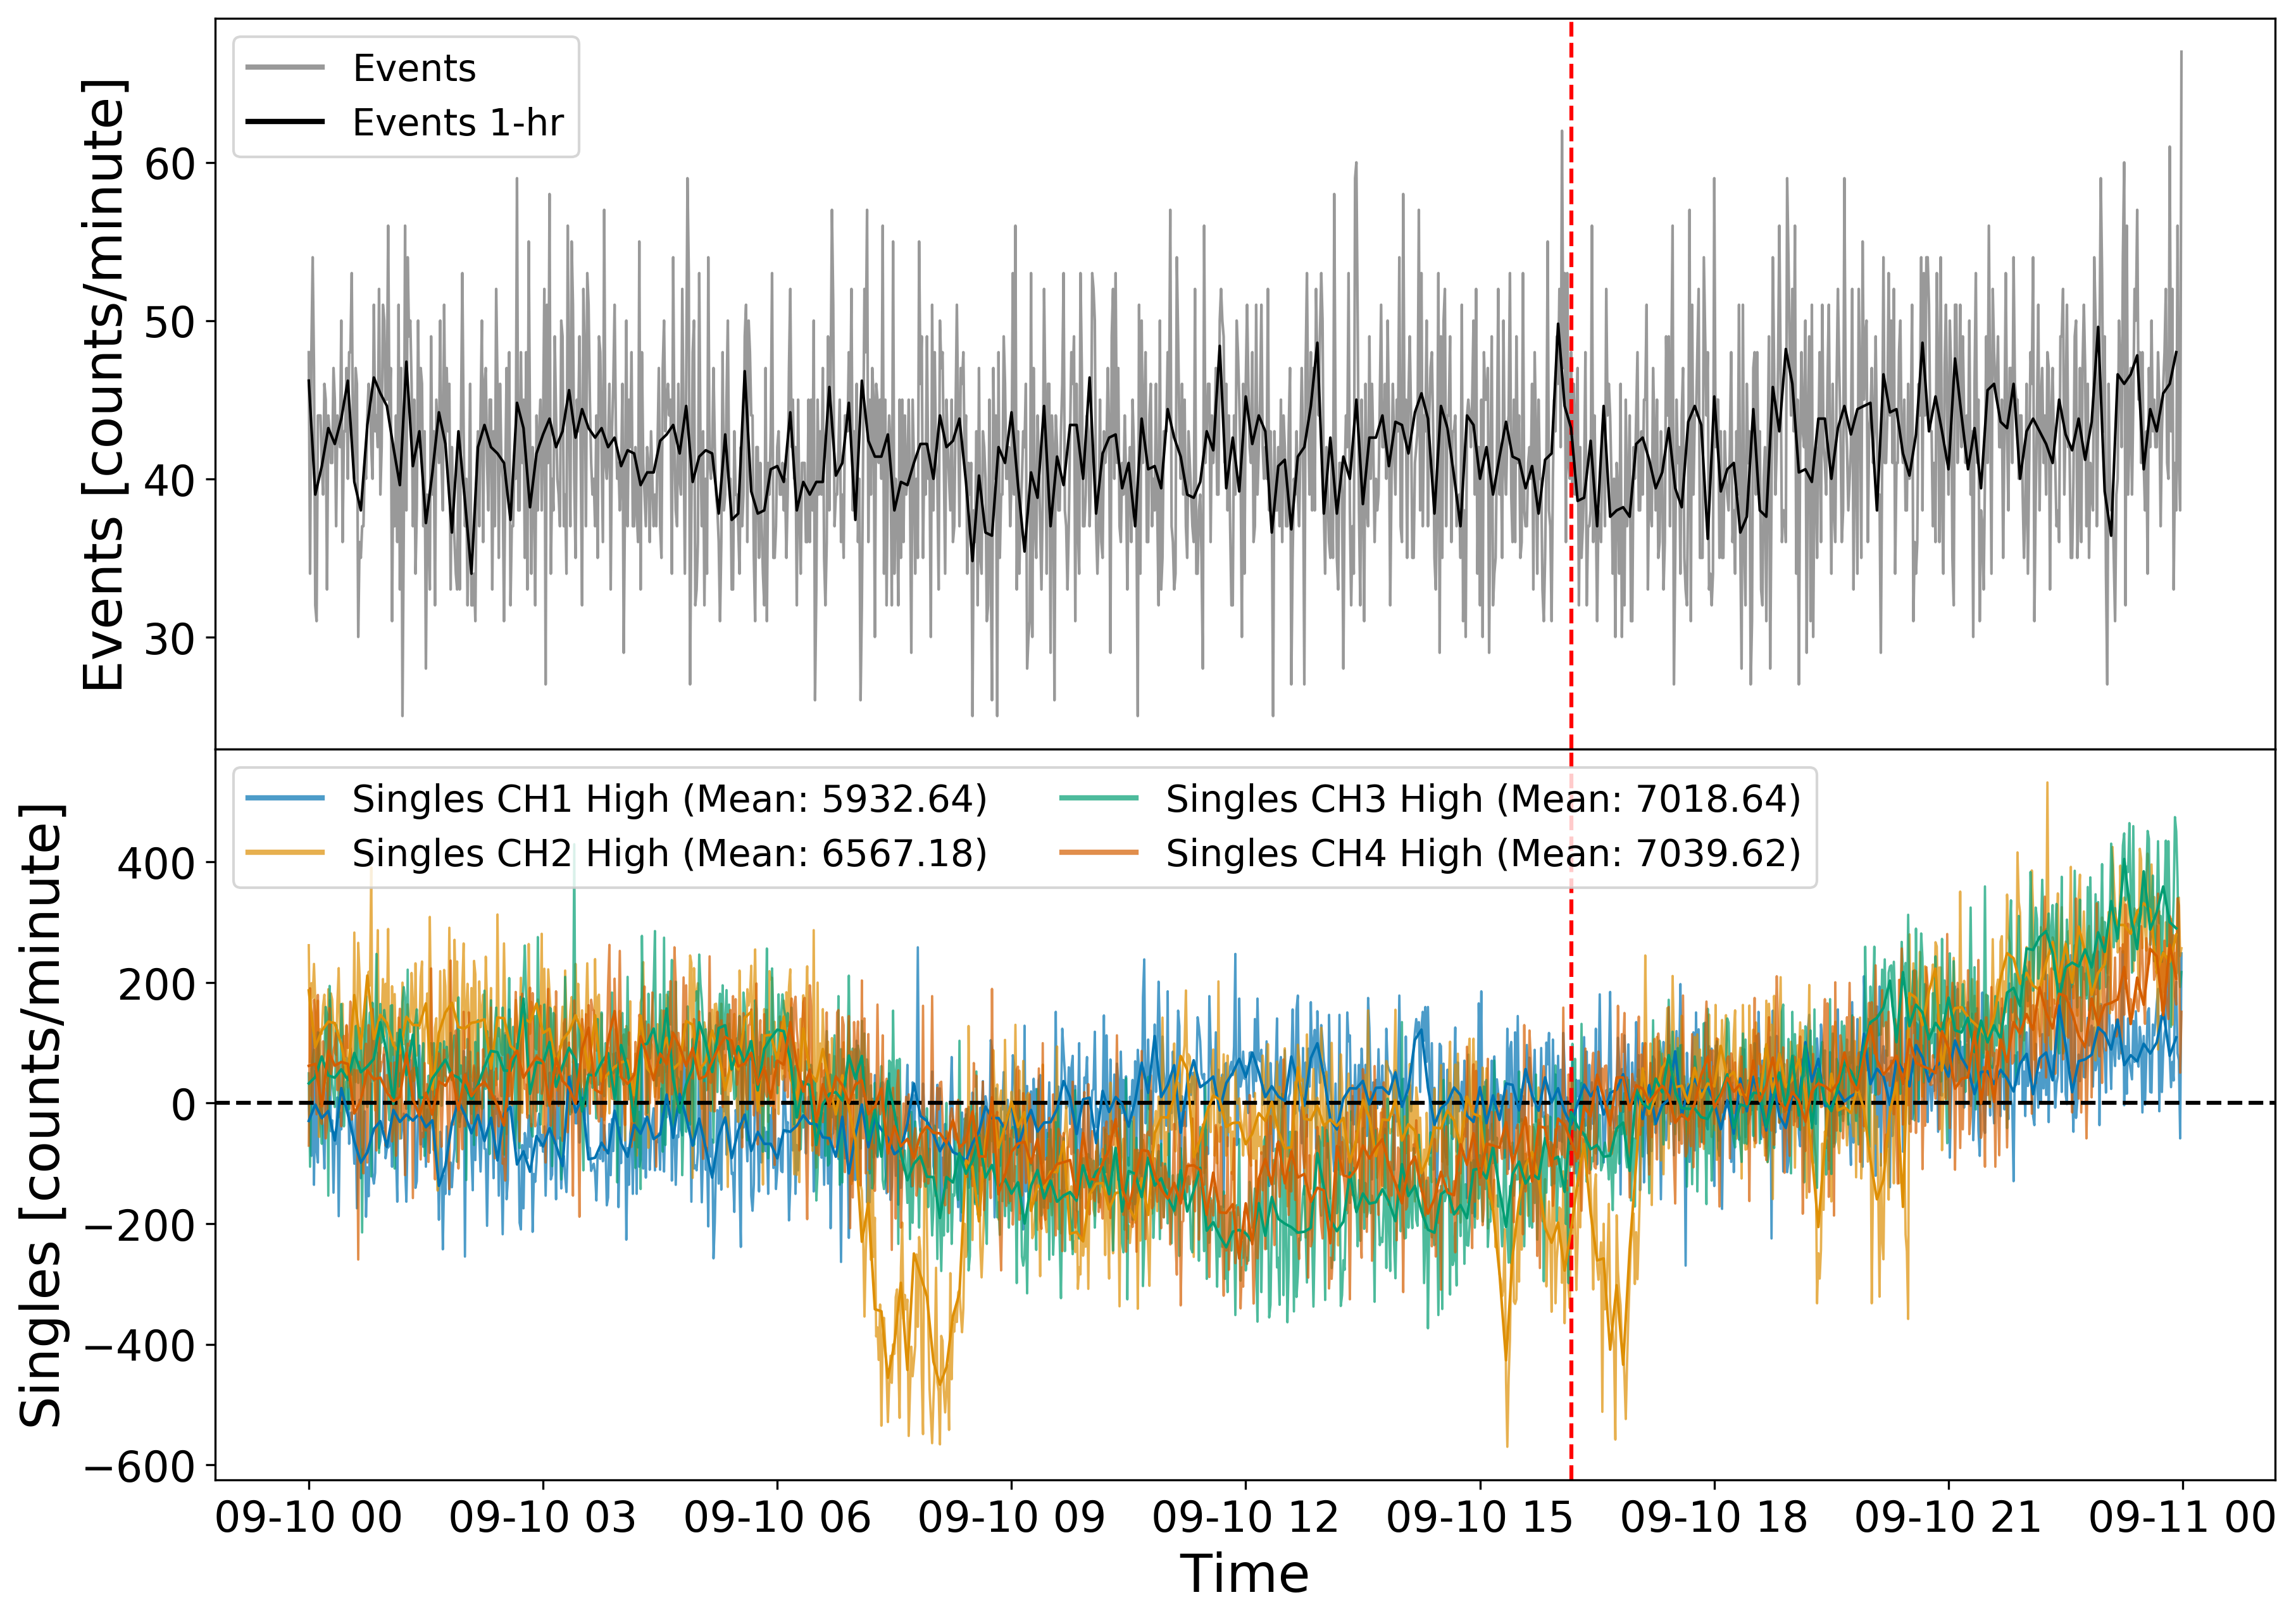
\includegraphics[width=0.48\columnwidth]{GLE72_501.png}
		\label{fig:GLE72_501}}
	%\qquad
	\subfloat[HS 203 (College Hageveld)]{
		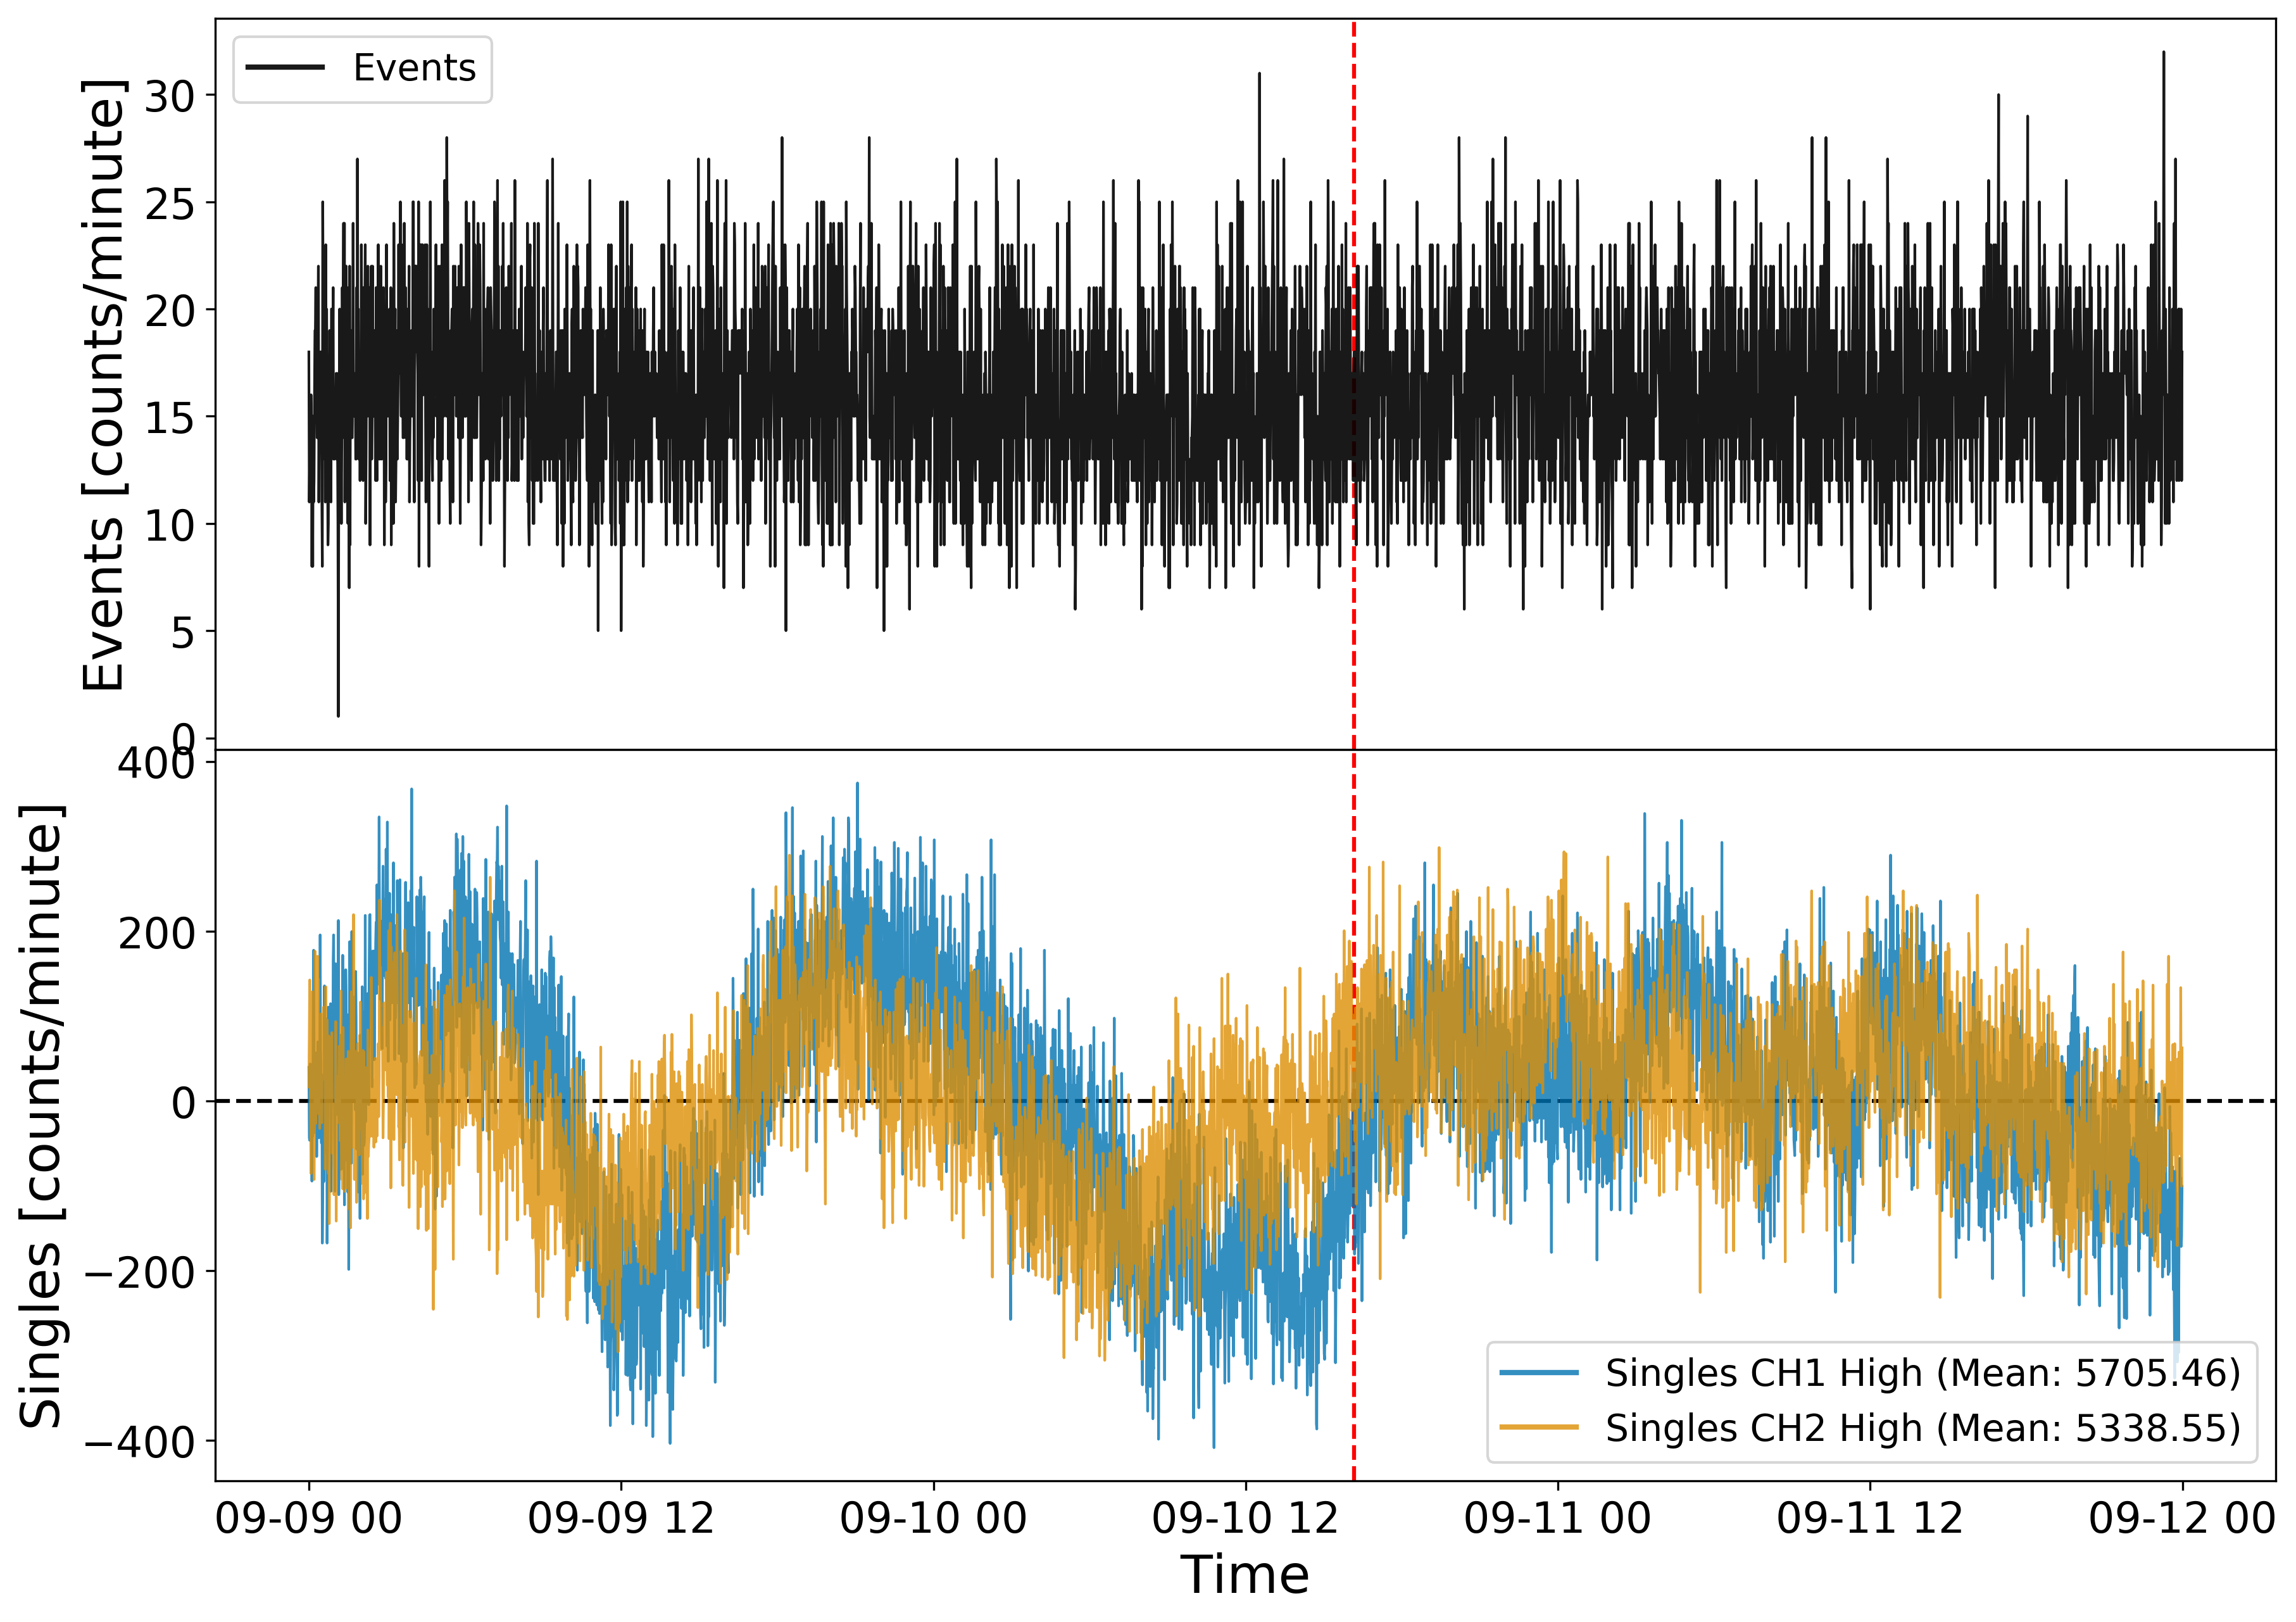
\includegraphics[width=0.48\columnwidth]{GLE72_203.png}
		\label{fig:GLE72_203}} \\
	
	\qquad
	
	\subfloat[HS 8001 (Eindhoven)]{
		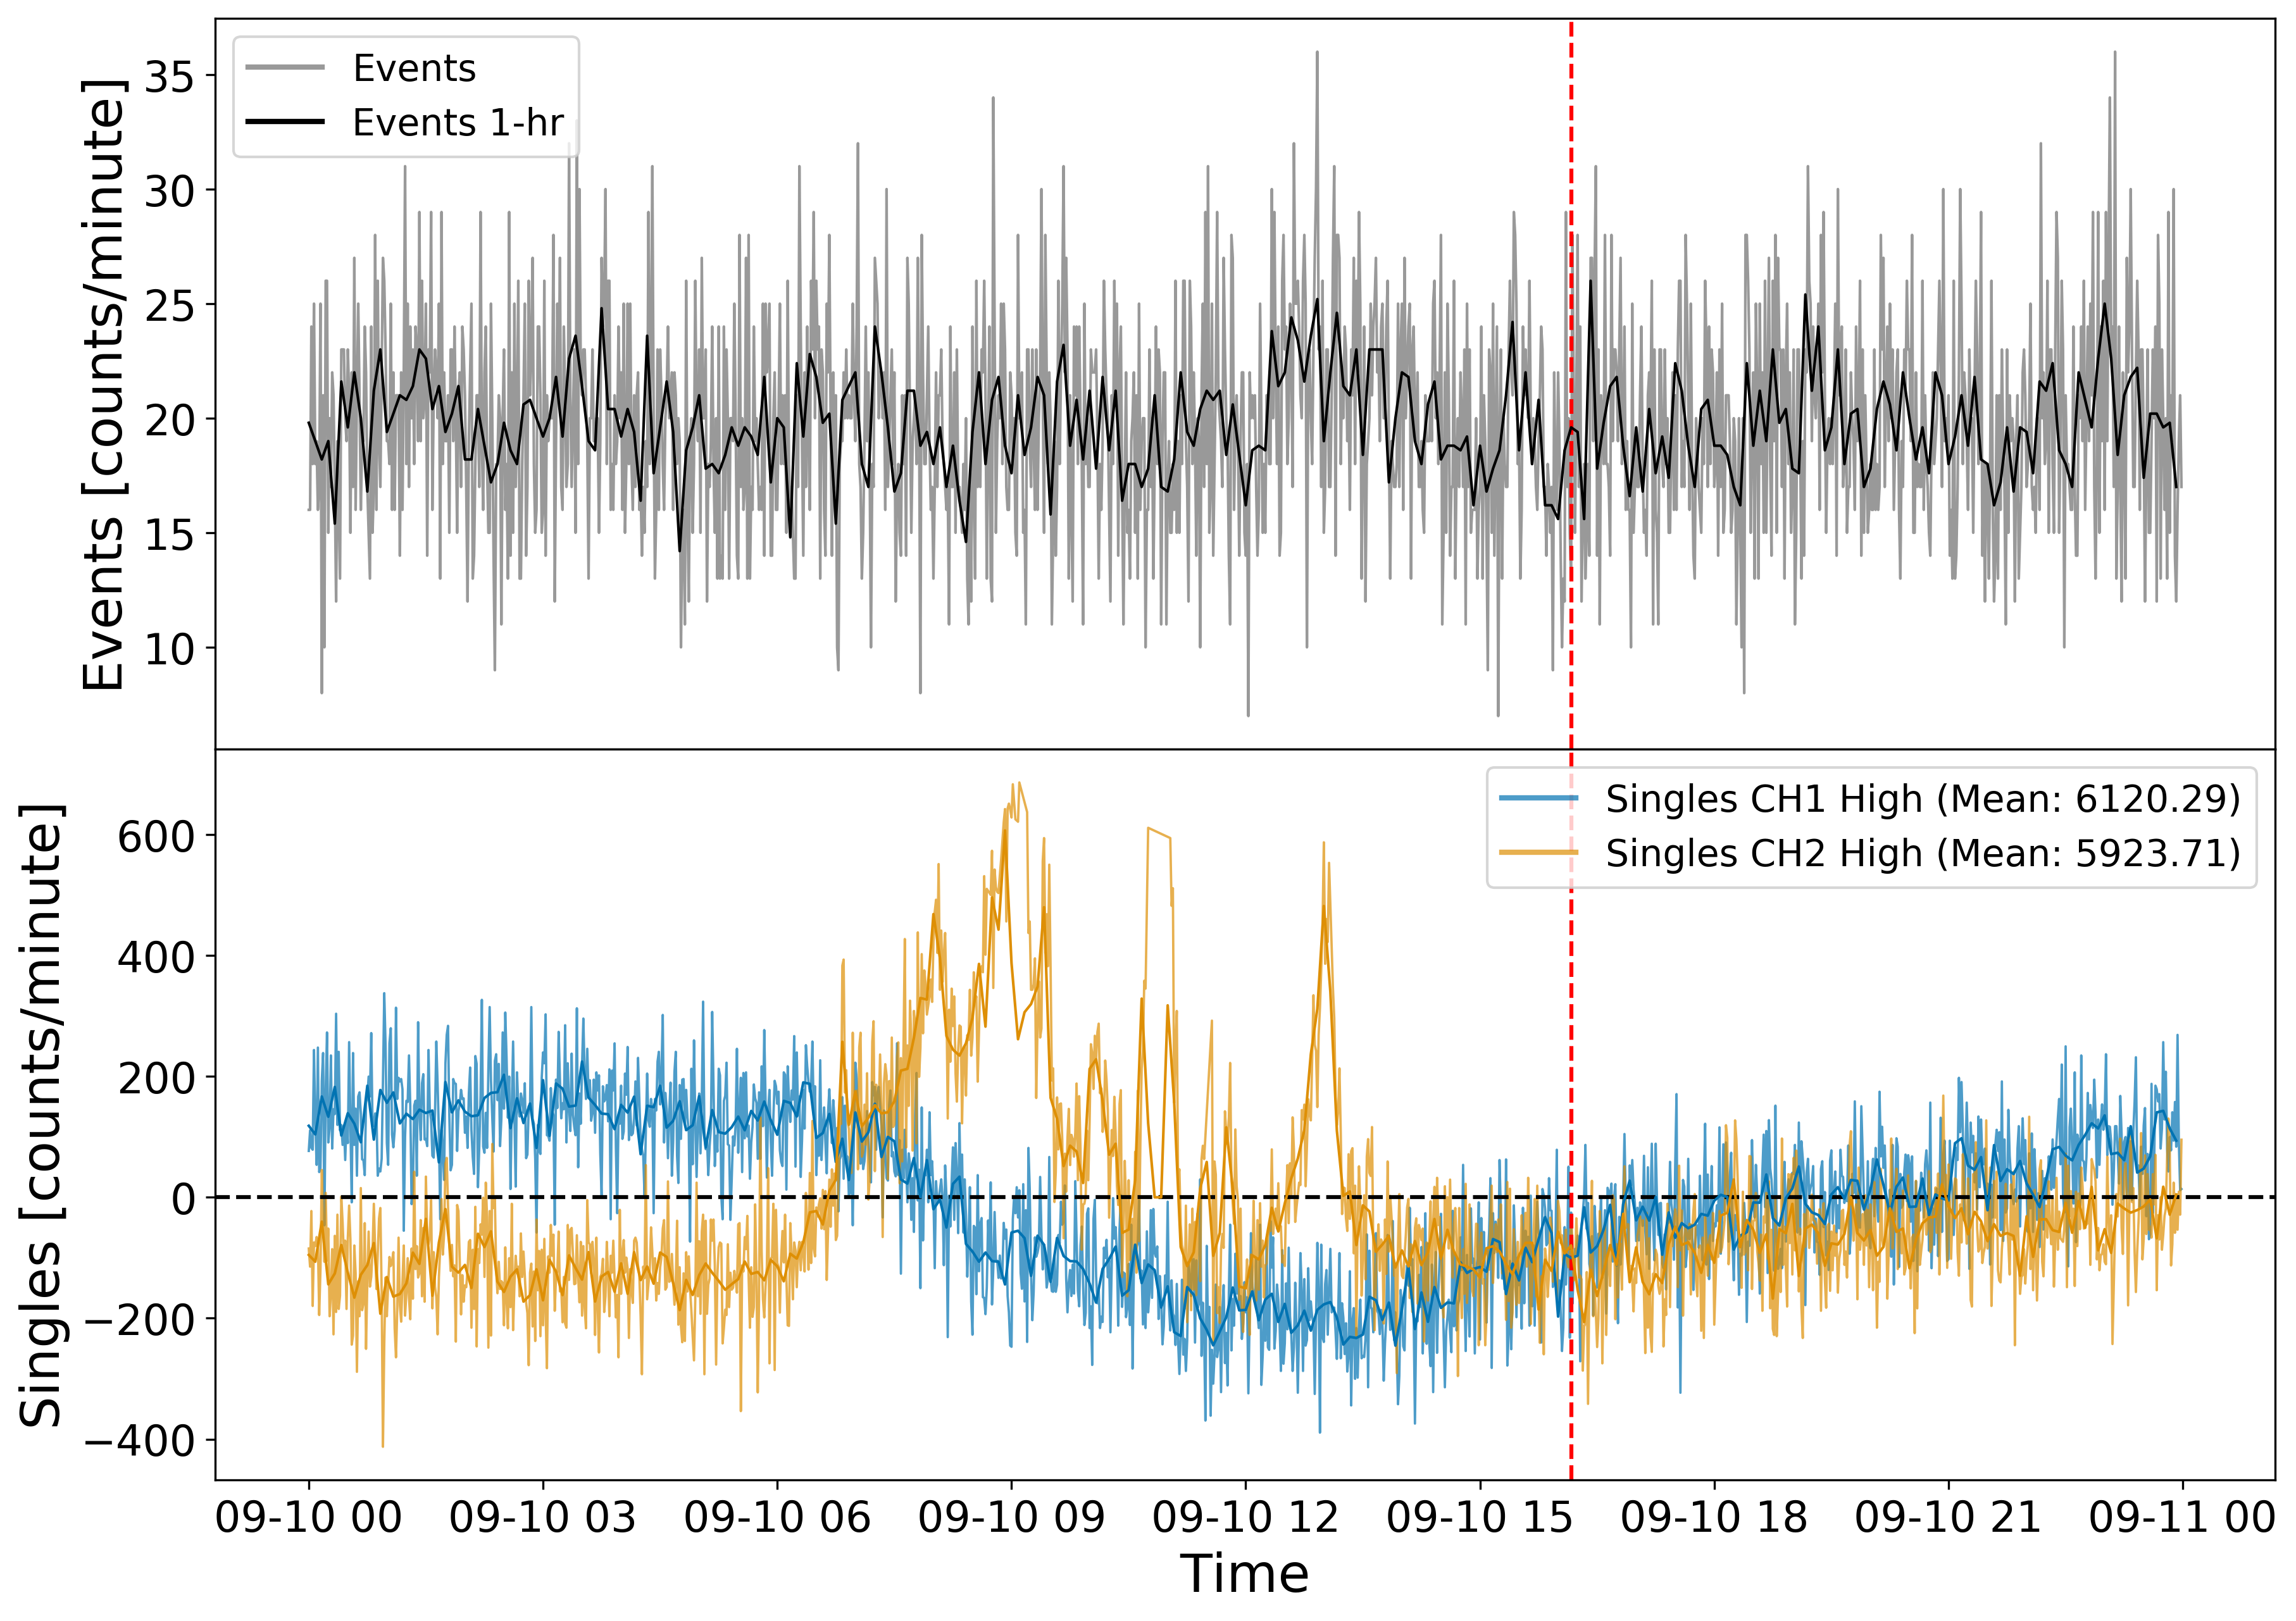
\includegraphics[width=0.48\columnwidth]{GLE72_8001.png}
		\label{fig:GLE72_8001}}
	%\qquad
	\subfloat[HS 14001 (Birmingham University)]{
		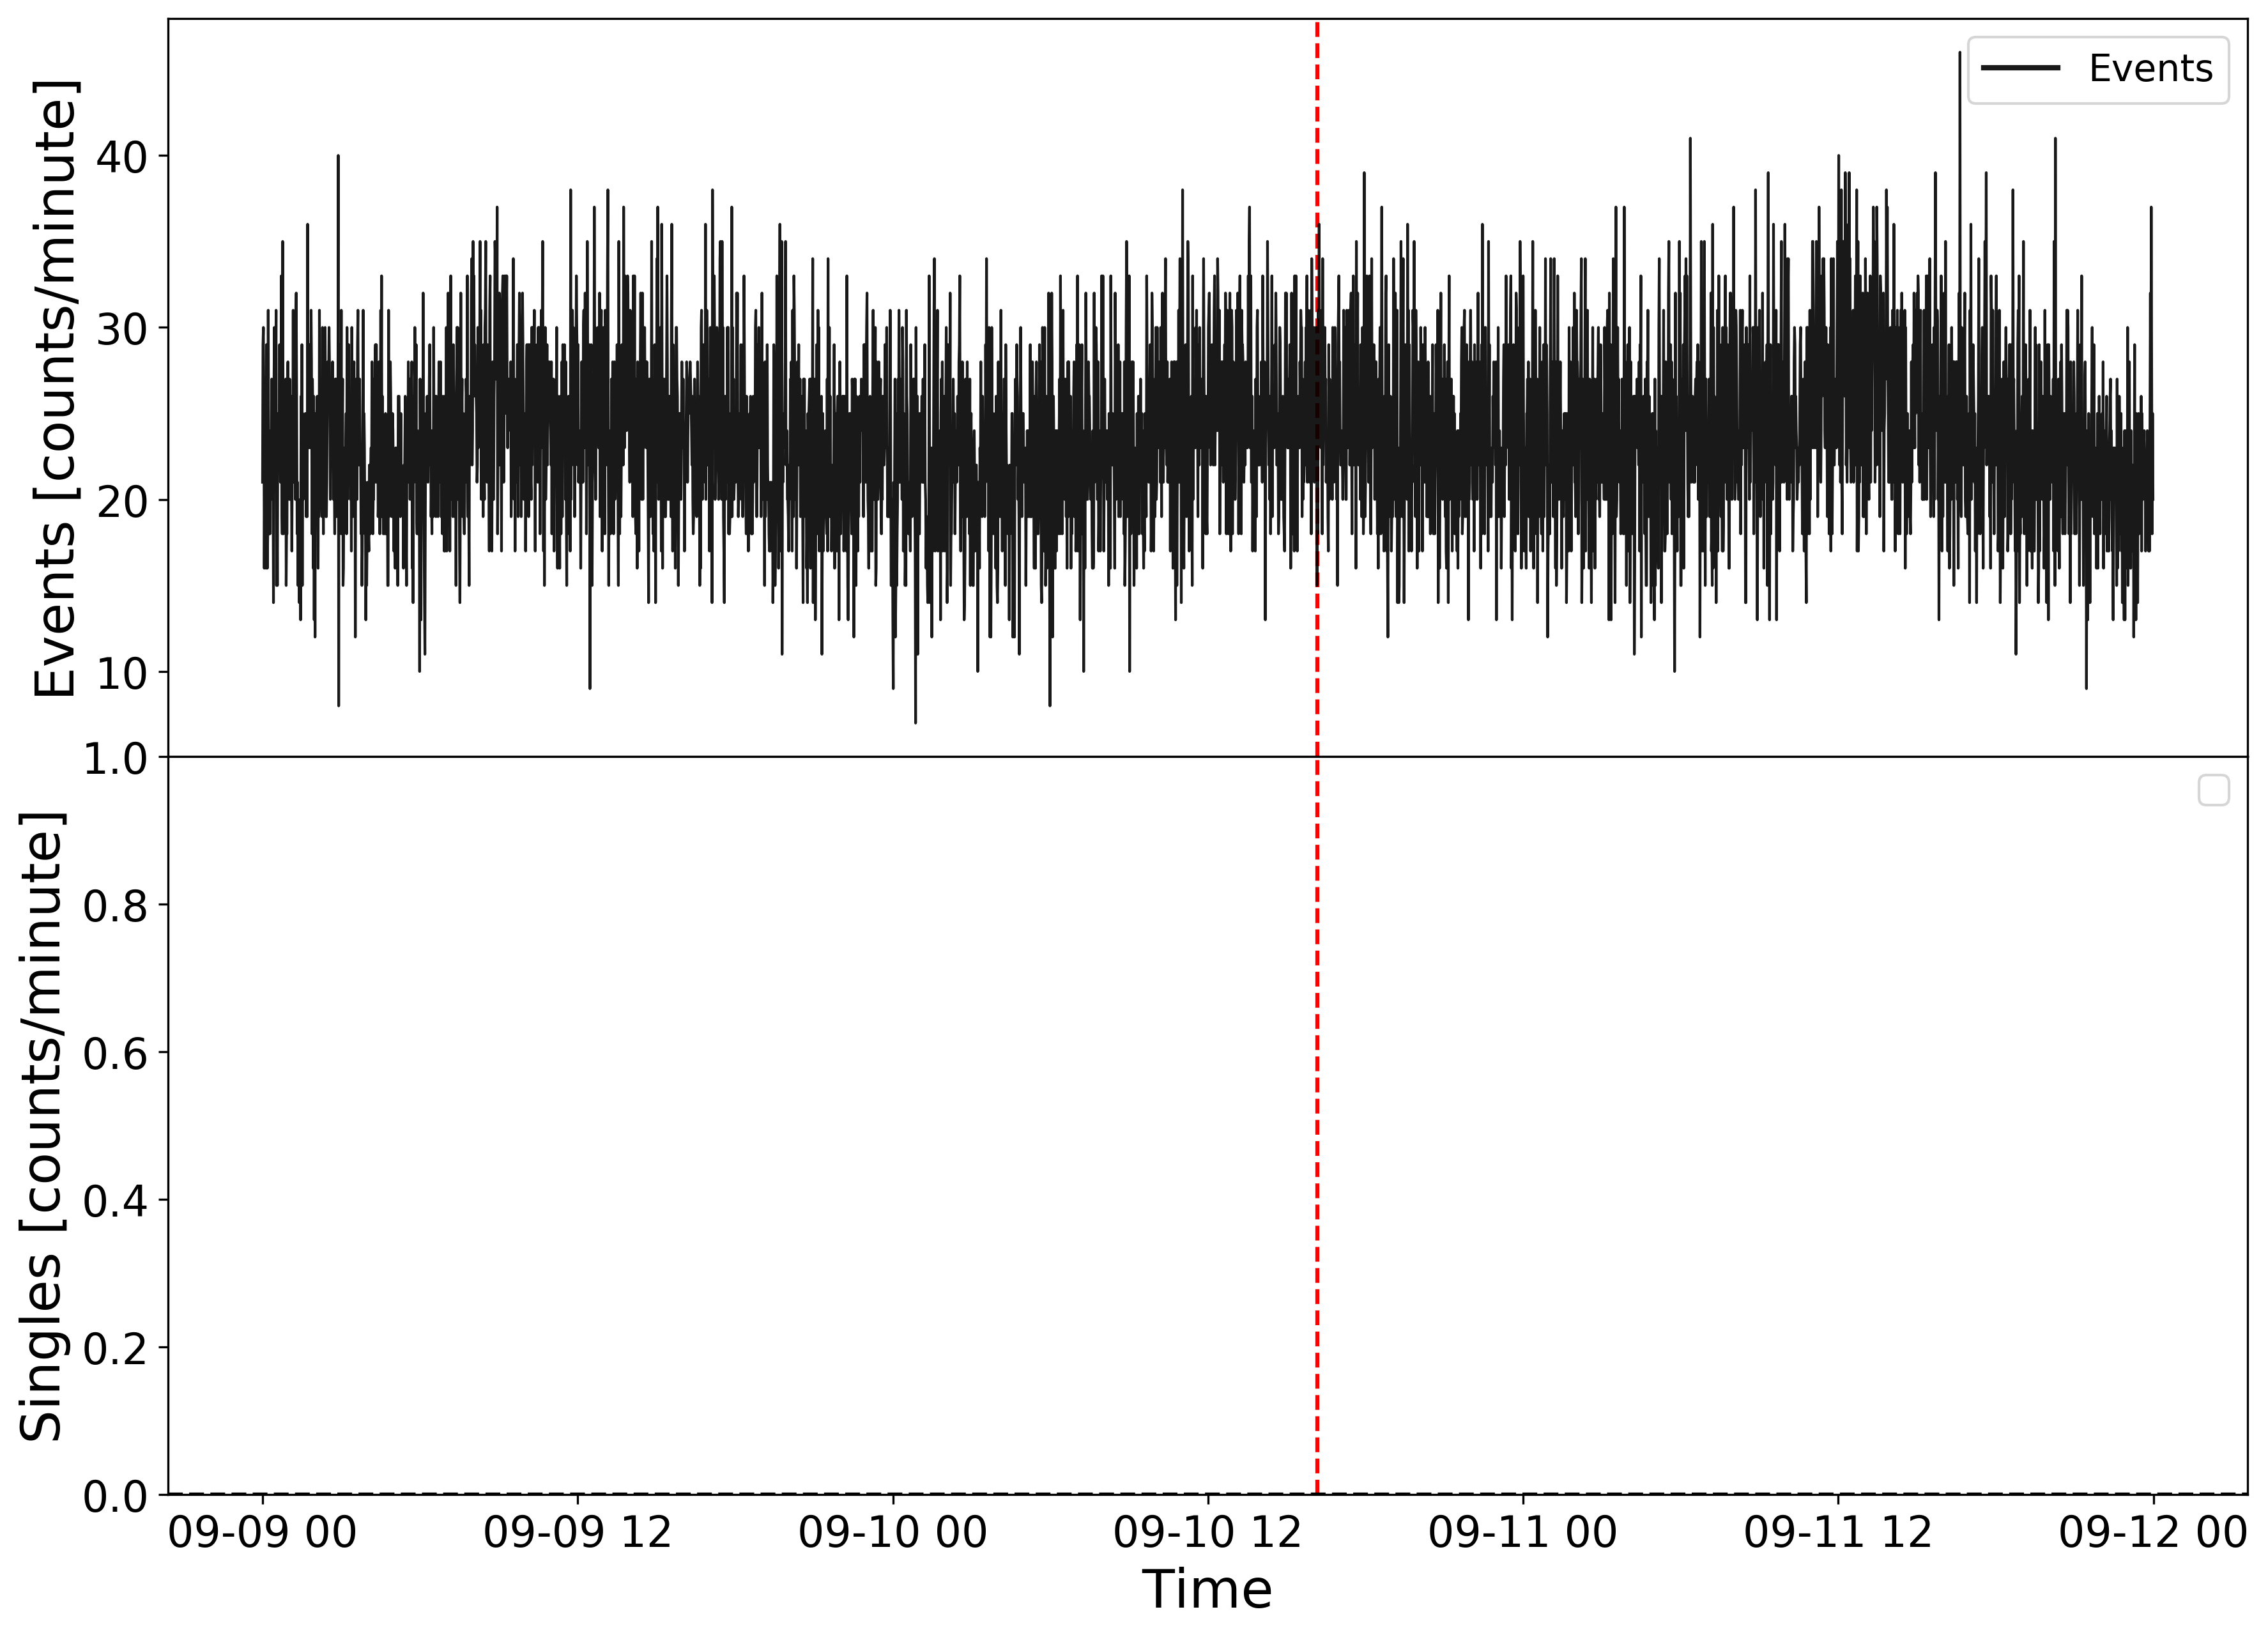
\includegraphics[width=0.48\columnwidth]{GLE72_14001.png}
		\label{fig:GLE72_14001}}
	
	\caption{HiSPARC data for 4 stations around the epoch of GLE 72. The top panel of each subplot shows the minute-averaged trigger events between detectors within the station, while the bottom panel shows the mean-shifted, minute-averaged counts by each individual detector in the station. The vertical red, dashed line depicts the approximate onset time of the GLE.}
	\label{fig:GLE_72}
\end{figure}

... no clear GLE seen...

%%%%%%%%%%%%%%%%%%%%%%%%%%%%%%%%%%%%%%%%%%%%%%%%%%%%%%%%%%%%%%%%%%%%%
\subsection{HiSPARC Observations of Forbush Decreases}

Figure~\ref{fig:FD_201203}...

\begin{figure}[ht]
	\centering
	\subfloat[HS 501 (Nikhef)]{
		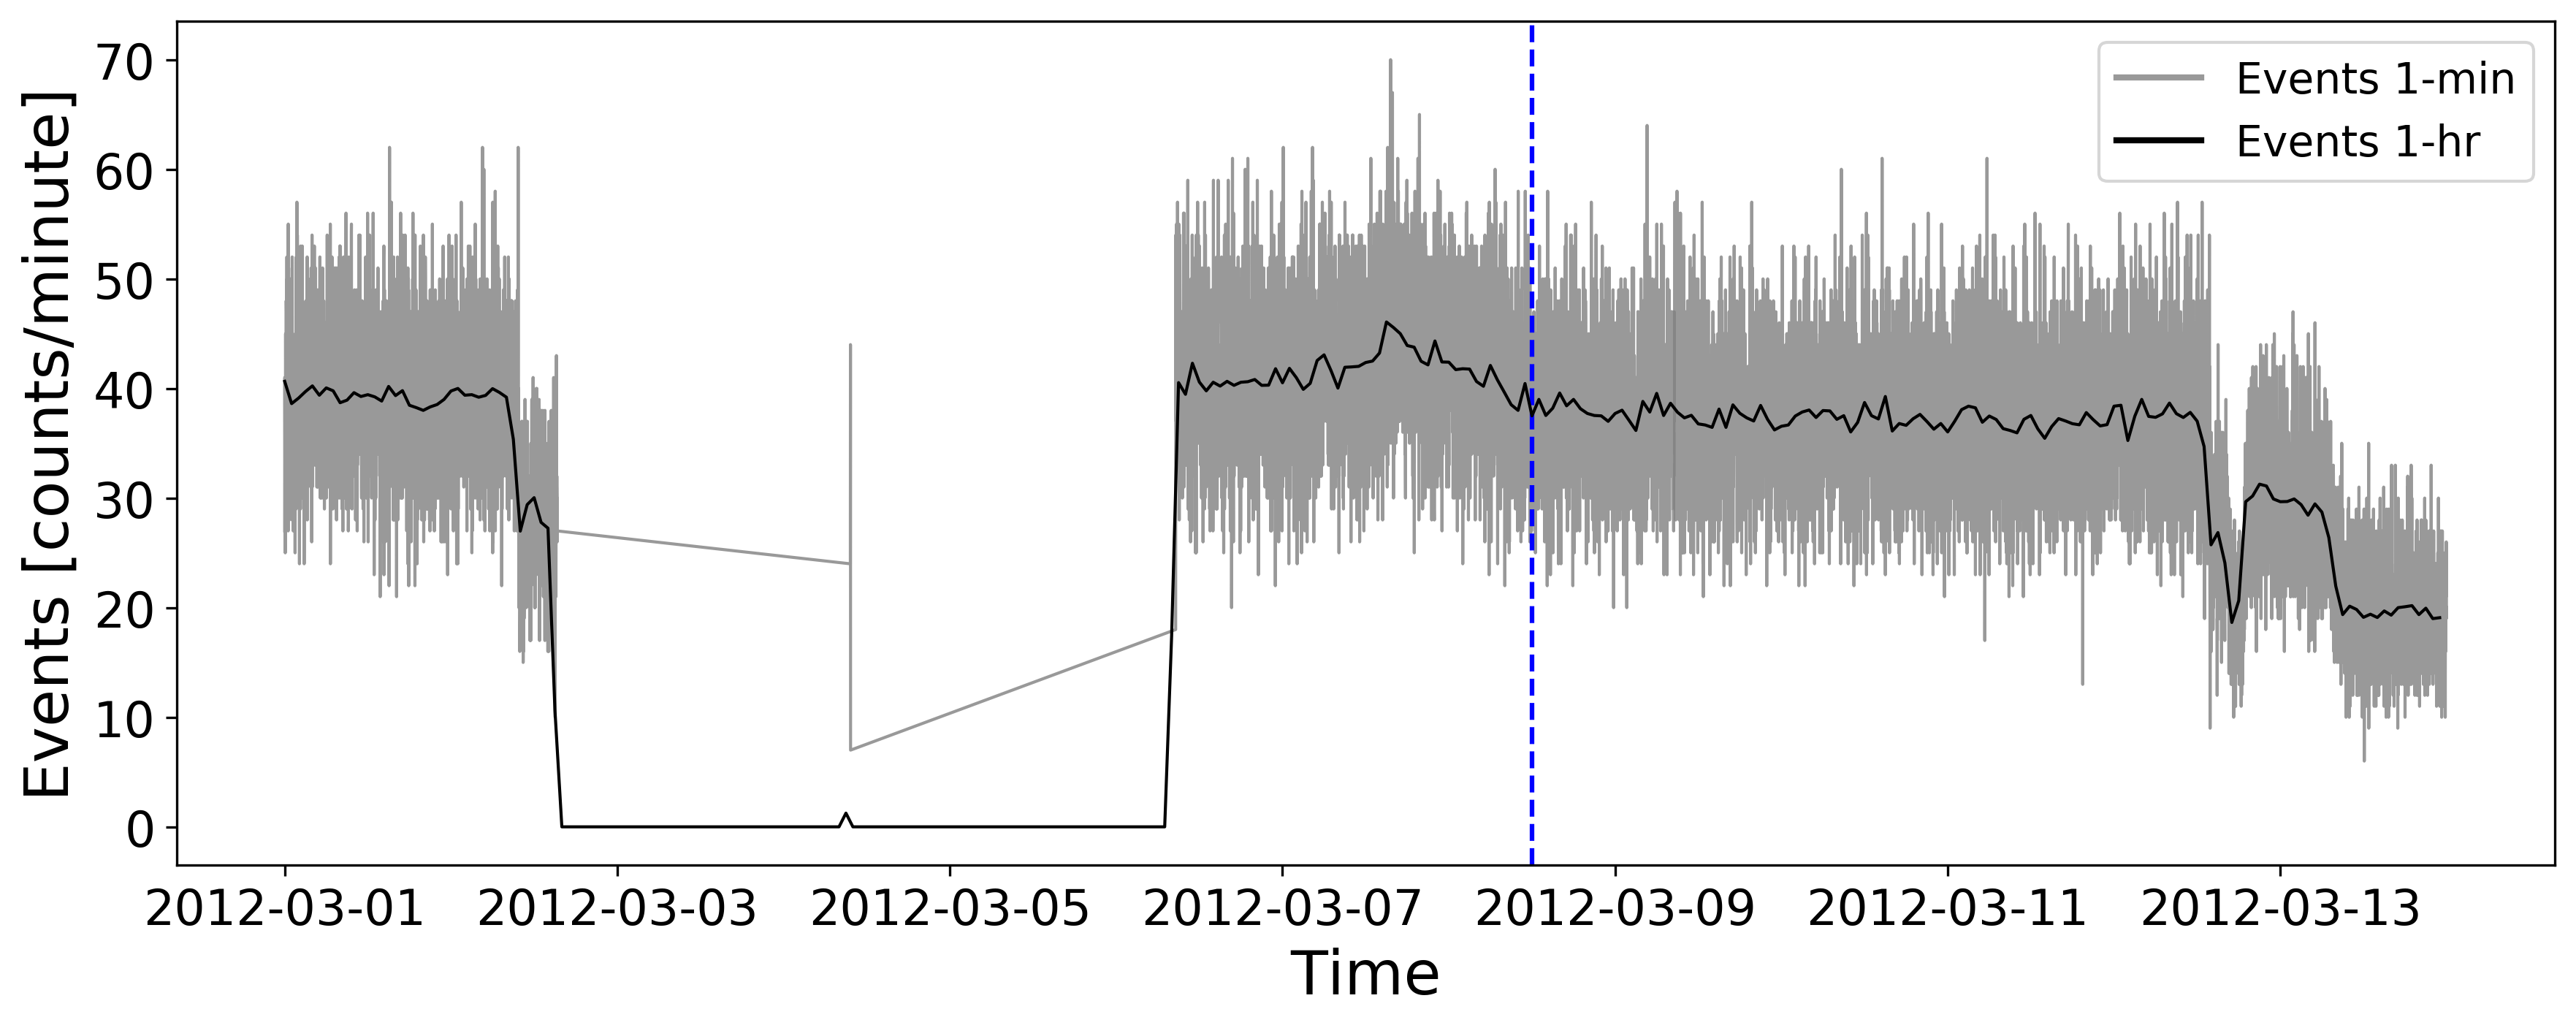
\includegraphics[width=0.48\columnwidth]{FD_201203_501.png}
		\label{fig:FD_201203_501}}
	%\qquad
	\subfloat[HS 8001 (Eindhoven)]{
		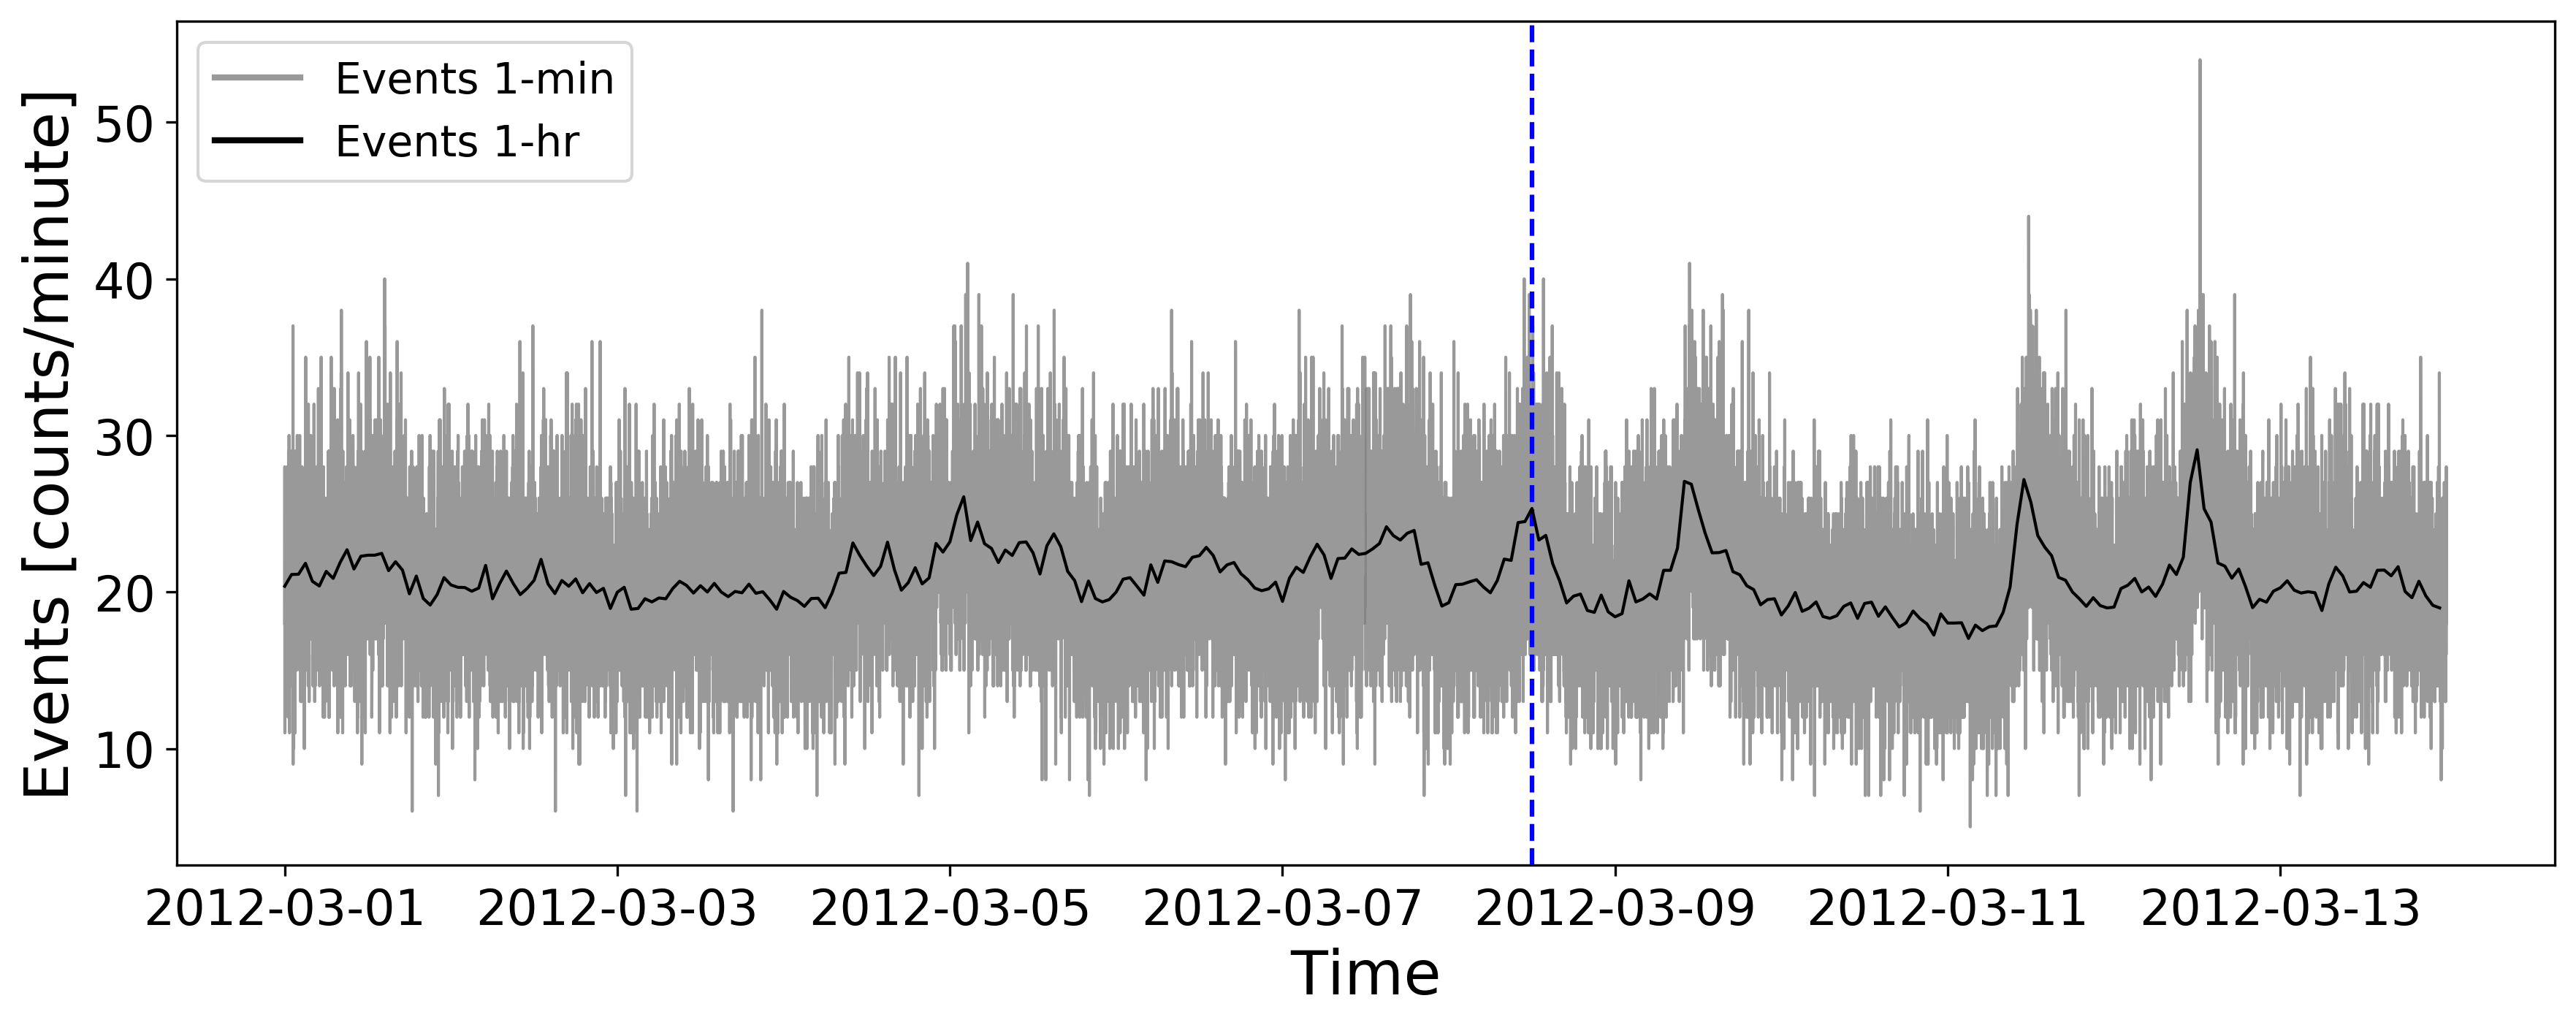
\includegraphics[width=0.48\columnwidth]{FD_201203_8001.png}
		\label{fig:FD_201203_8001}}
	
	\caption{HiSPARC data for stations 501 and 8001 around the epoch of the FD in March 2012. The plot shows the minute-averaged and hourly-averaged trigger events between detectors within the station. The vertical blue-dashed line shows the approximate onset-time of the FD.}
	\label{fig:FD_201203}
\end{figure}


Figure~\ref{fig:FD_201207}...

\begin{figure}[ht]
	\centering
	\subfloat[HS 501 (Nikhef)]{
		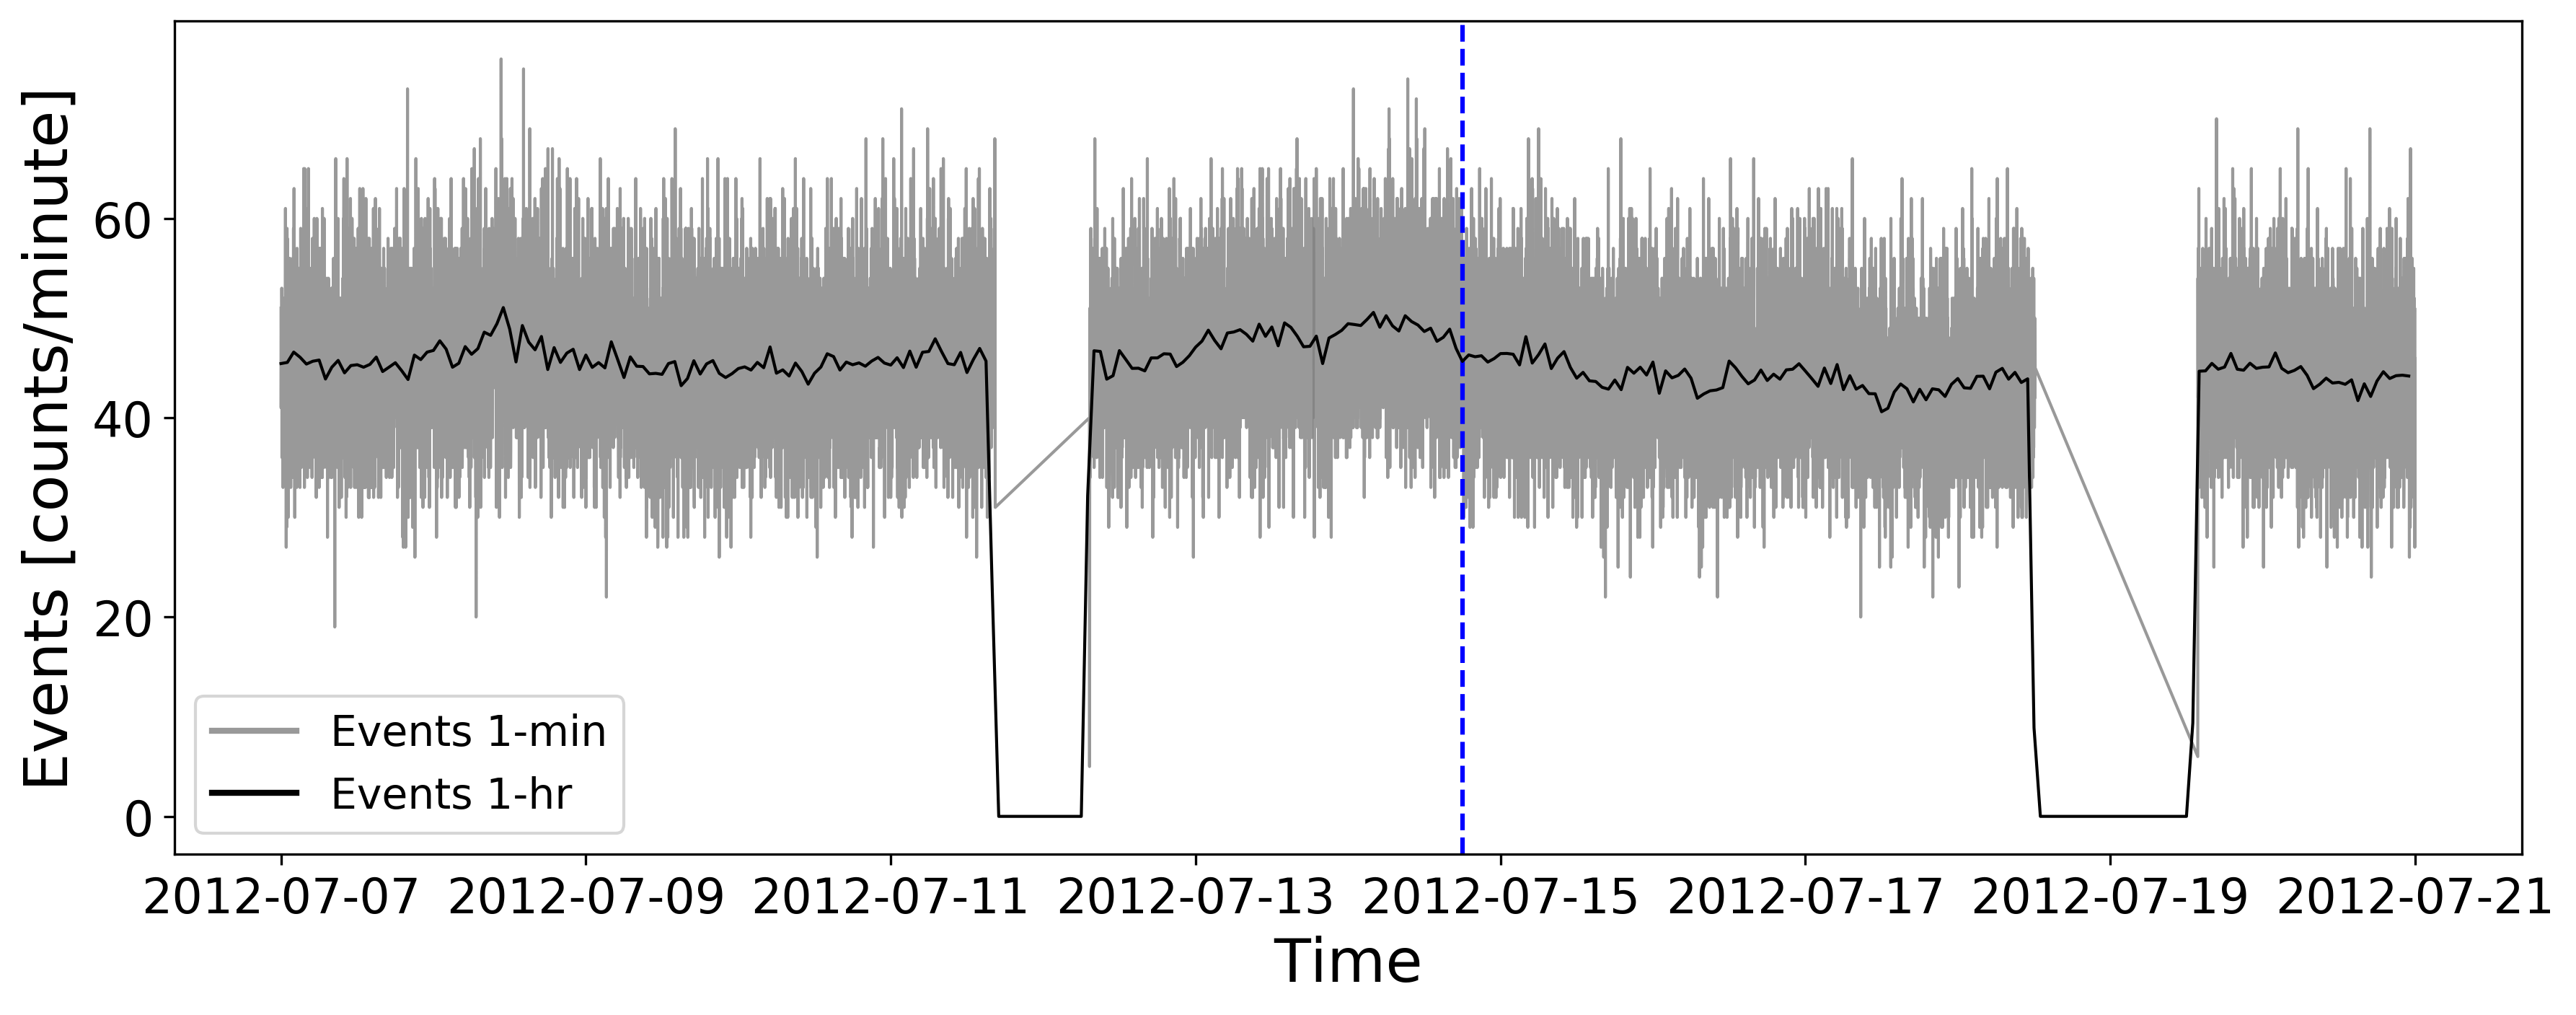
\includegraphics[width=0.48\columnwidth]{FD_201207_501.png}
		\label{fig:FD_201207_501}}
	%\qquad
	\subfloat[HS 8001 (Eindhoven)]{
		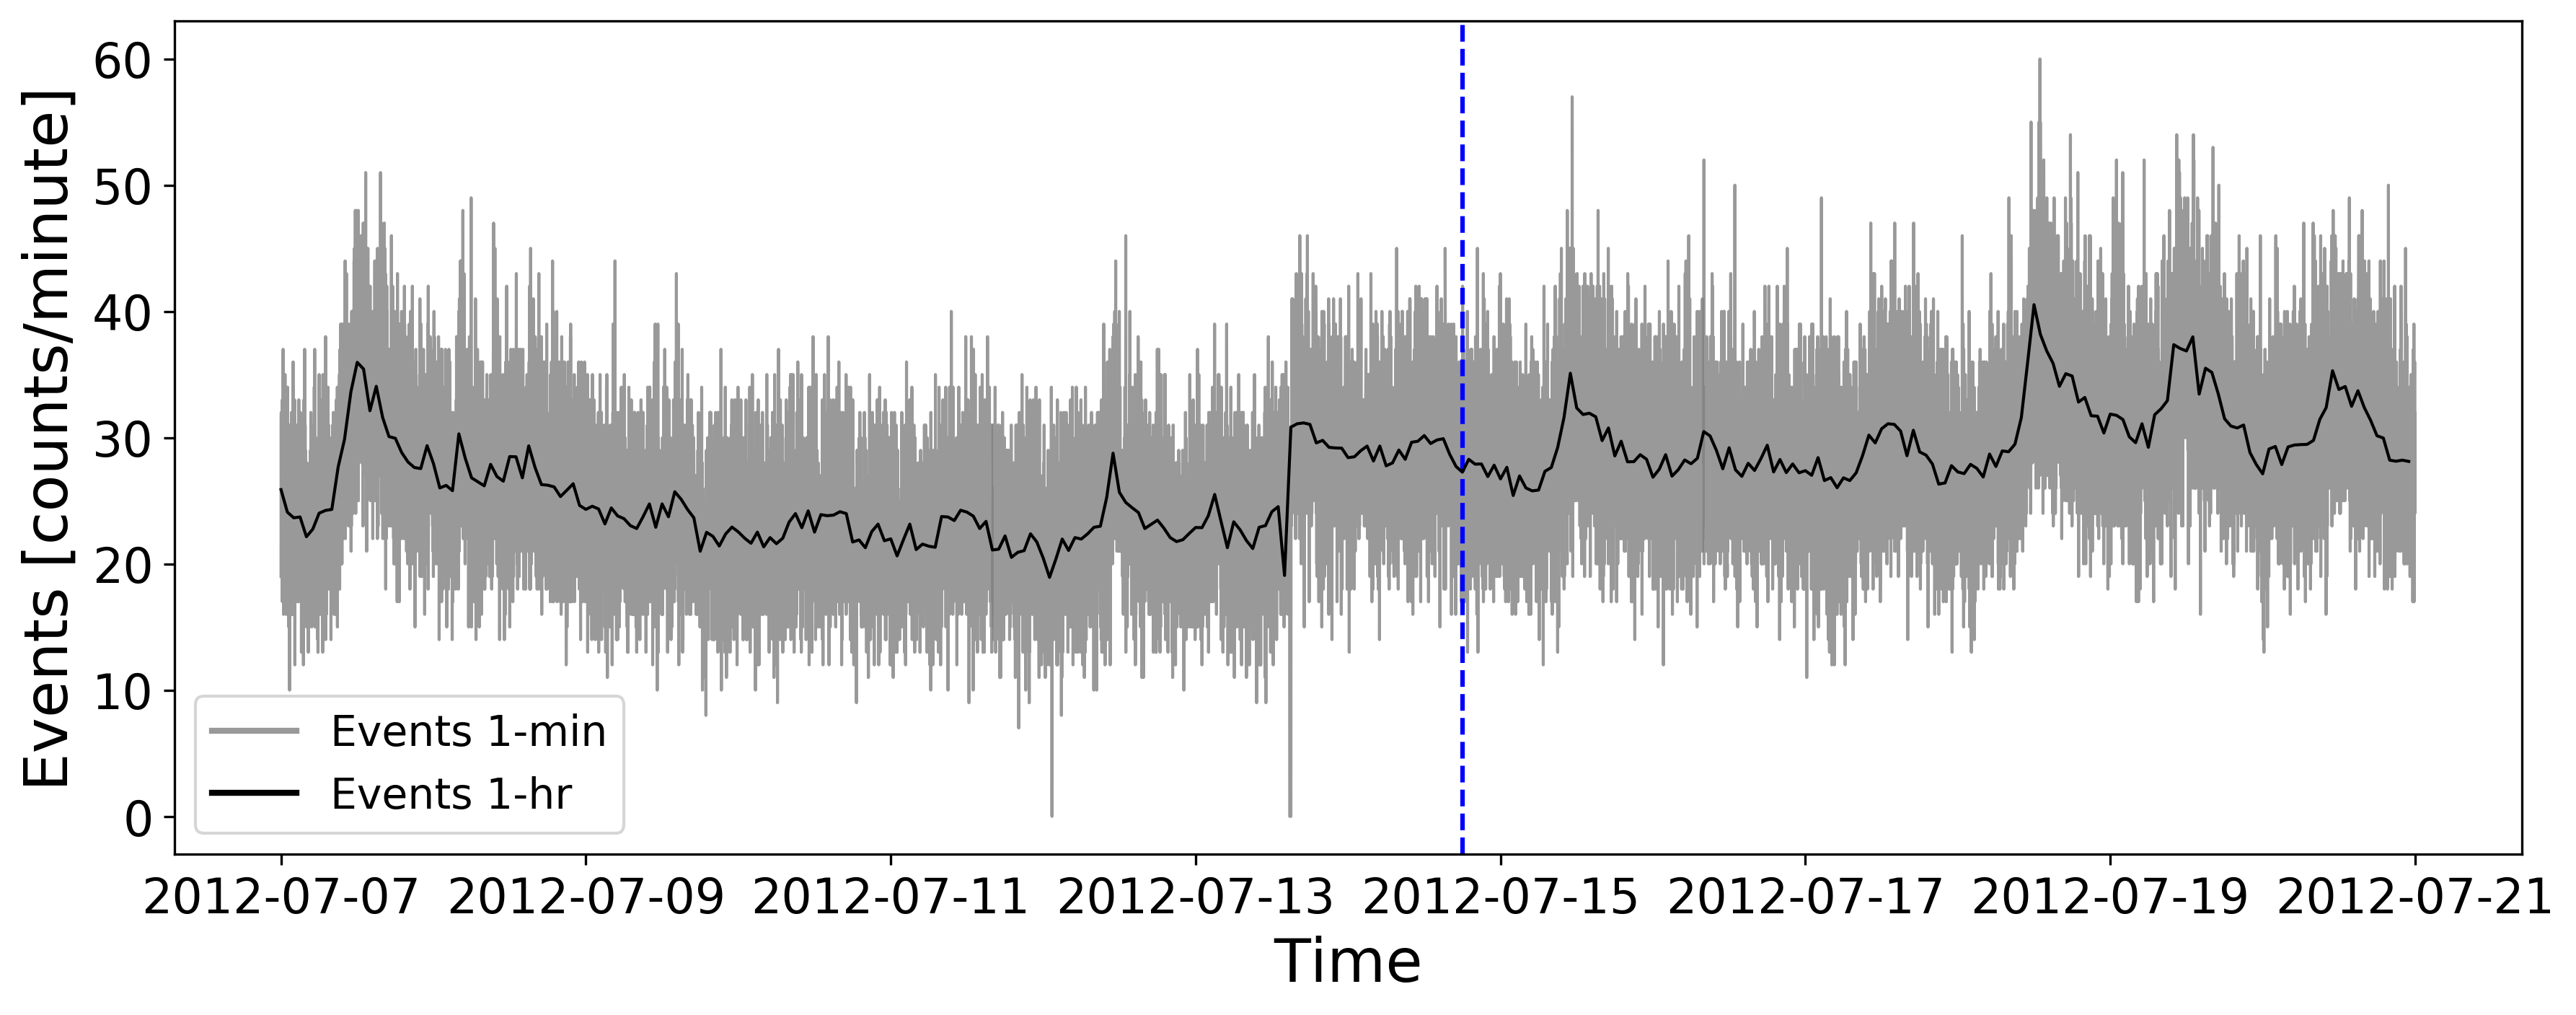
\includegraphics[width=0.48\columnwidth]{FD_201207_8001.png}
		\label{fig:FD_201207_8001}}
	
	\caption{HiSPARC data for stations 501 and 8001 around the epoch of the FD in July 2012. The plot shows the minute-averaged and hourly-averaged trigger events between detectors within the station. The vertical blue-dashed line shows the approximate onset-time of the FD.}
	\label{fig:FD_201207}
\end{figure}



Figure~\ref{fig:FD_201412}...

\begin{figure}[ht]
	\centering
	\subfloat[HS 501 (Nikhef)]{
		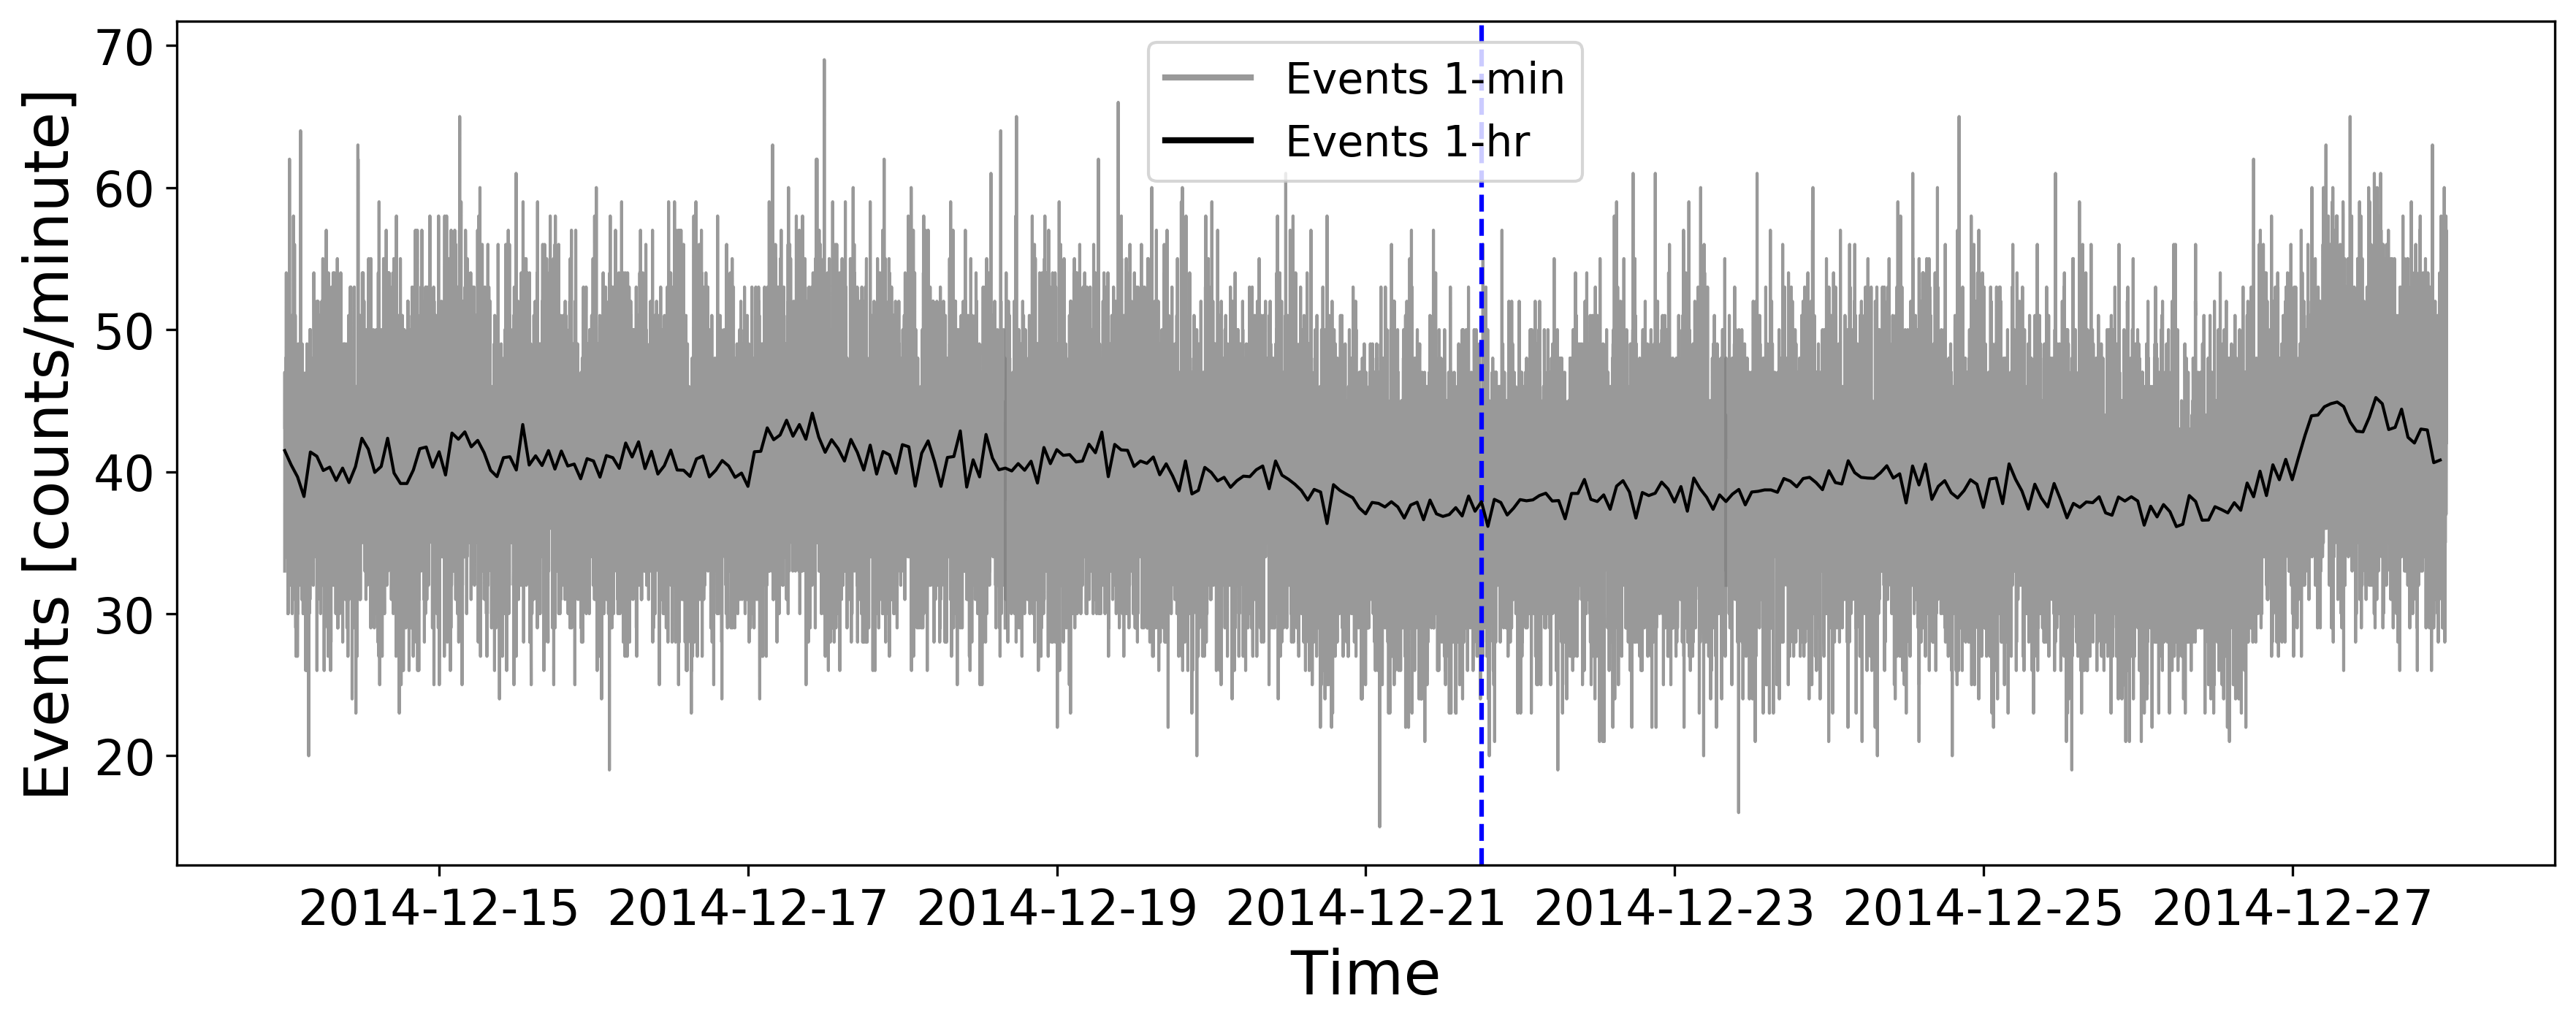
\includegraphics[width=0.48\columnwidth]{FD_201412_501.png}
		\label{fig:FD_201412_501}}
	%\qquad
	\subfloat[HS 203 (College Hageveld)]{
		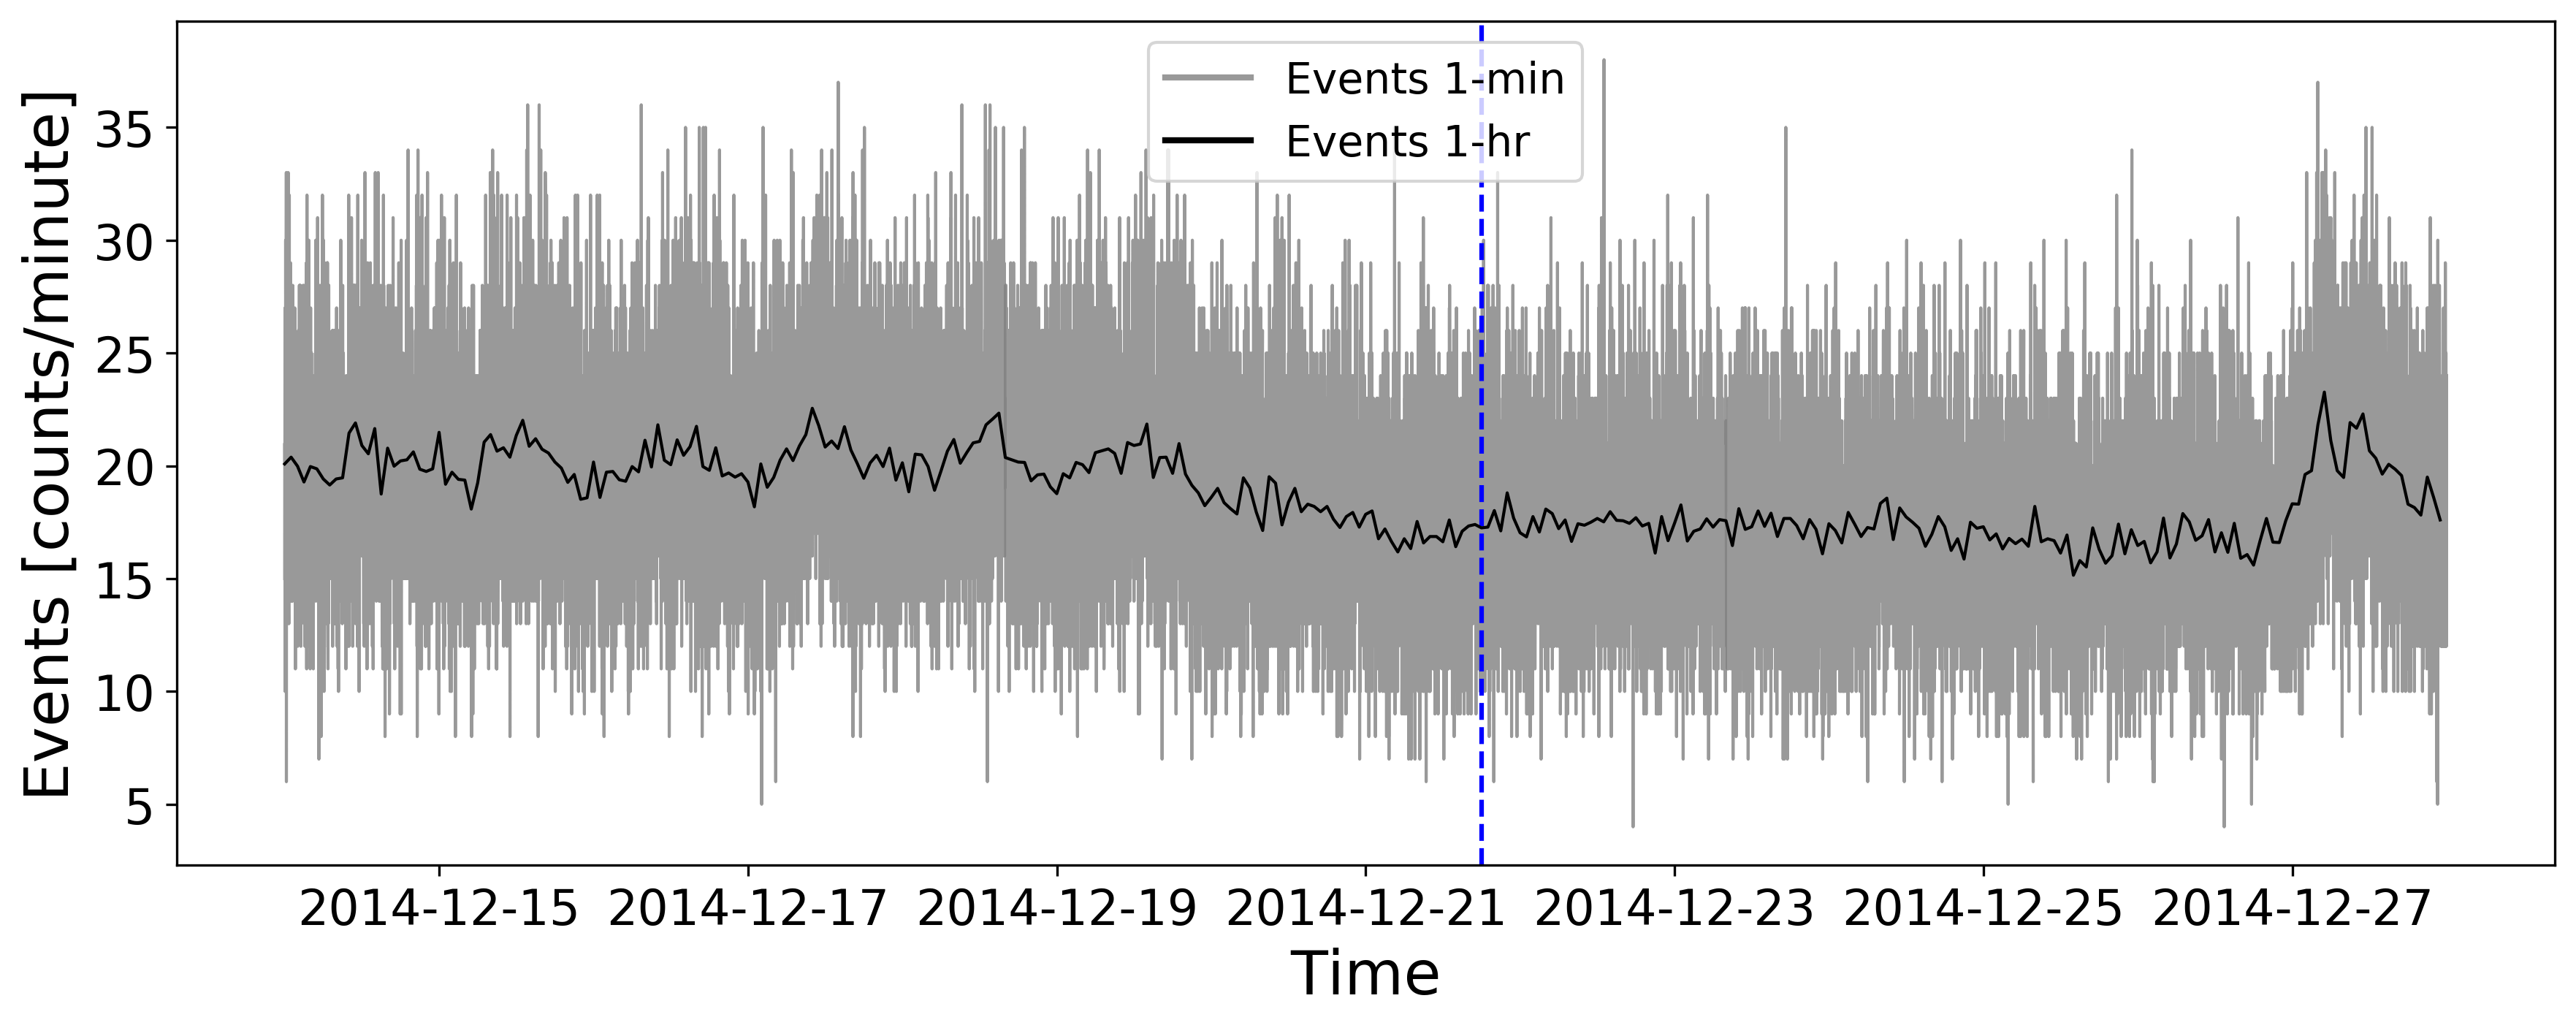
\includegraphics[width=0.48\columnwidth]{FD_201412_203.png}
		\label{fig:FD_201412_203}} \\
	
	\qquad
	
	\subfloat[HS 3001 (Leiden)]{
		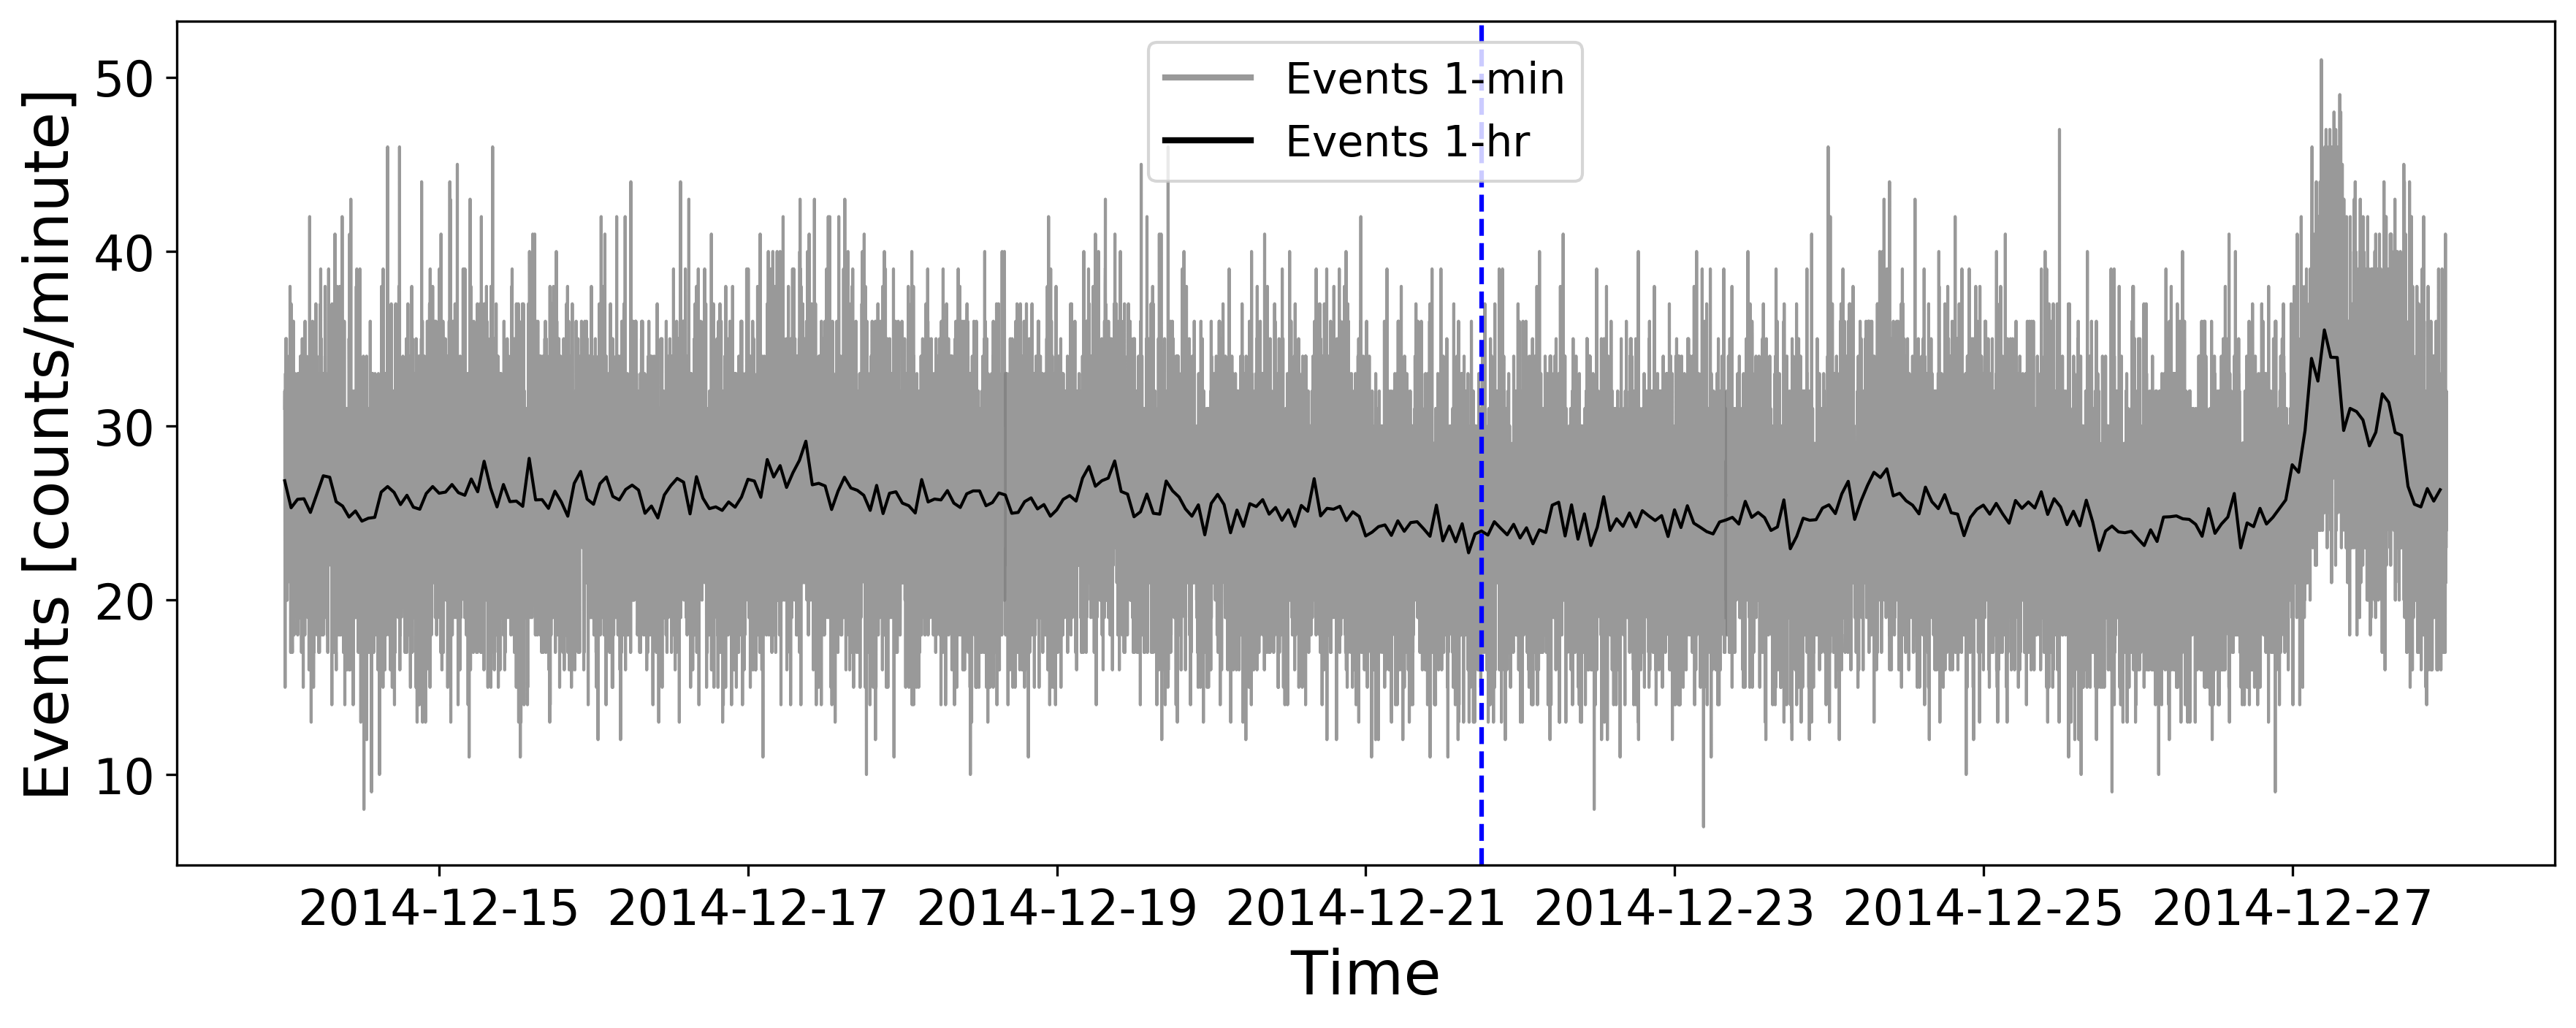
\includegraphics[width=0.48\columnwidth]{FD_201412_3001.png}
		\label{fig:FD_201412_3001}}
	%\qquad
	\subfloat[HS 14001 (Birmingham University)]{
		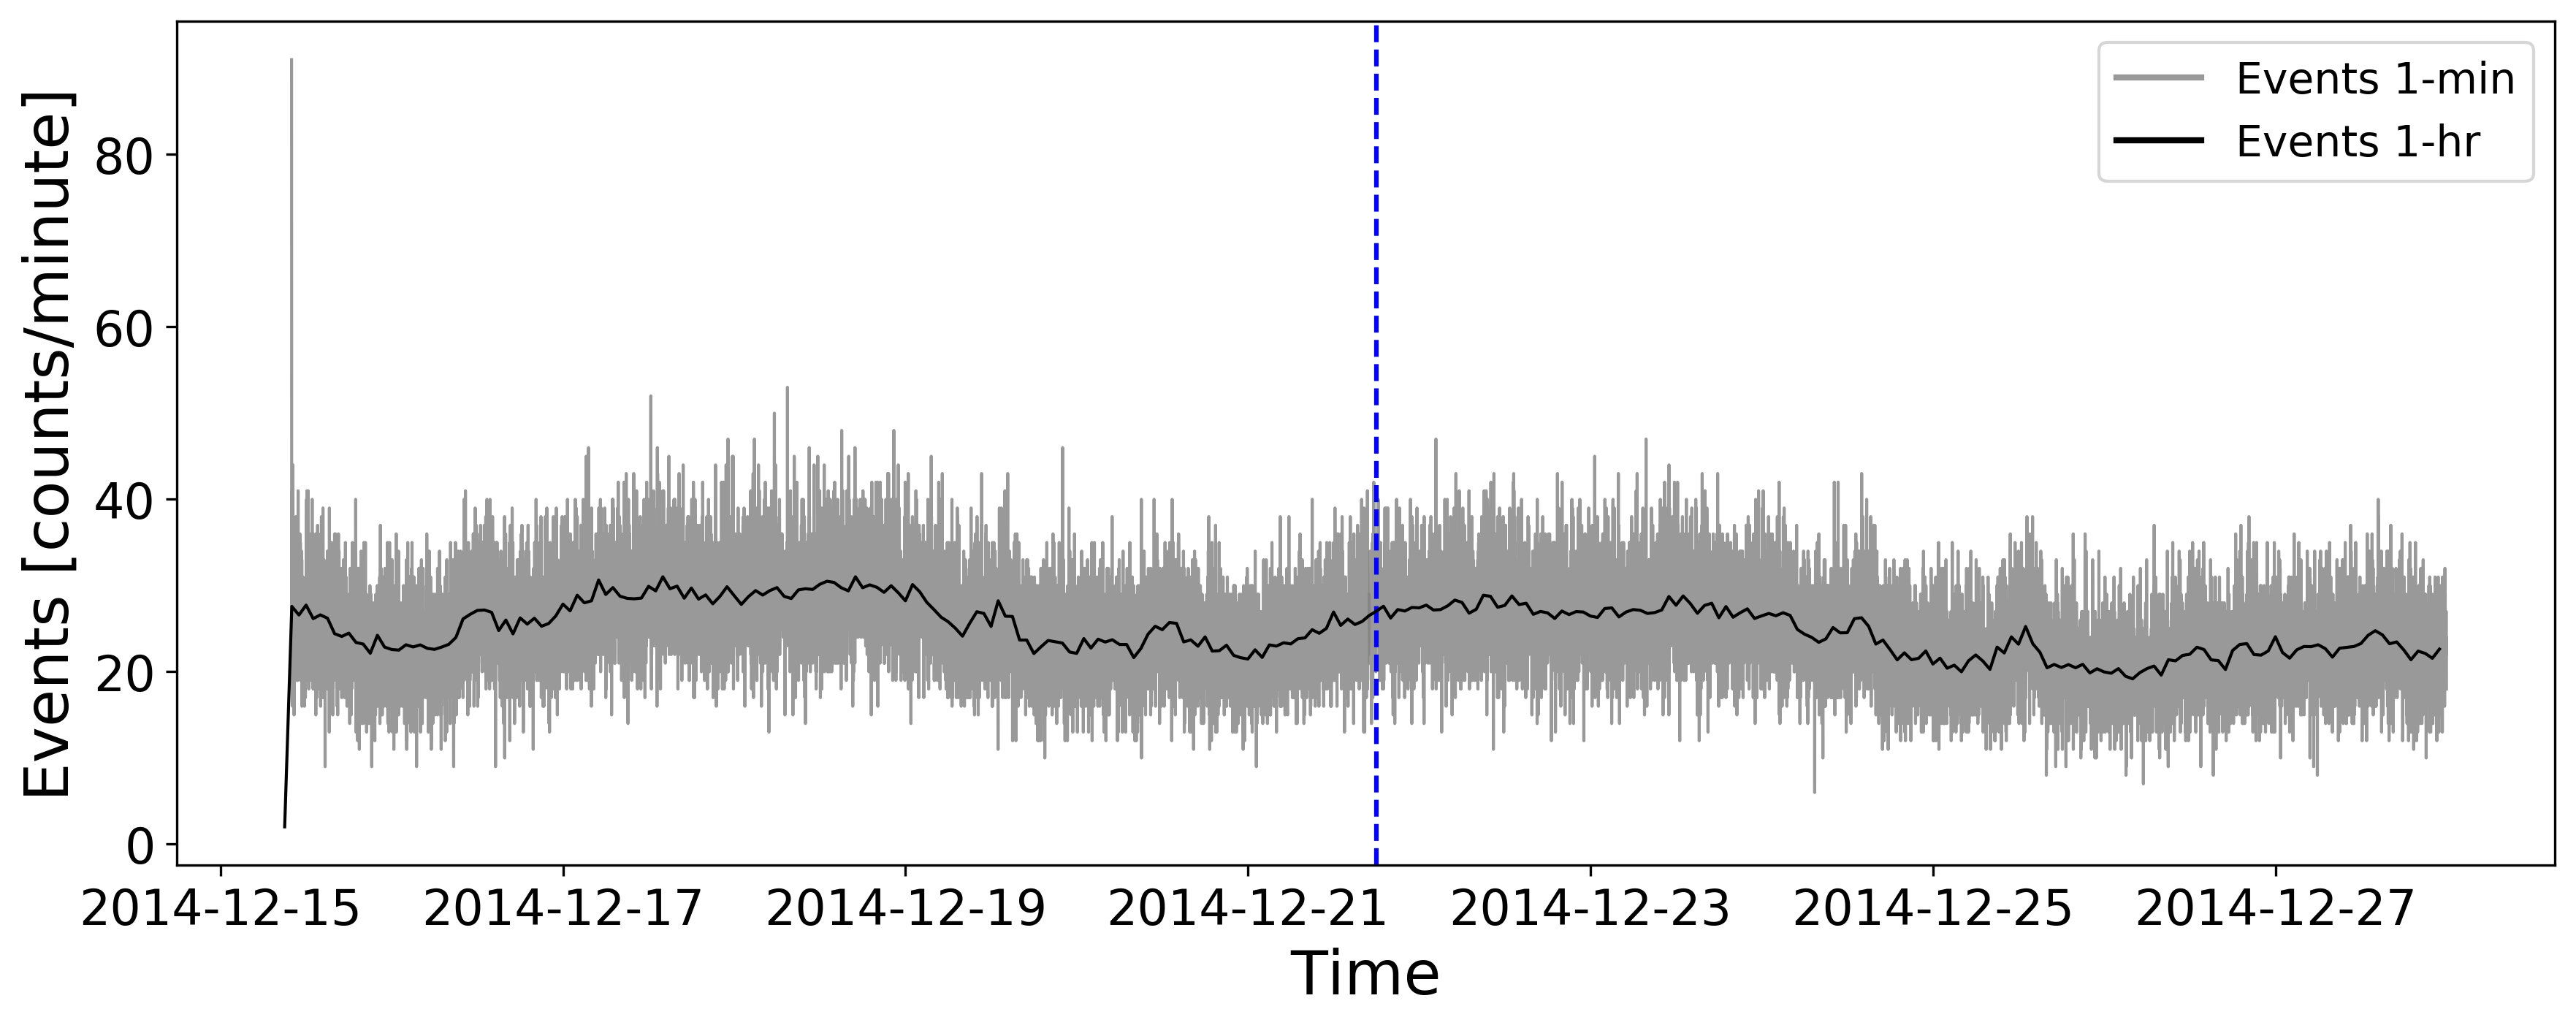
\includegraphics[width=0.48\columnwidth]{FD_201412_14001.png}
		\label{fig:FD_201412_14001}}
	
	\caption{HiSPARC data for 4 stations around the epoch of the FD in December 2014. The plot shows the minute-averaged and hourly-averaged trigger events between detectors within the station. The vertical blue-dashed line shows the approximate onset-time of the FD.}
	\label{fig:FD_201412}
\end{figure}



Figure~\ref{fig:FD_GLE72}...

\begin{figure}[ht]
	\centering
	\subfloat[HS 501 (Nikhef)]{
		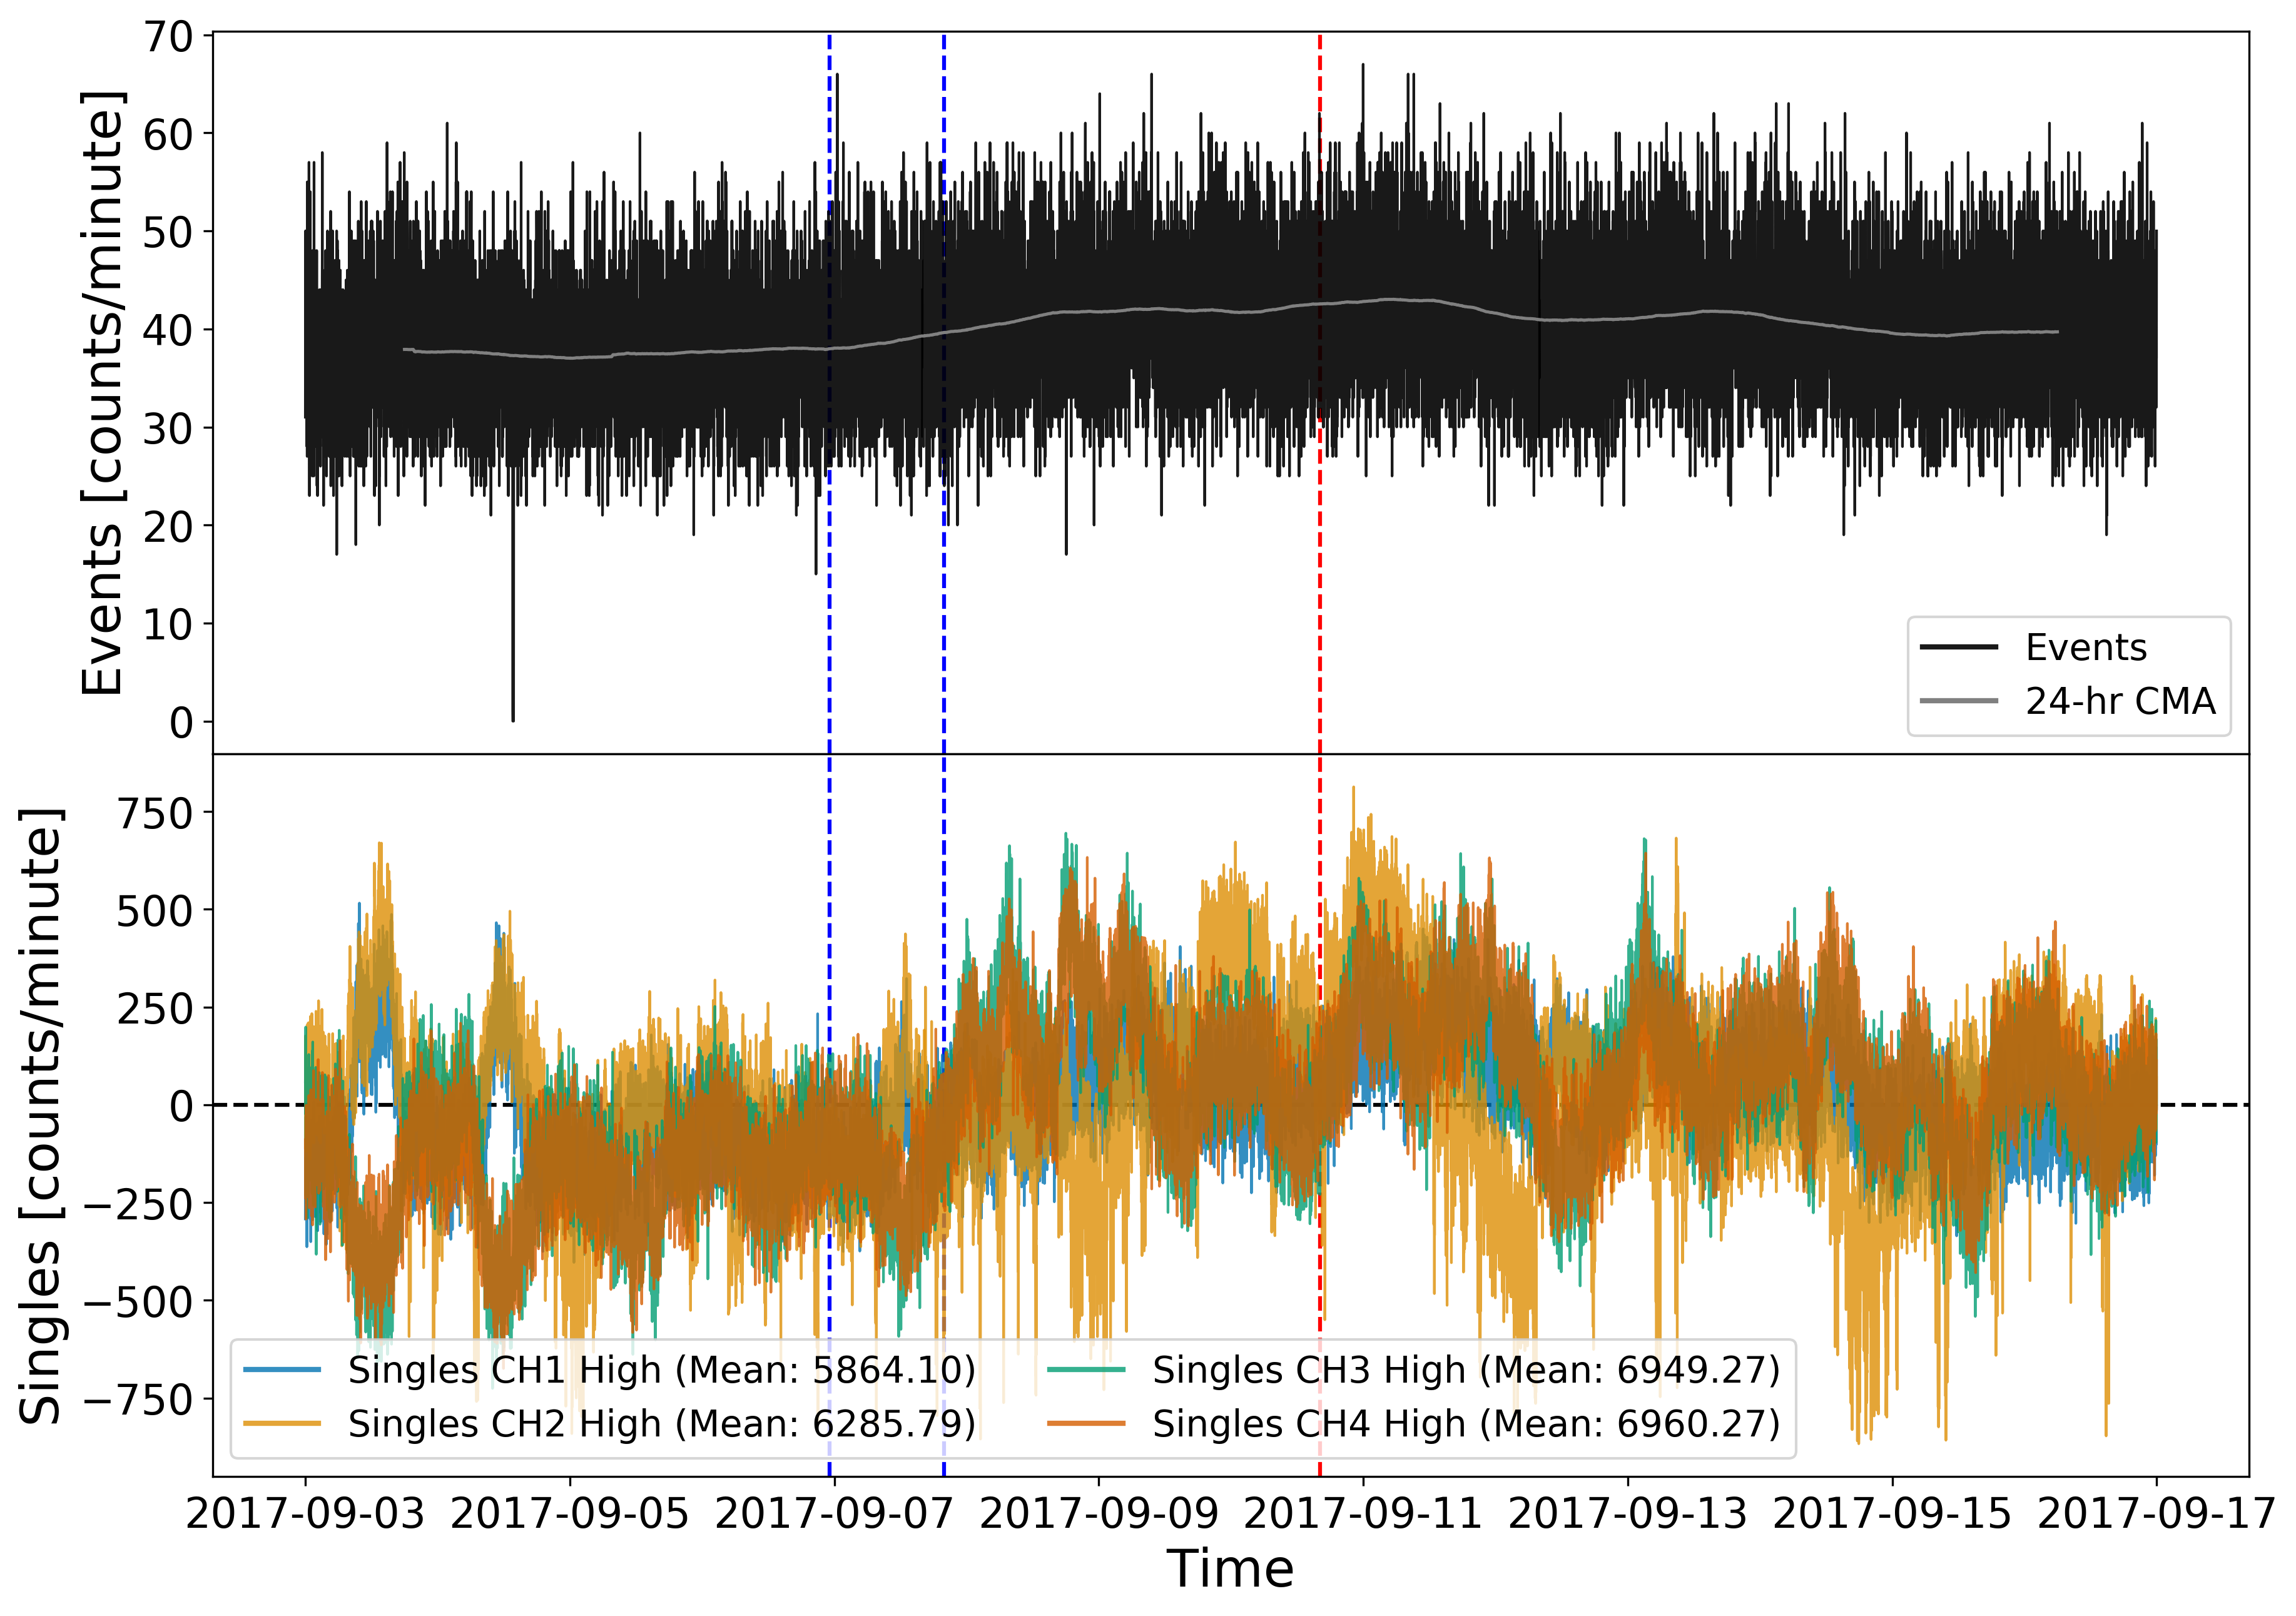
\includegraphics[width=0.48\columnwidth]{FD_GLE72_501.png}
		\label{fig:FD_GLE72_501}}
	%\qquad
	\subfloat[HS 203 (College Hageveld)]{
		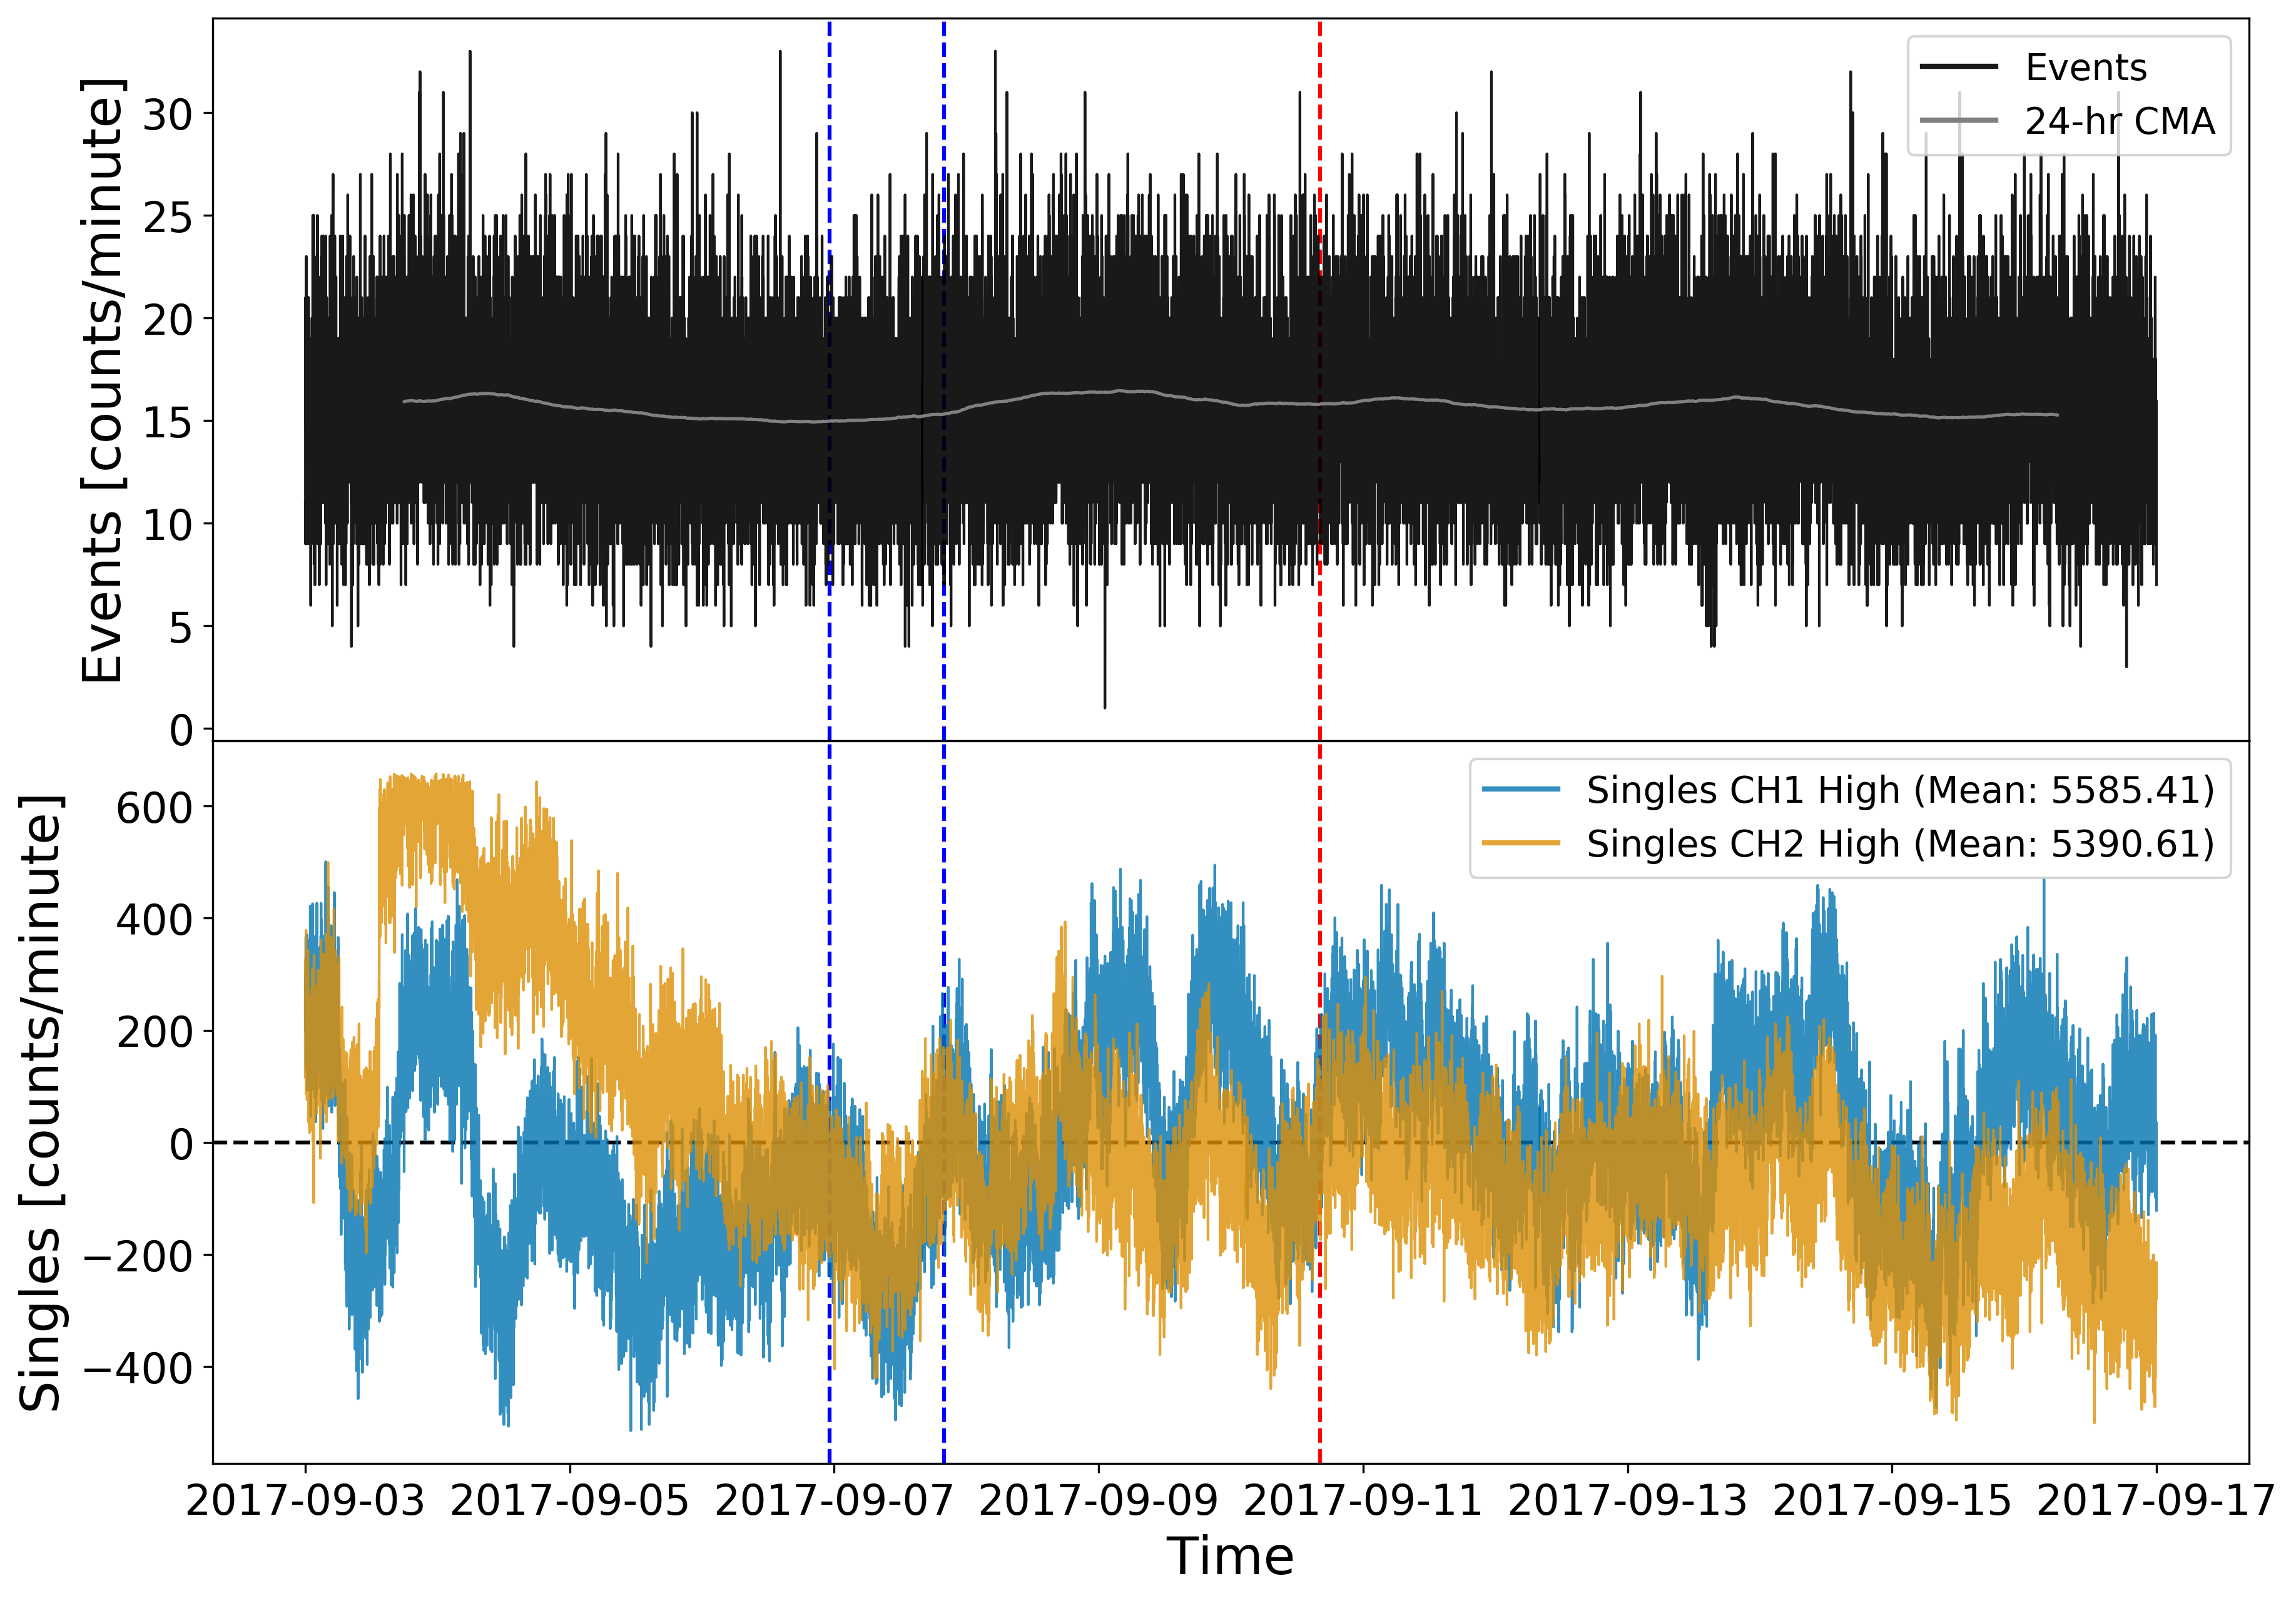
\includegraphics[width=0.48\columnwidth]{FD_GLE72_203.png}
		\label{fig:FD_GLE72_203}} \\
	
	\qquad
	
	\subfloat[HS 8001 (Eindhoven)]{
		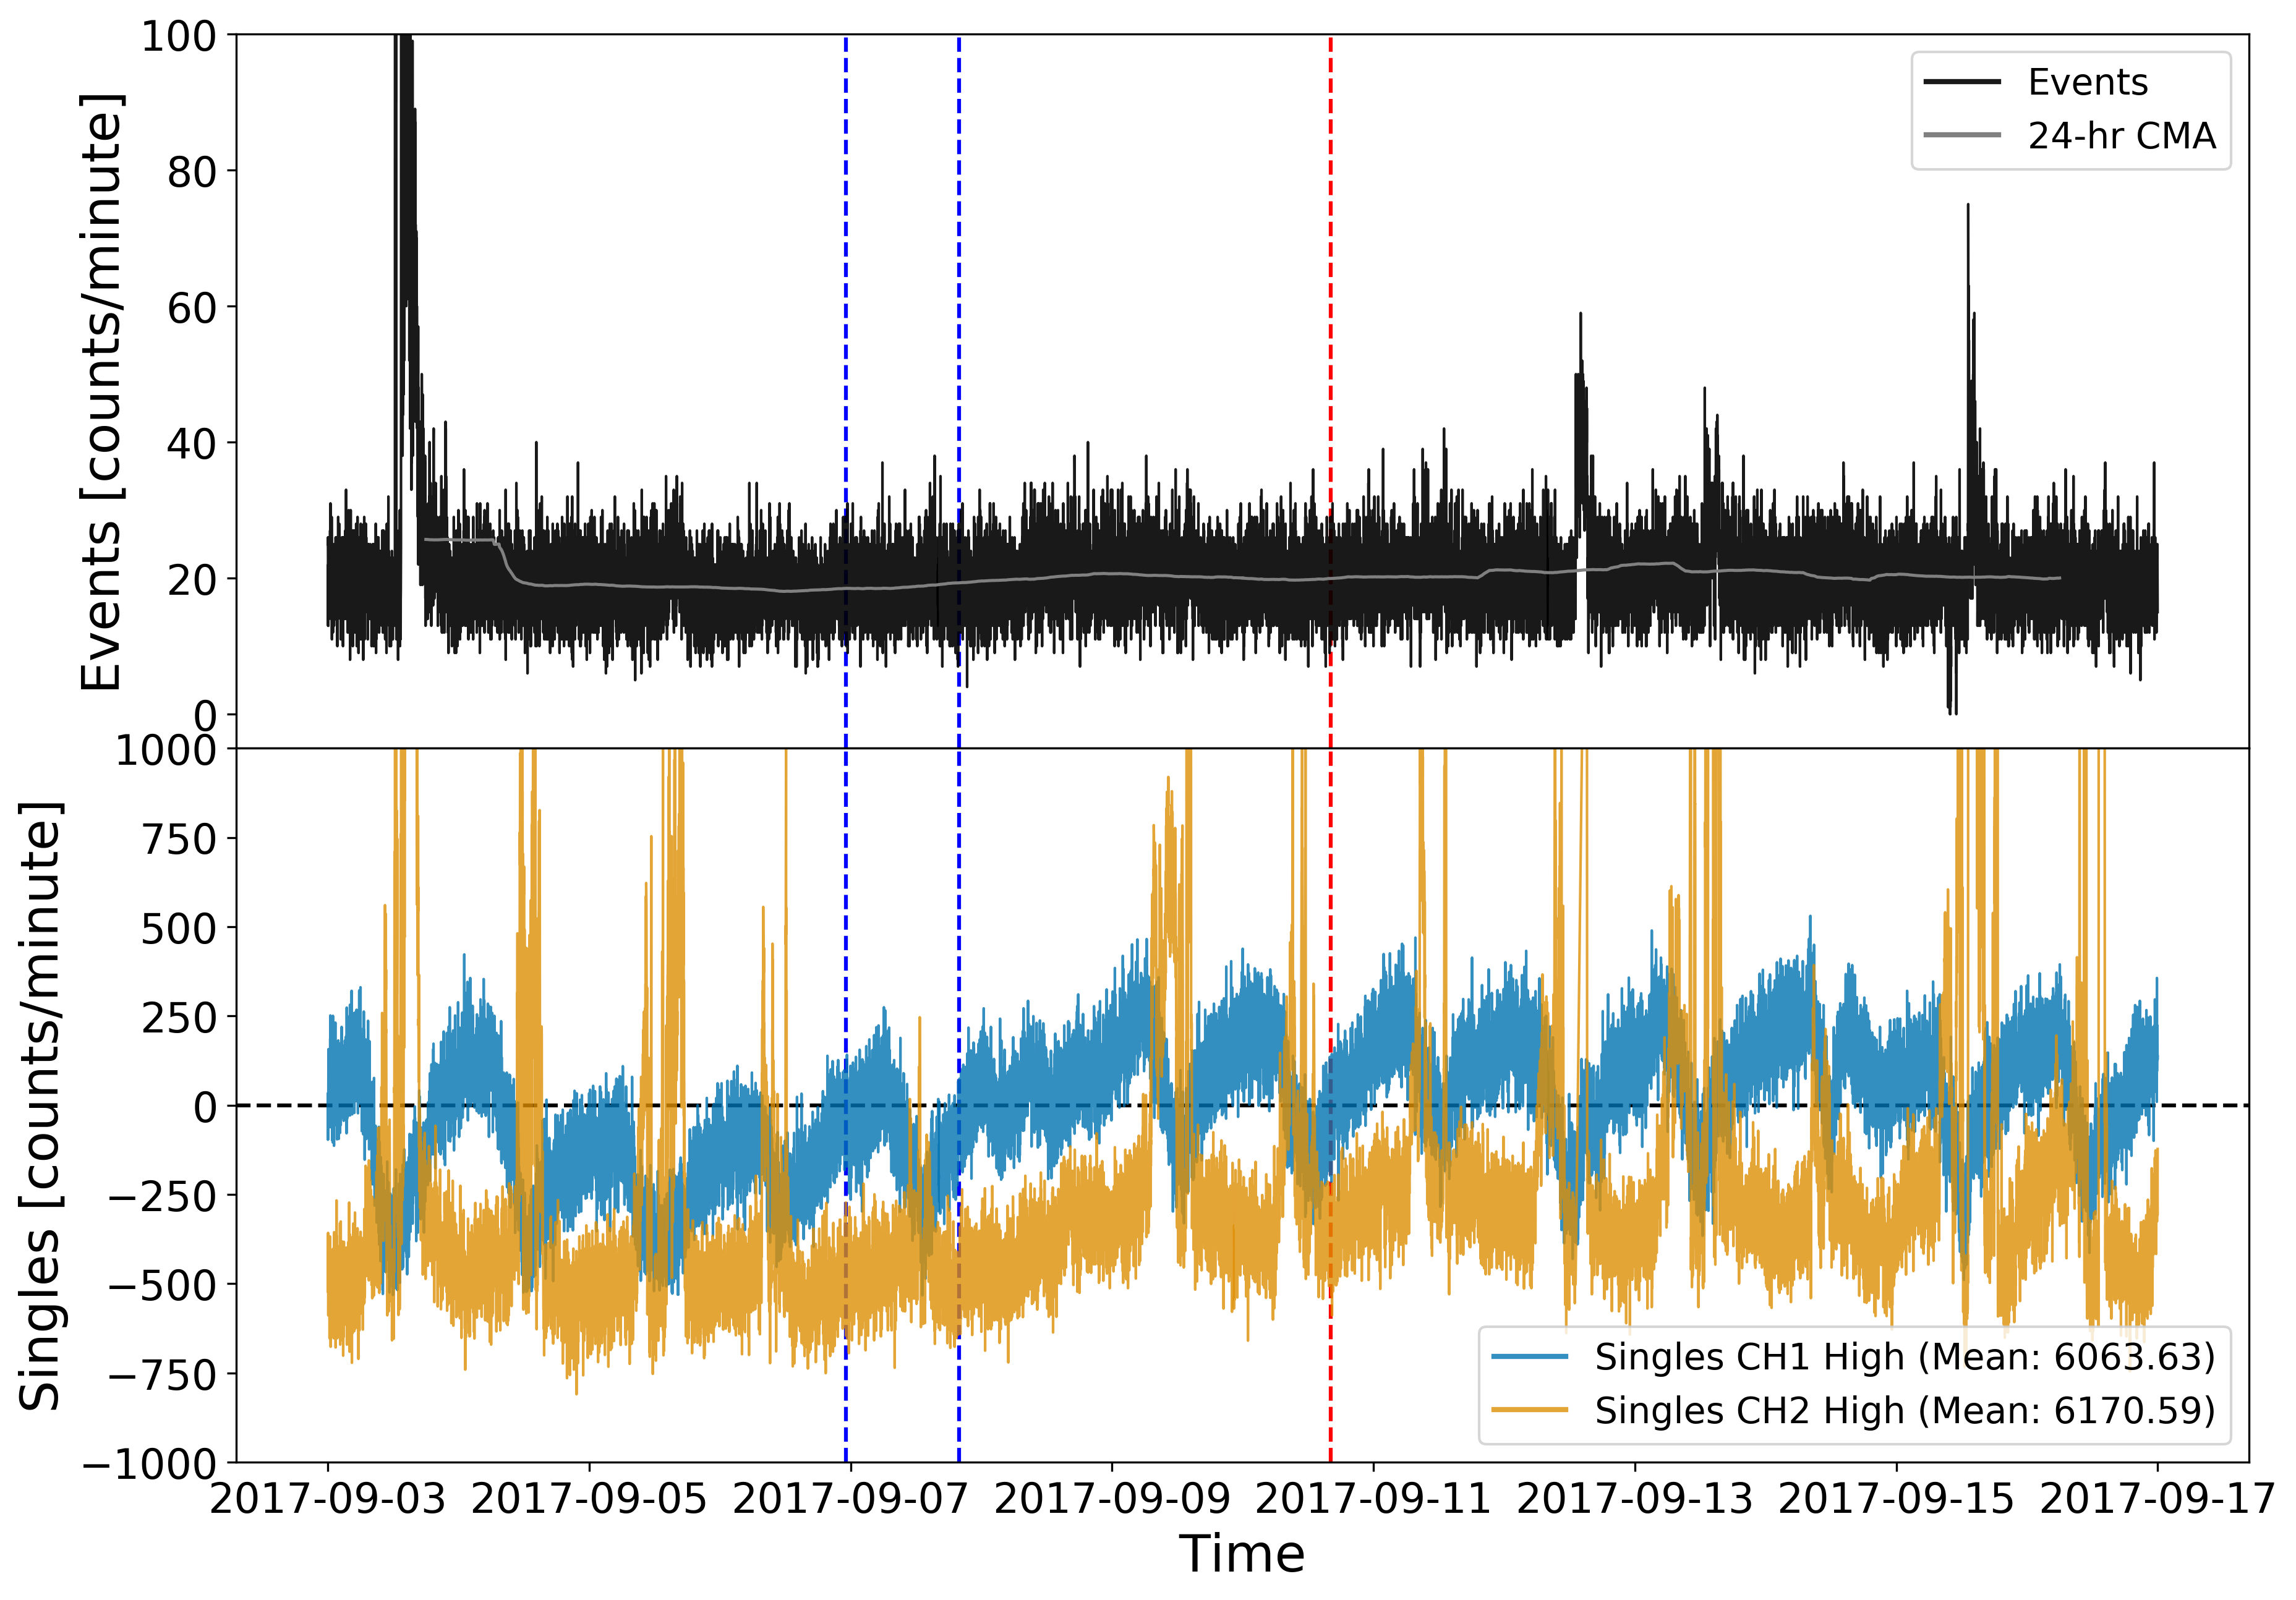
\includegraphics[width=0.48\columnwidth]{FD_GLE72_8001.png}
		\label{fig:FD_GLE72_8001}}
	%\qquad
	\subfloat[HS 14001 (Birmingham University)]{
		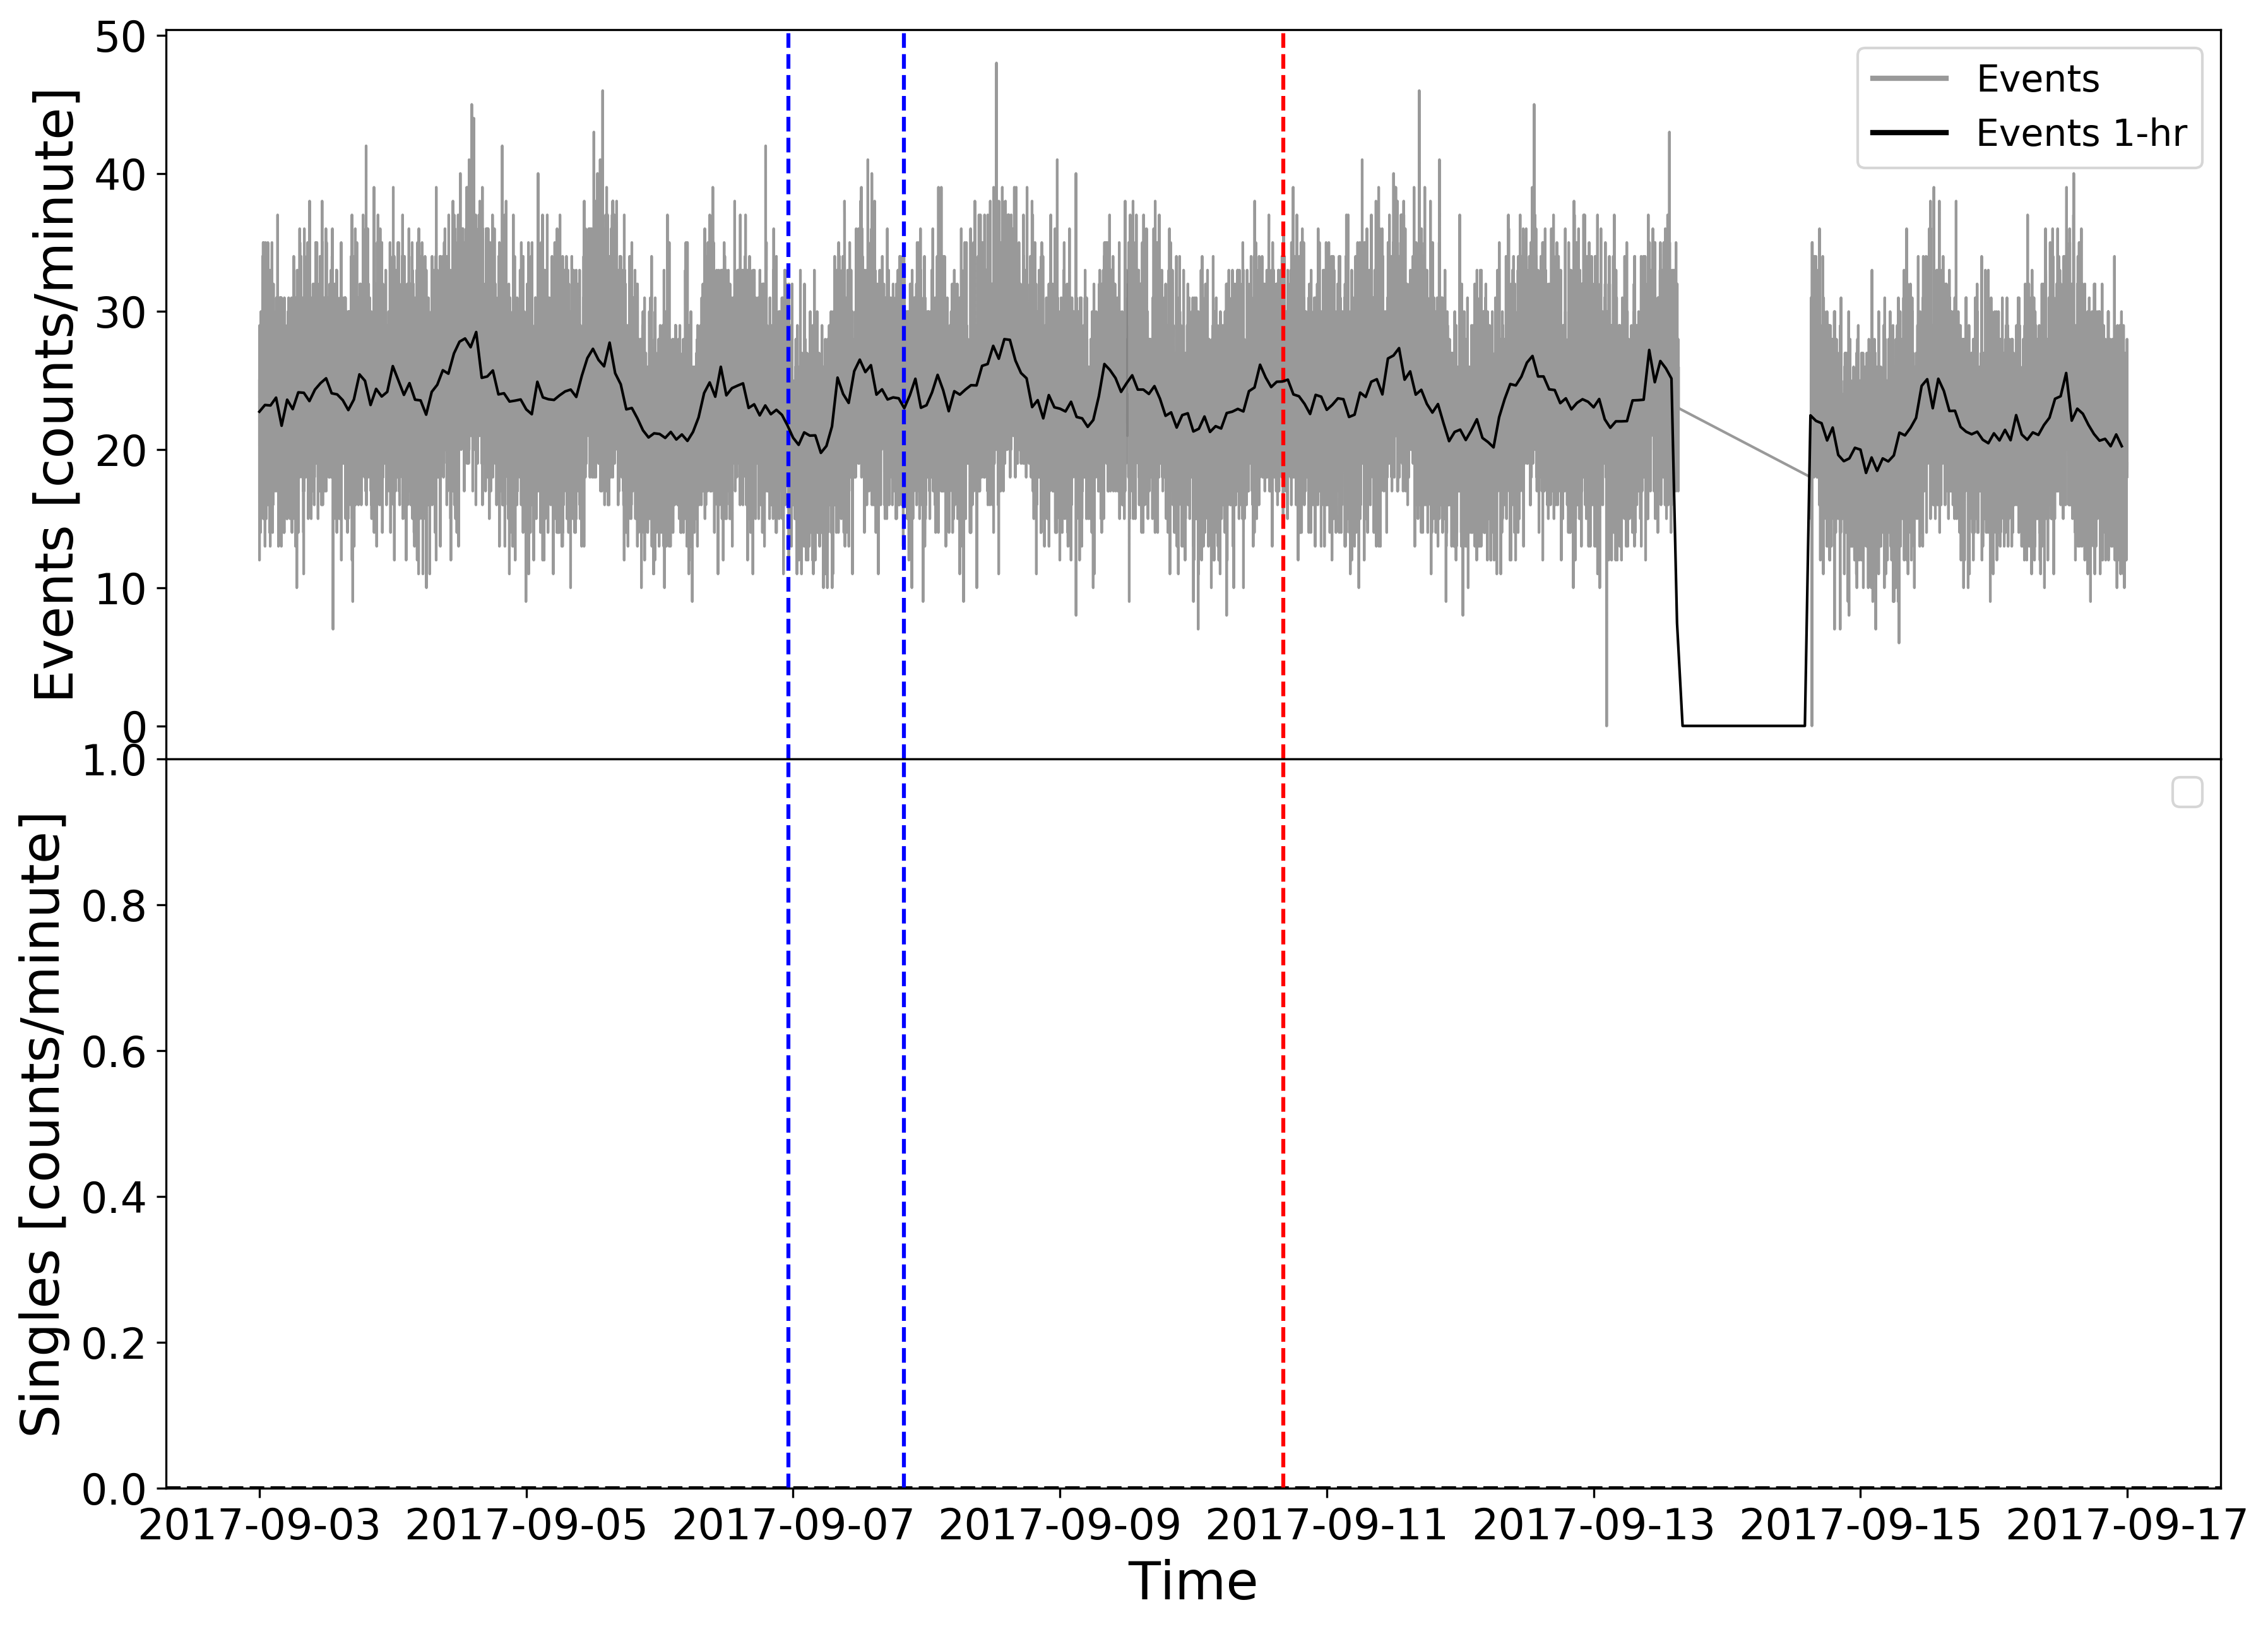
\includegraphics[width=0.48\columnwidth]{FD_GLE72_14001.png}
		\label{fig:FD_GLE72_14001}}
	
	\caption{HiSPARC data for [n] stations around the epoch in which there were several FDs close to the onset of GLE 72. The top panel of each subplot shows the minute-averaged trigger events between detectors within the station, while the bottom panel shows the mean-shifted, minute-averaged counts by each individual detector in the station. The vertical blue-dashed lines show the approximate onset-times of the two FDs observed around this epoch and the red-dashed line depicts the approximate onset time of the GLE.}
	\label{fig:FD_GLE72}
\end{figure}

... no clear FDs seen...



%%%%%%%%%%%%%%%%%%%%%%%%%%%%%%%%%%%%%%%%%%%%%%%%%%%%%%%%%%%%%%%%%%%%%
%%%%%%%%%%%%%%%%%%%%%%%%%%%%%%%%%%%%%%%%%%%%%%%%%%%%%%%%%%%%%%%%%%%%%
\section{Air Shower Simulations}\label{sec:CORSIKA}

In order to understand the footprint of air showers produced by PCRs, simulations of air showers were performed for a range of primary proton and $\alpha$-particle energies.

To simulate the CR air shower development, we employ CORSIKA ({\bf CO}smic {\bf R}ay {\bf SI}mulations for {\bf KA}scade), a Monte Carlo programme providing detailed simulations of the evolution of air showers initiated by cosmic rays particles through the atmosphere \citep{heck_extensive_2017}. The particles in the CORSIKA simulations are tracked through the atmosphere until they undergo interactions with atmospheric nuclei, decay due to their instability, or reach the ground level defined as the end of the simulation.

Proton and $\alpha$-particle initiated air showers were generated with energies ranging from $10^{9}$ to $10^{20}$~eV, and $4\times10^{9}$ to $10^{20}$~eV, respectively. In total $\sim 230000$ proton-initiated showers were simulated and $\sim 180000$ $\alpha$-particle-initiated air showers were simulated. The list of simulated air shower PCRs is shown in Table~\ref{tab:CORSIKA_sims}. For high energy, inelastic hadronic interactions within CORSIKA the QGSJET-II [REF] model was selected. Interactions of hadrons with energies below 80 GeV are simulated using GHEISHA [REF], which allowed for the simulation of PCRs in the regime of SCRs. In addition to these hadronic interactions, electromagnetic interactions within the CORSIKA simulations were described by the EGS4 [REF] model. Furthermore CORSIKA has a minimum muon energy limit that can be simulated of 10 MeV.

\begin{table}
	\begin{center}
	\caption{PCRs simulated using CORSIKA.}
	\label{tab:CORSIKA_sims}
	\begin{tabular}{l r l r | l r l r}
		\hline
		\multicolumn{4}{c}{\bf Protons}  & \multicolumn{4}{c}{\textbf{ $\bm{\alpha}$-Particles}}         \\
		    &    &    &    &    &    &    &    \\
		{\bf E$\bm{_{\mathrm{PCR}}}$ (eV)} & {\bf N$\bm{_{\mathrm{sims}}}$} & {\bf E$\bm{_{\mathrm{PCR}}}$ (eV)} & {\bf N$\bm{_{\mathrm{sims}}}$} & {\bf E$\bm{_{\mathrm{PCR}}}$ (eV)} & {\bf N$\bm{_{\mathrm{sims}}}$} & {\bf E$\bm{_{\mathrm{PCR}}}$ (eV)} & {\bf N$\bm{_{\mathrm{sims}}}$} \\
		\hline
		1.00E+09    & 10000   & 2.98E+12    & 1000    & 4.00E+09    & 10000   & 1.00E+13    & 1000    \\
		1.27E+09    & 10000   & 3.79E+12    & 1000    & 4.28E+09    & 10000   & 1.78E+13    & 100     \\
		1.62E+09    & 10000   & 4.83E+12    & 1000    & 5.46E+09    & 10000   & 3.16E+13    & 100     \\
		2.07E+09    & 10000   & 6.16E+12    & 1000    & 6.95E+09    & 10000   & 5.62E+13    & 100     \\
		2.64E+09    & 10000   & 7.85E+12    & 1000    & 8.86E+09    & 10000   & 1.00E+14    & 100     \\
		3.36E+09    & 10000   & 1.00E+13    & 1000    & 1.00E+10    & 10000   & 1.78E+14    & 50      \\
		4.28E+09    & 10000   & 1.78E+13    & 100     & 1.13E+10    & 10000   & 3.16E+14    & 50      \\
		5.46E+09    & 10000   & 3.16E+13    & 100     & 1.44E+10    & 10000   & 5.62E+14    & 50      \\
		6.95E+09    & 10000   & 5.62E+13    & 100     & 1.83E+10    & 10000   & 1.00E+15    & 10      \\
		8.86E+09    & 10000   & 1.00E+14    & 100     & 2.34E+10    & 10000   & 1.78E+15    & 10      \\
		1.00E+10    & 10000   & 1.78E+14    & 50      & 2.98E+10    & 10000   & 3.16E+15    & 10      \\
		1.13E+10    & 10000   & 3.16E+14    & 50      & 3.79E+10    & 10000   & 5.62E+15    & 10      \\
		1.44E+10    & 10000   & 5.62E+14    & 50      & 4.83E+10    & 10000   & 1.00E+16    & 10      \\
		1.83E+10    & 10000   & 1.00E+15    & 10      & 6.16E+10    & 10000   & 1.78E+16    & 10      \\
		2.34E+10    & 10000   & 1.78E+15    & 10      & 7.85E+10    & 10000   & 3.16E+16    & 10      \\
		2.98E+10    & 10000   & 3.16E+15    & 10      & 1.00E+11    & 10000   & 5.62E+16    & 10      \\
		3.79E+10    & 10000   & 5.62E+15    & 10      & 1.27E+11    & 1000    & 1.00E+17    & 10      \\
		4.83E+10    & 10000   & 1.00E+16    & 10      & 1.62E+11    & 1000    & 1.78E+17    & 10      \\
		6.16E+10    & 10000   & 1.78E+16    & 10      & 2.07E+11    & 1000    & 3.16E+17    & 10      \\
		7.85E+10    & 10000   & 3.16E+16    & 10      & 2.64E+11    & 1000    & 5.62E+17    & 10      \\
		1.00E+11    & 10000   & 5.62E+16    & 10      & 3.36E+11    & 1000    & 1.00E+18    & 10      \\
		1.27E+11    & 1000    & 1.00E+17    & 10      & 4.28E+11    & 1000    & 1.78E+18    & 10      \\
		1.62E+11    & 1000    & 1.78E+17    & 10      & 5.46E+11    & 1000    & 3.16E+18    & 10      \\
		2.07E+11    & 1000    & 3.16E+17    & 10      & 6.95E+11    & 1000    & 5.62E+18    & 10      \\
		2.64E+11    & 1000    & 5.62E+17    & 10      & 8.86E+11    & 1000    & 1.00E+19    & 10      \\
		3.36E+11    & 1000    & 1.00E+18    & 10      & 1.13E+12    & 1000    & 1.78E+19    & 10      \\
		4.28E+11    & 1000    & 1.78E+18    & 10      & 1.44E+12    & 1000    & 3.16E+19    & 10      \\
		5.46E+11    & 1000    & 3.16E+18    & 10      & 1.83E+12    & 1000    & 5.62E+19    & 10      \\
		6.95E+11    & 1000    & 5.62E+18    & 10      & 2.34E+12    & 1000    & 1.00E+20    & 10      \\
		8.86E+11    & 1000    & 1.00E+19    & 10      & 2.98E+12    & 1000    &             &         \\
		1.13E+12    & 1000    & 1.78E+19    & 10      & 3.79E+12    & 1000    &             &         \\
		1.44E+12    & 1000    & 3.16E+19    & 10      & 4.83E+12    & 1000    &             &         \\
		1.83E+12    & 1000    & 5.62E+19    & 10      & 6.16E+12    & 1000    &             &         \\
		2.34E+12    & 1000    & 1.00E+20    & 10      & 7.85E+12    & 1000    &             &         \\   
		\hline
	\end{tabular}
	\end{center}
\end{table}

There are several other user-definable setting within CORSIKA which are explained in-depth in the CORSIKA user's guide \citep{heck_extensive_2017}. The settings chosen within these simulation are breifly discussed below. Simulation thinning was enable in CORSIKA to reduce computation time and reduce the output file size. The observation level at which point the simulation cease was set at 100 m above sea level (compared to the $\sim 50$ m typical of the stations, however this difference is negligible for the air shower development.) The pre-defined central European atmosphere in October was used for all simulations, and western-European magnetic field was used as calculated with the \textit{Geomag} programme [REF]: B$_{\mathrm{x}}=18.799$~$\mu$T and B$_{\mathrm{z}}=44.980$~$\mu$T.


%%%%%%%%%%%%%%%%%%%%%%%%%%%%%%%%%%%%%%%%%%%%%%%%%%%%%%%%%%%%%%%%%%%%%
\subsection{Air Shower Footprints}\label{sec:CORSIKA_footprint}

The average footprint of muons at ground level was acquired from the output CORSIKA simulations. This was achieved by simply taking the distributino of the muons at ground level at the end of the simulation as a function of their distance from the shower core for each individual simulation realisation. For a given PCR energy the average air shower footprint distribution is calculated by combining the individual simulation realisations.

%[Discuss how distance between the HiSPARC station 2d/4d detectors will impact the ability to view certain PCR energies, and sets an lower limit on the energies observable in the standard trigger mode]

\begin{figure}
	\centering
	\subfloat[Proton initiated air shower. \label{fig:p_footprint}]{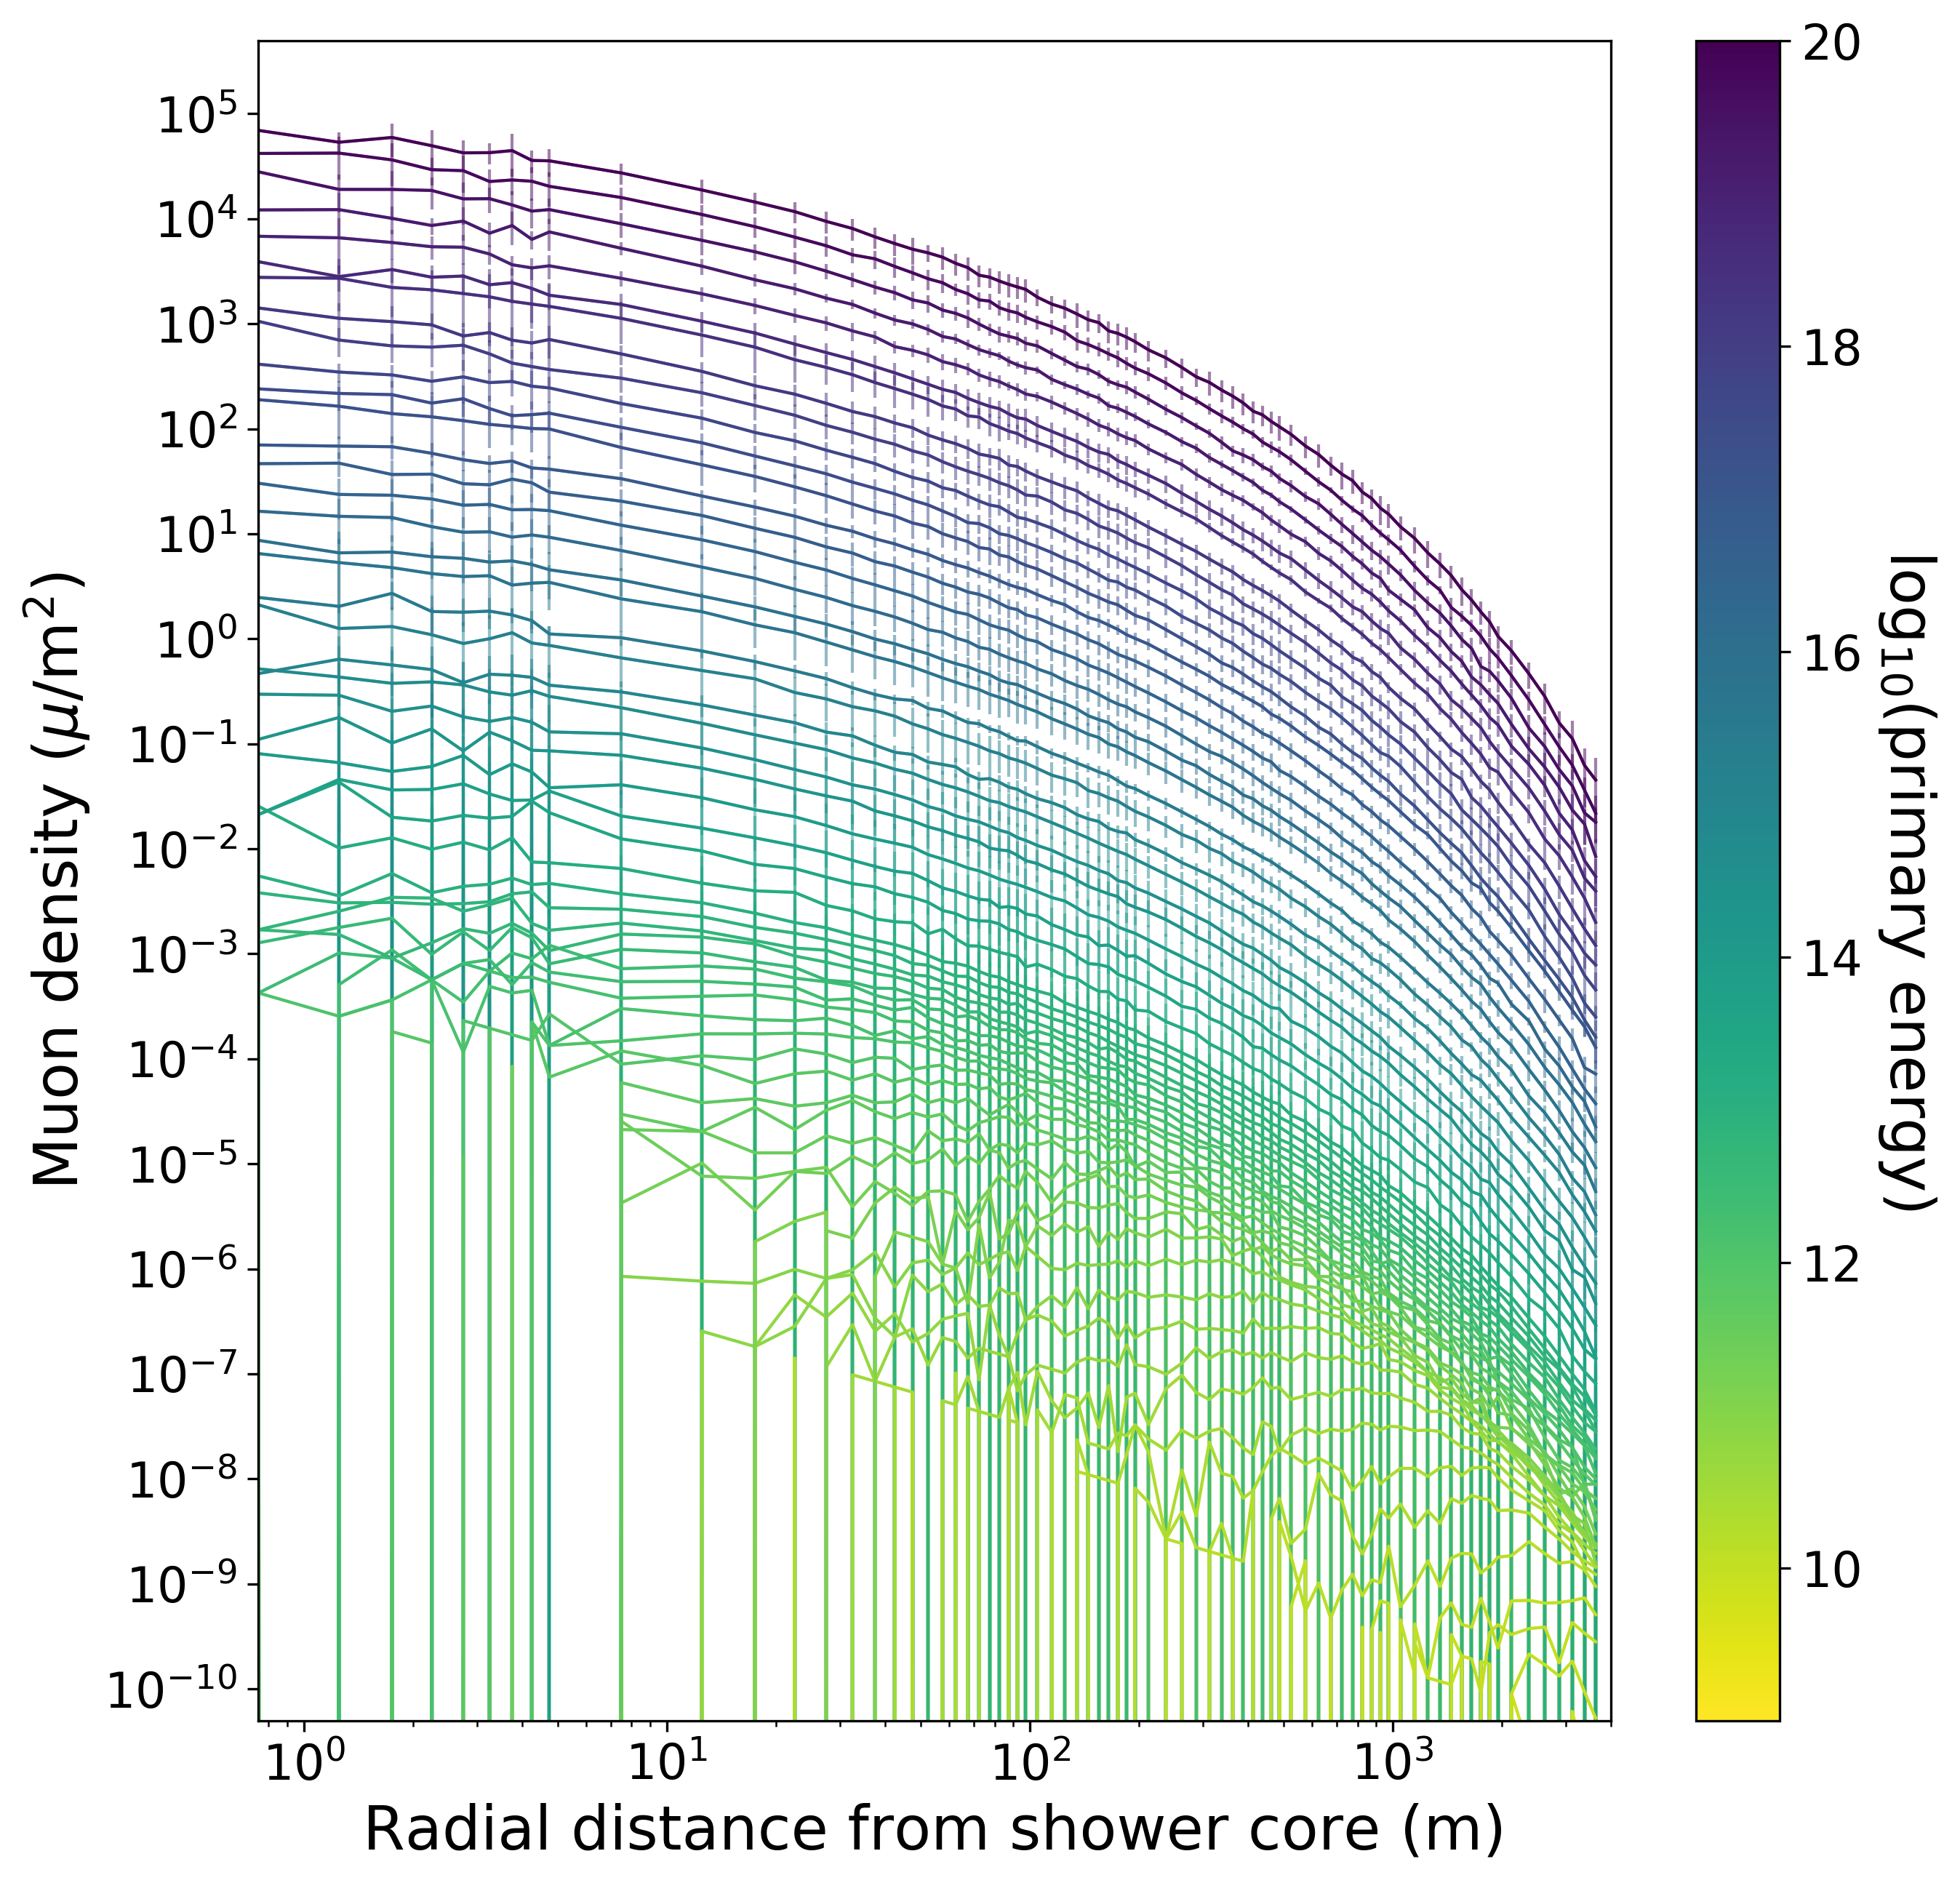
\includegraphics[width=0.47\columnwidth]{proton_footprint.png}} 
	\qquad
	\subfloat[$\alpha$-particle initiated air shower. \label{fig:a_footprint}]{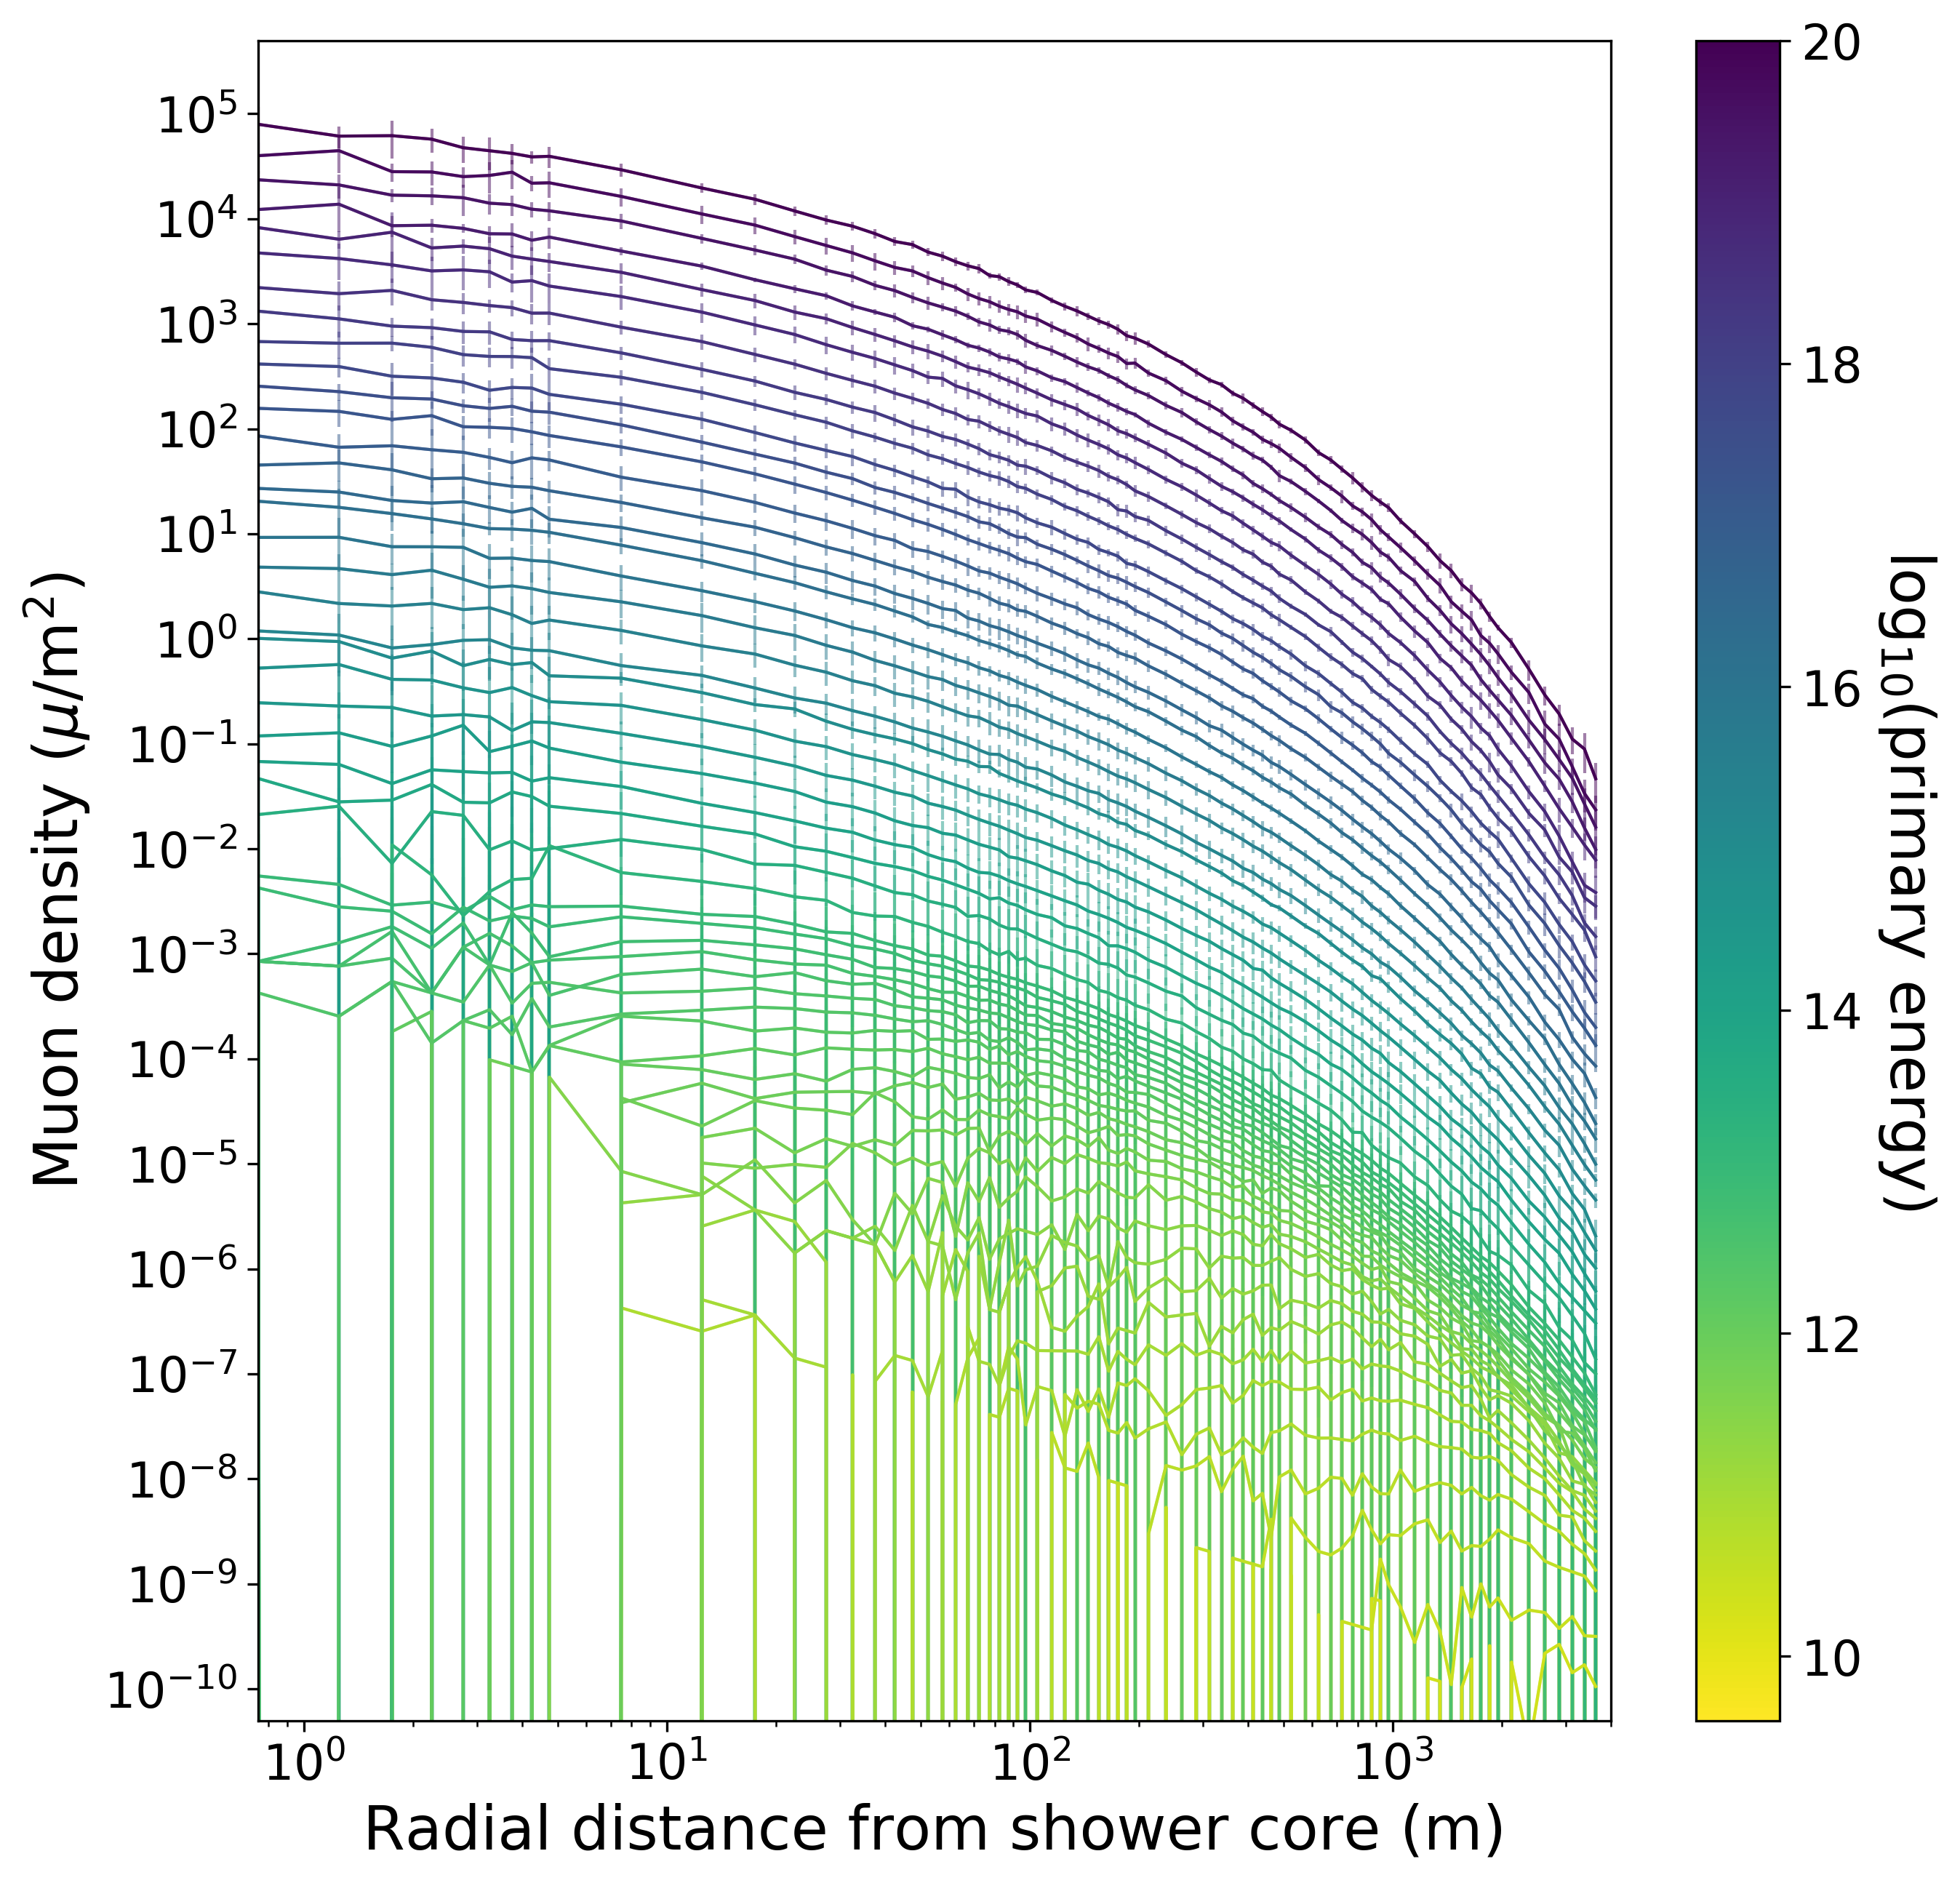
\includegraphics[width=0.47\columnwidth]{alpha_footprint.png}}
	\caption{Mean muon density footprints for (a) proton-initiated air showers and (b) $\alpha$-particle-initiated air showers with intial PCR trajectories with zenith angles $\theta=0^{\circ}$ and various PCR energies. The error bars given represent 1$\sigma$.} \label{fig:shower_footprints}
\end{figure}

The interpretation of Figure~\ref{fig:shower_footprints} can provide an understanding of the minimum energy of PCRs observable by the different stations within the HiSPARC network. The typical separation between the detectors in a HiSPARC station is $\sim 10$~m, however the separation between detectors can be up to as much as 20~m or as low as a couple of metres. This analysis of the air shower footprint shows the variation in PCR energy sampled varies marginally over this range of distances and suggests that HiSPARC stations will typical observe PCR with an energy of $\sim 10^{14}-10^{15}$~eV to meet the required trigger conditions.

%\begin{table}
%	\begin{center}
%		\caption{HS station minimum observable PCR energy}
%		\label{tab:footprints}
%		\begin{tabular}{l c c c}
%		\hline
%		{Station ID} & {Average separation (m)} & {Proton E$_{\mathrm{min}}$} & {$\alpha$-particle E$_{\mathrm{min}}$} \\
%		\hline
%		{501} & {11.2} & {} & {} \\
%		{14001} & {9.1} & {} & {} \\
%		{} & {} & {} & {} \\
%		\hline
%\end{tabular}
%\end{center}
%\end{table}


\subsection{Muon Flux}\label{sec:CORSIKA_flux}

From the air shower simulations it is possible to gain an estimate of the muon flux at groud-level based on the number of 

\begin{figure}
	\centering
	\subfloat[Proton initiated air shower. \label{fig:p_muons}]{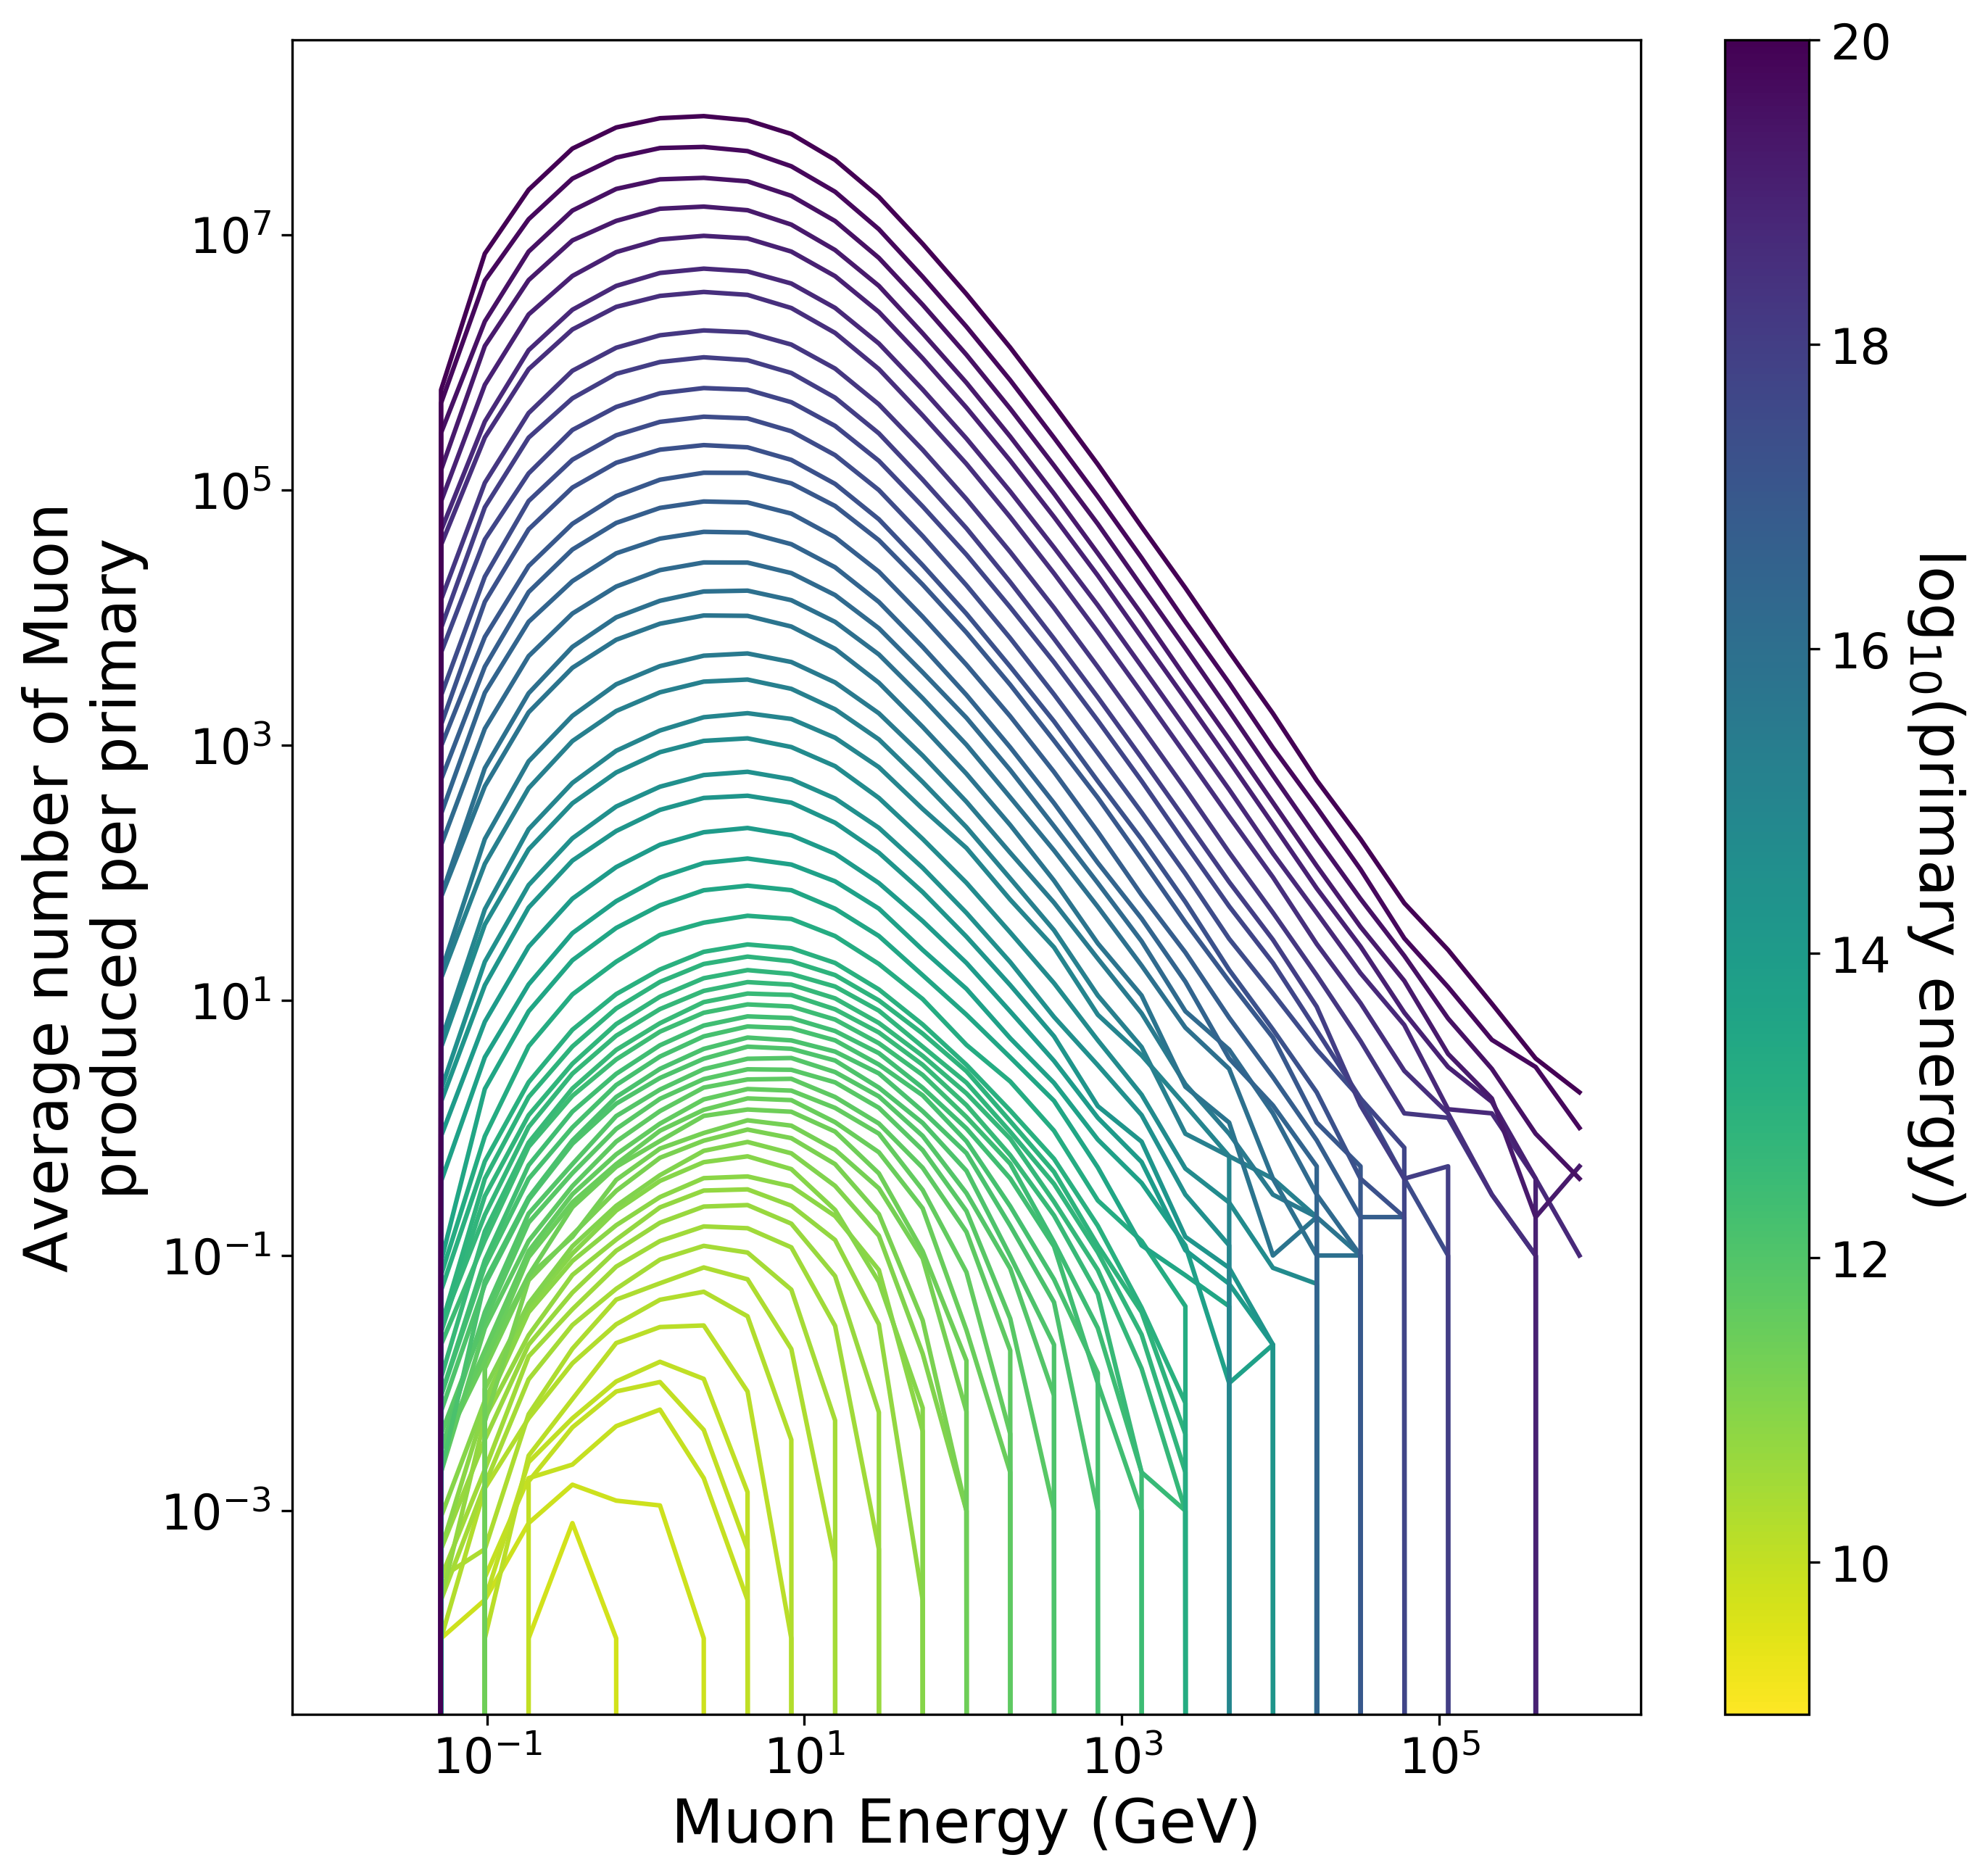
\includegraphics[width=0.47\columnwidth]{proton_muon_number.png}} 
	\qquad
	\subfloat[$\alpha$-particle initiated air shower. \label{fig:a_muons}]{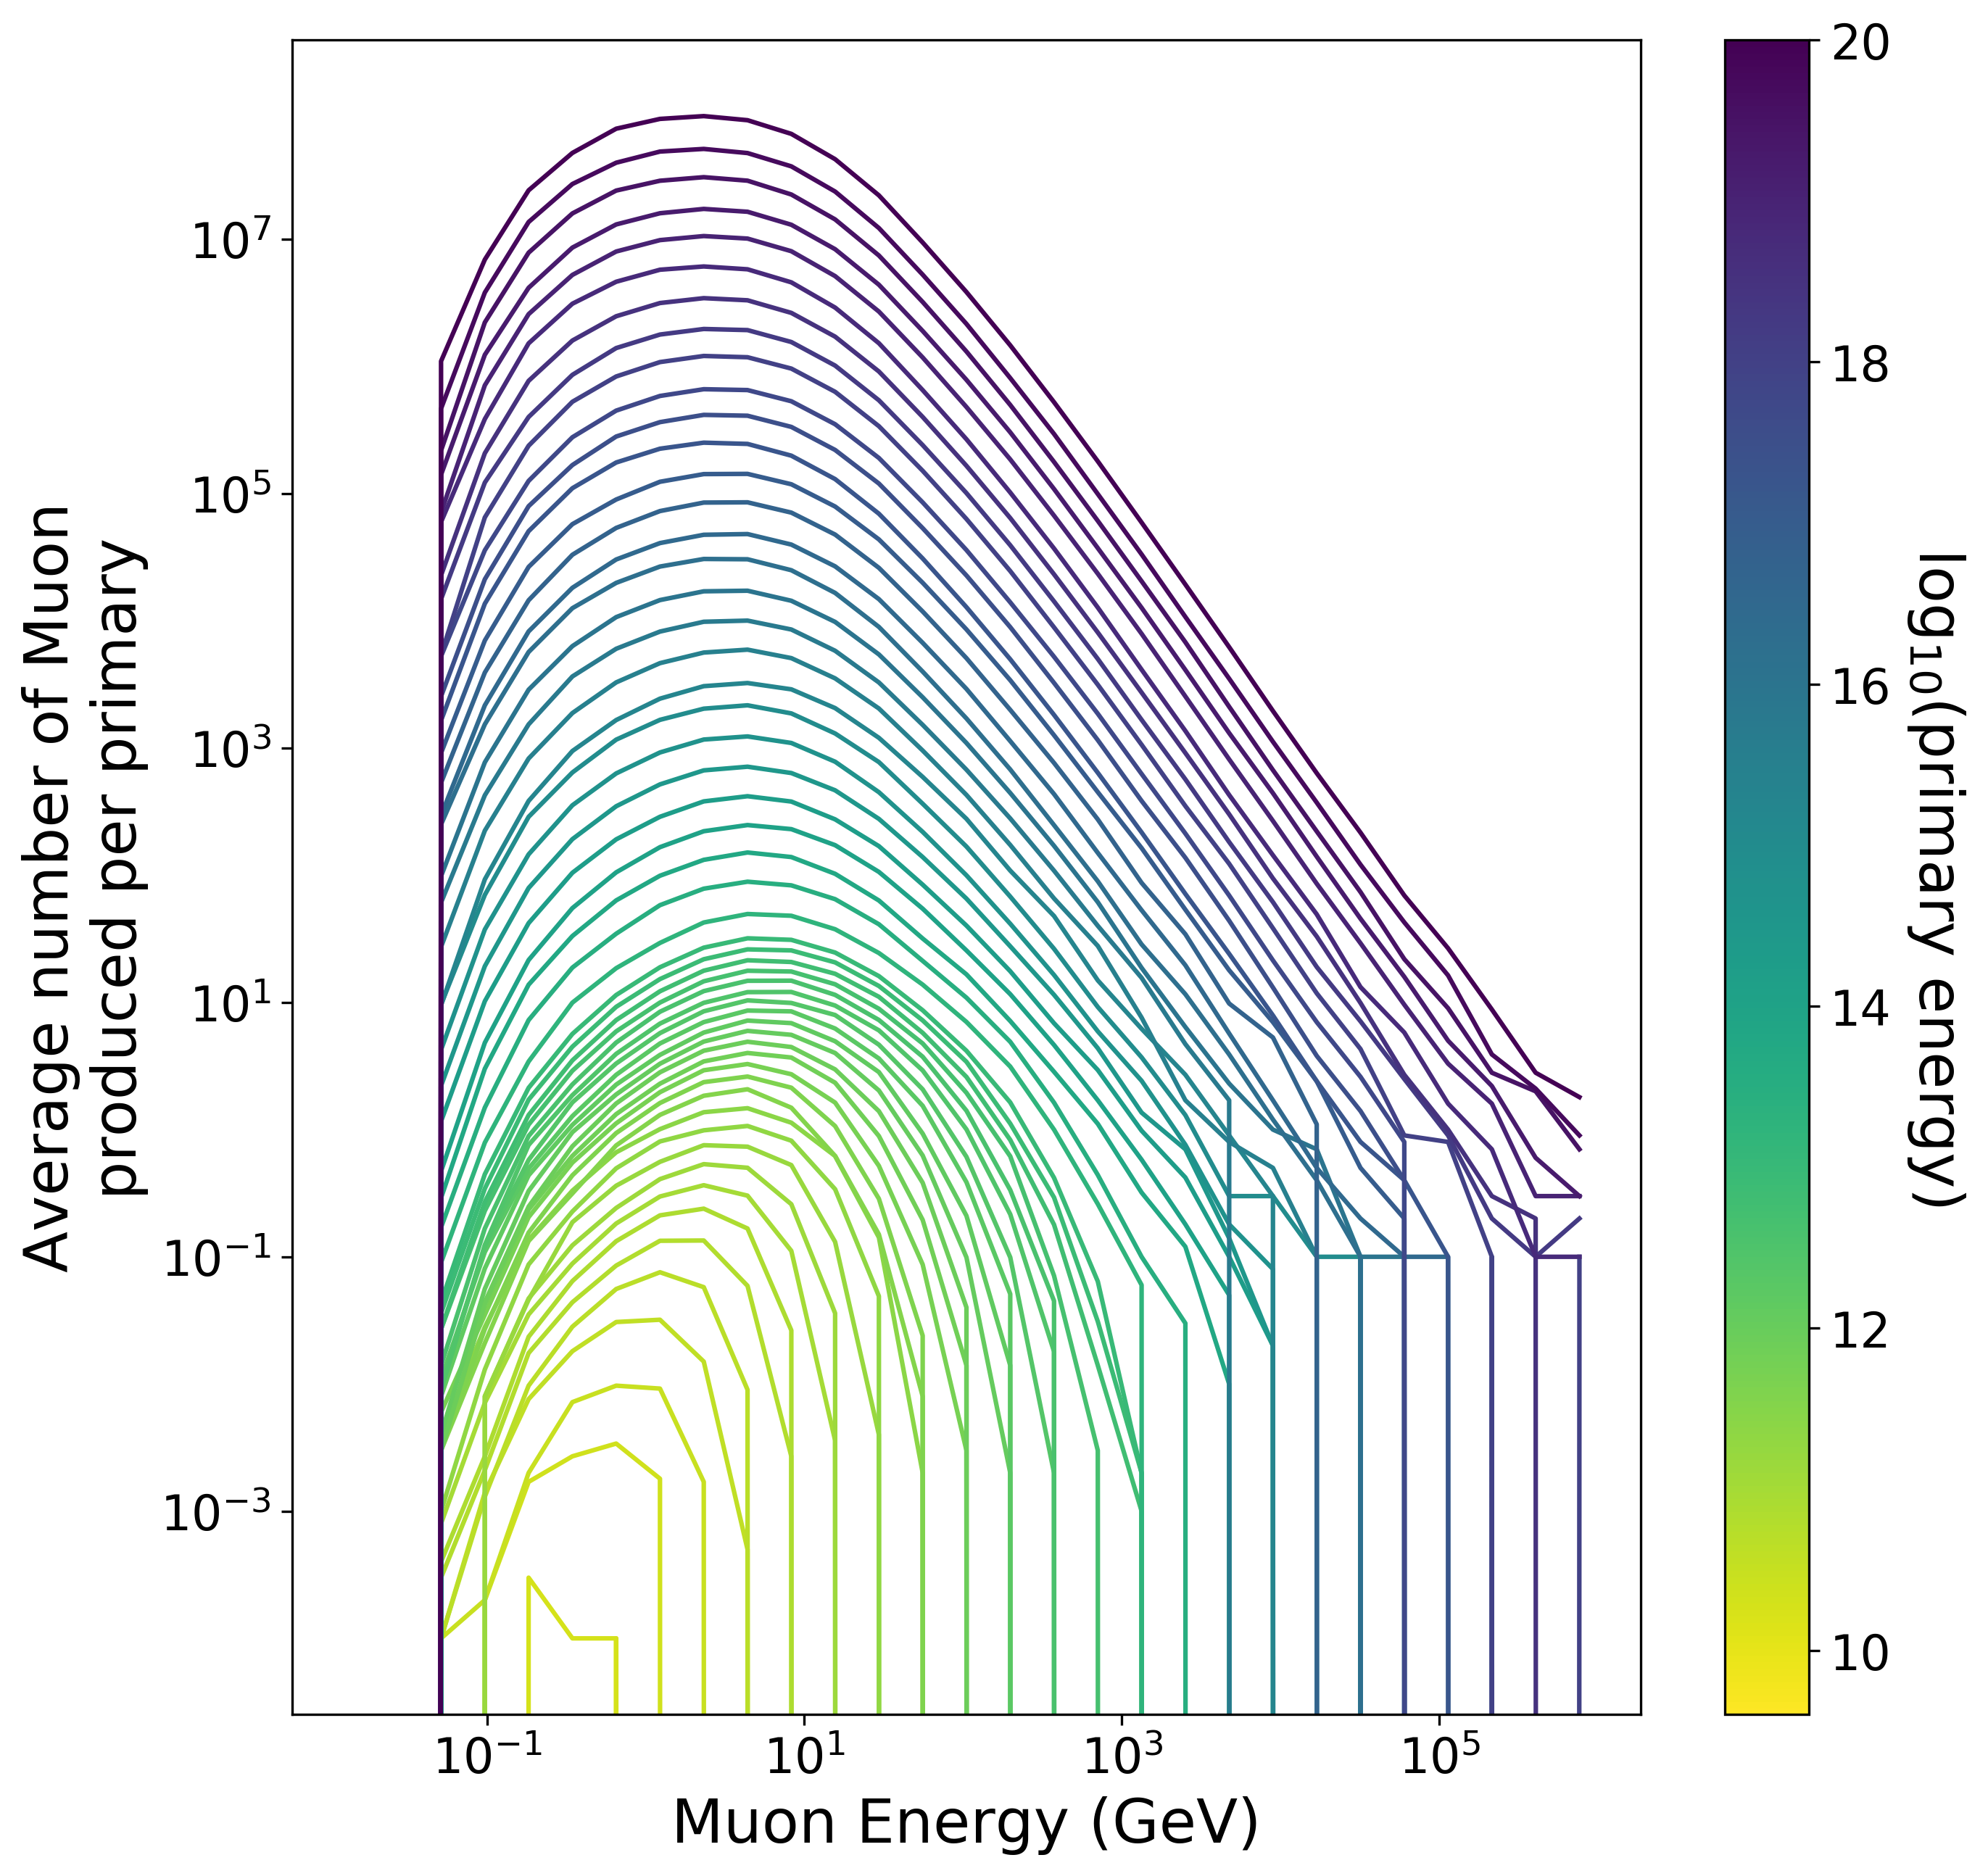
\includegraphics[width=0.47\columnwidth]{alpha_muon_number.png}}
	\caption{Mean number of muons produced at ground level by the PCR for (a) proton-initiated air showers and (b) $\alpha$-particle-initiated air showers, for various PCR energy. The uncertainty bars given represent 1$\sigma$.}
	\label{fig:shower_muons}
\end{figure}



%%%%%%%%%%%%%%%%%%%%%%%%%%%%%%%%%%%%%%%%%%%%%%%%%%%%%%%%%%%%%%%%%%%%%
%%%%%%%%%%%%%%%%%%%%%%%%%%%%%%%%%%%%%%%%%%%%%%%%%%%%%%%%%%%%%%%%%%%%%
\section{Standardisation of HiSPARC Data}\label{sec:HS_standardisation}

%%%%%%%%%%%%%%%%%%%%%%%%%%%%%%%%%%%%%%%%%%%%%%%%%%%%%%%%%%%%%%%%%%%%%
\subsection{Motivation}

%%%%%%%%%%%%%%%%%%%%%%%%%%%%%%%%%%%%%%%%%%%%%%%%%%%%%%%%%%%%%%%%%%%%%
\subsection{Barometric Correction}\label{sec:HS_P_corr}

It is understood that observations made by ground-based CR detectors are susceptible to atmospheric conditions. Atmospheric pressure effects the CR travel path due to the expansion and contraction of the atmosphere with varying pressure; hence the CR counts are observed to be negatively correlated to atmospheric pressure [add example plot to show].

The method of correcting for the barometric effect is discussed widely in the neutron monitor literature and is shown to depend on the barometric coefficient. If the cosmic ray flux is constant, $N$, CR variations depend on the local atmospheric pressure as described by equation~(\ref{eq:presscorr1}), where $\Delta N$ is the change in count rate, $\beta$ is the barometric coefficient, and $\Delta P = P - P_0$ is the deviation in pressure from the average ($P_0$) in the given time-period \citep{paschalis_online_2013}:

\begin{equation}
\Delta N = - \beta \, N \, \Delta P
\label{eq:presscorr1}
\end{equation}

Through the integration of equation~(\ref{eq:presscorr1}), the solution shows the dependence of cosmic ray intensity on pressure as in equation~(\ref{eq:presscorr2}). 

\begin{equation}
N = N_{0} \, e^{-\beta \, \Delta P}
\label{eq:presscorr2}
\end{equation}

Therefore by taking the natural logarithm of equation~(\ref{eq:presscorr2}), one can obtain the barometric coefficient through fitting the straight line in equation~(\ref{eq:presscorr3}) to the observed data, where $N_0$ may be assumed as the average count rate over the given time-period. 

\begin{equation}
\mathrm{ln} \left( \frac{\Delta N}{N} \right) = - \beta \, \Delta P
\label{eq:presscorr3}
\end{equation}


%%%%%%%%%%%%%%%%%%%%%%%%%%%%%%%%%%%%%%%%%%%%%%%%%%%%%%%%%%%%%%%%%%%%%
\subsection{Temperature Correction}\label{sec:HS_T_corr}




